
%%%%%%%%%%%%%%%%%%%%%%%%%%%%%%%%%%%%%%%%%
% Beamer Presentation
% LaTeX Template
% Version 1.0 (10/11/12)
%
% This template has been downloaded from:
% http://www.LaTeXTemplates.com
%
% License:
% CC BY-NC-SA 3.0 (http://creativecommons.org/licenses/by-nc-sa/3.0/)
%
%%%%%%%%%%%%%%%%%%%%%%%%%%%%%%%%%%%%%%%%%

%----------------------------------------------------------------------------------------
%	PACKAGES AND THEMES
%----------------------------------------------------------------------------------------

\documentclass{beamer}

\mode<presentation> {

% The Beamer class comes with a number of default slide themes
% which change the colors and layouts of slides. Below this is a list
% of all the themes, uncomment each in turn to see what they look like.

%\usetheme{default}
%\usetheme{AnnArbor}
%\usetheme{Antibes}
%\usetheme{Bergen}
%\usetheme{Berkeley}
%\usetheme{Berlin}
%\usetheme{Boadilla}
%\usetheme{CambridgeUS}
%\usetheme{Copenhagen}
%\usetheme{Darmstadt}
%\usetheme{Dresden}
%\usetheme{Frankfurt}
%\usetheme{Goettingen}
%\usetheme{Hannover}
%\usetheme{Ilmenau}
%\usetheme{JuanLesPins}
%\usetheme{Luebeck}
\usetheme{Madrid}
%\usetheme{Malmoe}
%\usetheme{Marburg}
%\usetheme{Montpellier}
%\usetheme{PaloAlto}
%\usetheme{Pittsburgh}
%\usetheme{Rochester}
%\usetheme{Singapore}
%\usetheme{Szeged}
%\usetheme{Warsaw}

% As well as themes, the Beamer class has a number of color themes
% for any slide theme. Uncomment each of these in turn to see how it
% changes the colors of your current slide theme.

%\usecolortheme{albatross}
%\usecolortheme{beaver}
%\usecolortheme{beetle}
%\usecolortheme{crane}
\usecolortheme{dolphin}
%\usecolortheme{dove}
%\usecolortheme{fly}
%\usecolortheme{lily}
%\usecolortheme{orchid}
%\usecolortheme{rose}
%\usecolortheme{seagull}
%\usecolortheme{seahorse}
%\usecolortheme{whale}
%\usecolortheme{wolverine}

%\setbeamertemplate{footline} % To remove the footer line in all slides uncomment this line
%\setbeamertemplate{footline}[page number] % To replace the footer line in all slides with a simple slide count uncomment this line

%\setbeamertemplate{navigation symbols}{} % To remove the navigation symbols from the bottom of all slides uncomment this line
}

\usepackage{graphicx} % Allows including images
\usepackage{booktabs} % Allows the use of \toprule, \midrule and \bottomrule in tables
\usepackage{array}
\usepackage{tabularx}
\usepackage[backend=biber,style=apa]{biblatex}
\addbibresource{references.bib}
\usepackage{hyperref}
\usepackage{changepage}
\usepackage[hang,flushmargin]{footmisc}
\usepackage[normalem]{ulem}
\hypersetup{
	colorlinks,
    citecolor={blue!70!black},
	linkcolor={blue!70!black},
	urlcolor={blue!70!black}}

\usepackage{appendixnumberbeamer}
\usepackage{amsmath}
\usepackage{booktabs}      % For \toprule, \midrule, \bottomrule
\usepackage{threeparttable} % For tablenotes
\usepackage{tikz}
\usetikzlibrary{arrows.meta}

%\setbeamercolor{alerted text}{fg=red!70!black}    % warm alert
%\setbeamercolor{alerted text}{fg=orange!80!black} % another option
%\setbeamercolor{alerted text}{fg=cyan!60!black} 

\definecolor{AlertOrangeRed}{RGB}{255,69,0}
\definecolor{AlertDarkOrange}{RGB}{255,140,0}
\definecolor{AlertTomato}{RGB}{255,99,71}
\definecolor{AlertCoral}{RGB}{255,127,80}
\definecolor{AlertGold}{RGB}{255,215,0}
\definecolor{AlertYellowOrange}{RGB}{255,174,66}
\definecolor{AlertMagenta}{RGB}{255,0,255}
\definecolor{AlertVermilion}{RGB}{227,66,52}

% Set default alert color (global)
\setbeamercolor{alerted text}{fg=AlertOrangeRed}
\setbeamertemplate{navigation symbols}{}     % remove all navigation symbols
%\setbeamertemplate{footline}{}  \beamertemplatenavigationsymbolsempty

%----------------------------------------------------------------------------------------
%	TITLE PAGE
%----------------------------------------------------------------------------------------

\title[Tax Evasion and Tax Filing Costs]{Tax Evasion and Tax Filing Costs: \\
Considerations and Support for Third-Party Reporting} % The short title appears at the bottom of every slide, the full title is only on the title page

\author[Kircali, Stantcheva and Weber] % Short author list for footer
{Tim Kircali\inst{1} \and Stefanie Stantcheva\inst{2} \and Matthias Weber\inst{1}}

\institute[] % Short institution list for footer
{
\inst{1} University of St.Gallen \\
\inst{2} Harvard University
}
{
\medskip

}

\date[February 2026]{Talk w. Stefanie, February 2026}
 % Date, can be changed to a custom date

\begin{document}

\begin{frame}
\titlepage % Print the title page as the first slide
\end{frame}

\begin{frame}
\frametitle{Overview for Today}
\begin{itemize}
    \item Topics that we should discuss today\vspace{0.5em}
    \begin{enumerate}
        \item Information treatments \vspace{0.5em}
        \item Update on data to enforce/prepopulate \vspace{0.5em}
        \item Survey questions and estimation/pre-analysis plan\vspace{1.5em}
    \end{enumerate}
    \item Next steps \vspace{0.5em}
    \begin{enumerate}
        \item Incorporation of remaining feedback \vspace{0.5em}
        \item Run pilot \vspace{1.5em}
    \end{enumerate}
    \item Additional points \vspace{0.5em}
    \begin{enumerate}
        \item Think about a new title? \vspace{0.5em}
        \item Schedule monthly meetings? \vspace{0.5em}
    \end{enumerate}
\end{itemize}
\end{frame}

\begin{frame}
\frametitle{1) Information Treatments}
\label{frame:treatments}
  \centering
  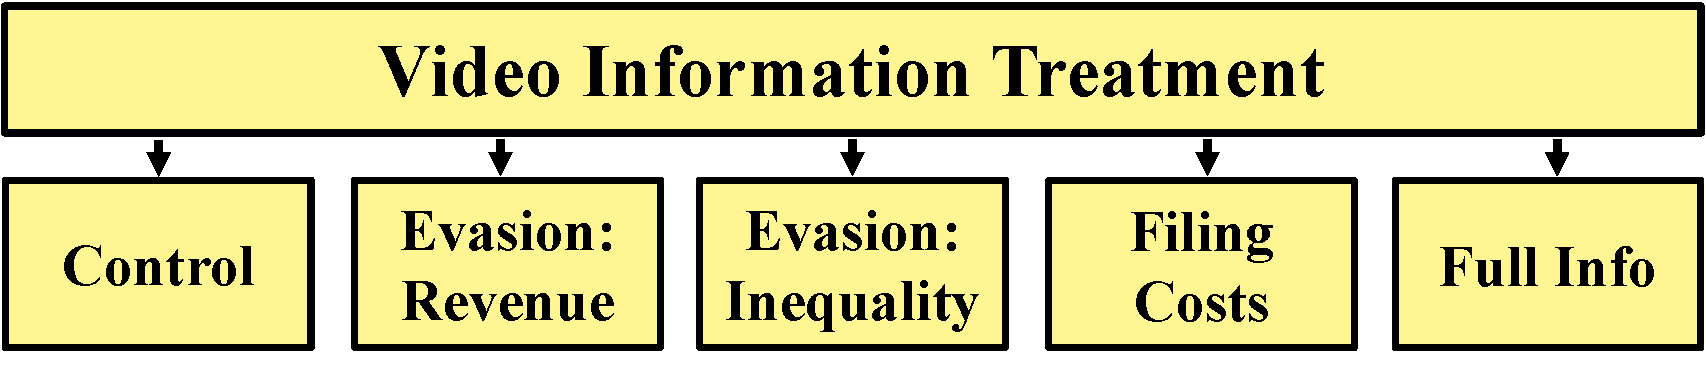
\includegraphics[width=0.7\textwidth]{Figures_Slides/Survey_Overview_Treatments_Focus.pdf}

  \vspace{0.5cm}
\centering
{\scriptsize
\begin{tabularx}{\textwidth}{*{4}{>{\centering\arraybackslash}X}}
  \textbf{Evasion: Revenue} & \textbf{Evasion: Inequality} & \textbf{Filing Costs} & \textbf{Full information} \\[0.5em]
  \textbf{1:48 min}  &
  \textbf{2:26 min}  &
  \textbf{2:56 min}  &
  \textbf{5:07 min} \\[0em]
  \begin{itemize}\item[$\Rightarrow$] Tax Evasion \& Government Revenue\end{itemize} &
  \begin{itemize}\item[$\Rightarrow$] Tax Evasion \& Government Revenue\end{itemize} &
   &
  \begin{itemize}\item[$\Rightarrow$] Tax Evasion \& Government Revenue\end{itemize} \\[-1em]
  &
  \begin{itemize}\item[$\Rightarrow$] Fairness \& Inequality\end{itemize} &
  &
  \begin{itemize}\item[$\Rightarrow$] Fairness \& Inequality\end{itemize} 
  \\[-1em]
&
&
  \begin{itemize}\item[$\Rightarrow$] Filing Costs \end{itemize} &
  \begin{itemize}\item[$\Rightarrow$] Filing Costs \end{itemize} \\
  \centering \hyperlink{frame:Evasionrevenue}{\beamergotobutton{Evasion: Revenue}}&
  \centering \hyperlink{frame:Evasioninequality}{\beamergotobutton{Evasion: Inequality}}&
  \centering \hyperlink{frame:Taxfiling}{\beamergotobutton{Filing Costs}}& 
  \centering \hyperlink{frame:Fullinfo}{\beamergotobutton{Full Info}}
\end{tabularx}
} \\

\end{frame}

\begin{frame}
\frametitle{2) Updates: Data to Prepopulate/Enforce}

\begin{columns}[T,onlytextwidth]

% Left box
\begin{column}{0.48\textwidth}
\textbf{Data to enforce taxes} \\[0.5em]
IRS lacks detailed data on:
\begin{enumerate}
    \item Sole proprietorships
    \item Pass-through businesses\footnotemark[1]
    \item Other income sources\footnotemark[2]
    \vspace{1em}
    \item[$\rightarrow$] Difficult to address due to administrative burden for reporting parties.
    \item[$\rightarrow$] Focus on platforms, banks, and businesses to report aggregate amounts.
\end{enumerate}
\end{column}
\begin{column}{0.04\textwidth}
\end{column}
% Right box
\begin{column}{0.48\textwidth}
\textbf{Data to prepopulate} \\[0.5em]
First, IRS lacks detailed data on:
\begin{enumerate}
    \item State and local taxes, credits and benefits
    \item Charitable contributions
    \item Other deductible expenses\footnotemark[3]
\end{enumerate}
\vspace{0.5em}
Second, data is not processed before the filing deadline due to: 
\begin{enumerate}
    \item Extension available to report.
    \item Capacity issues in IRS processing.
\end{enumerate}

\end{column}

\end{columns}

\footnotetext[1]{E.g. partnerships and S corporations}
\footnotetext[2]{E.g. rents and royalties, income from estates and trusts, gains from the sale of business property, farming income, alimony, and gambling winnings.}
\footnotetext[3]{E.g. medical expenses}

\end{frame}

\begin{frame}
\frametitle{2) Updates: New Version of TPR Policy}
\label{Update2}
\textbf{Old version}: "$\dots$ In a comprehensive third-party reporting system, the tax authority receives detailed and automatic reports from many sources."
\begin{itemize}
    \item[$\rightarrow$] \alert{Critique received as the policy is held too general.}
\end{itemize}
\vspace{1em}

\textbf{New version}: The policy consists of three components:
\begin{enumerate}
    \item Introducing aggregate bank flow reporting.\footnote[4]{The Biden administration proposed in 2021 to introduce aggregate bank flow reporting, whereby banks would be required to report inflows and outflows for all accounts above a certain (low) threshold.} 
    \item Transmitting previously unreported information on taxes paid at the local level to the IRS.
    \item Ensuring that reported data are received more quickly.
    \vspace{0.5em}
    \item[$\rightarrow$] \alert{Precise and understandable policy.}
    \item[$\rightarrow$] \alert{Potential to reduce tax evasion and tax filing costs.}
    \item[$\rightarrow$] \alert{Aligns with the policy debate in the U.S.} \hfill \hyperlink{DetailedPolicies}{\beamergotobutton{Policies}}
\end{enumerate}

\end{frame}

\begin{frame}
\label{pretreatment}
\frametitle{3) Survey \& Estimation: Pre Treatment}
\begin{columns}[T] % align columns at the top
  \begin{column}{0.45\textwidth} % left side for text
  \begin{enumerate}
    \item Prolific quota sample\\
    \hyperlink{Quotas}{\beamergotobutton{Sample and Quality}} 
    \item Demographic background
    \begin{itemize}
        \item[$\rightarrow$] aligns with census data, which we can then use to test representativeness. 
    \end{itemize} %\vspace{0.25em}
    \item Government views and (general) views on inequality %\vspace{0.25em}
    \item Policy exposure 
    \begin{itemize}
        \item to tax filing
        \item to tax software
        \item to filing mistakes
        \item to tax evasion
    \end{itemize} %\vspace{0.25em}
    \item[$\Rightarrow$] \alert{Pre treatment variables will be used as control variables.}  \hyperlink{Controlvariables}{\beamergotobutton{Control Variables}}
  \end{enumerate}
  \end{column}
  
  \begin{column}{0.45\textwidth} % right side for image
    \centering
     \vspace{-1em}     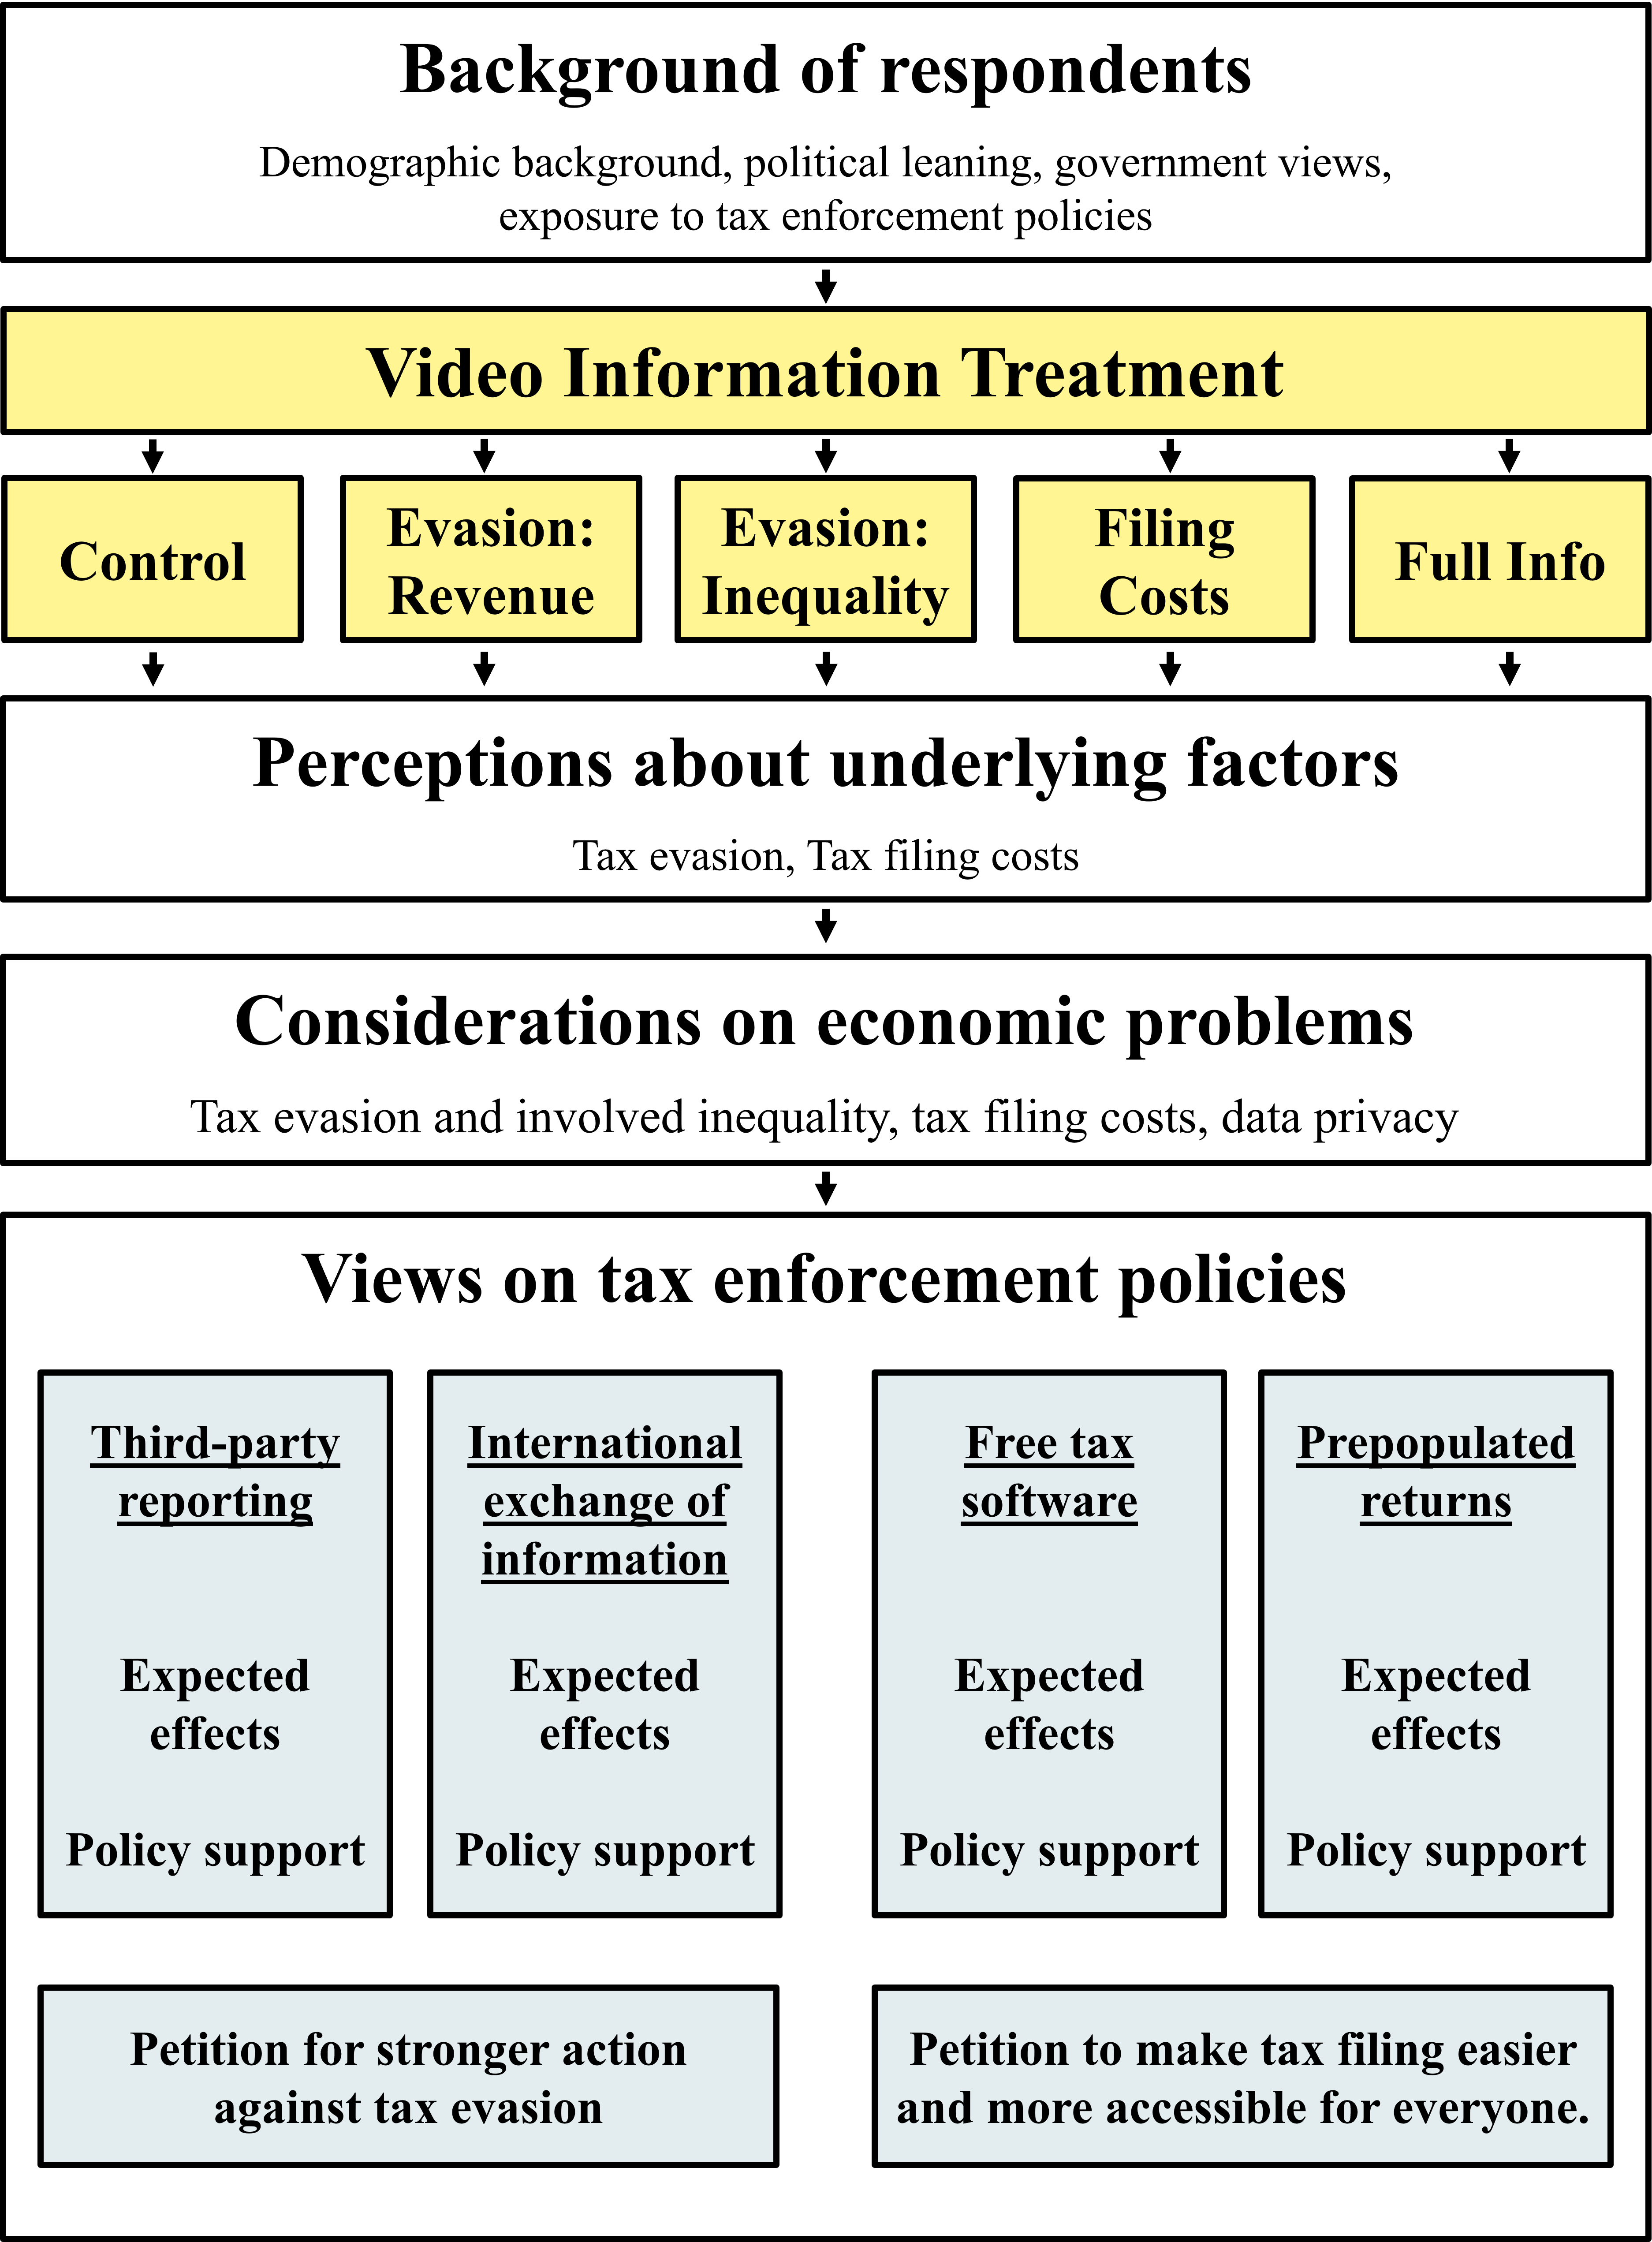
\includegraphics[width=1.05\linewidth]{Figures_Slides/Survey_Overview_Treatments.png}
  \end{column}
\end{columns}
    
\end{frame}


\begin{frame}{3) Survey \& Estimation: Post Treatment}
\label{posttreatment}
\begin{columns}[T] % align columns at the top
  \begin{column}{0.45\textwidth} % left side for text
  \begin{itemize}
      \item Perception / Knowledge
      \hyperlink{Example:Knowledge}{\beamergotobutton{}}\vspace{0.5em}
      \item Considerations on underlying economic problems \hyperlink{Example:ConsiderationsEconomicProblems}{\beamergotobutton{}} \vspace{0.5em}
      \item Views on policies \vspace{0.25em} 
      \begin{itemize}
          \item Expected effects: \hyperlink{Example:ExpectedEffects}{\beamergotobutton{}}\vspace{0.25em} 
        \begin{itemize}
            \item revenue
            \item inequality 
            \item filing costs 
            \item data privacy
        \end{itemize}
        \vspace{0.25em} 
          \item Policy support: 
          \begin{itemize}
              \item general \hyperlink{Example:PolicySupportGen}{\beamergotobutton{}}
              \item conditional \hyperlink{Example:PolicySupportCond}{\beamergotobutton{}}
          \end{itemize} 
           \vspace{0.25em} 
          \item Petition: validate support
      \end{itemize}
  \end{itemize}
  \end{column}
  
  \begin{column}{0.45\textwidth} % right side for image
    \centering
     \vspace{-0.5em}     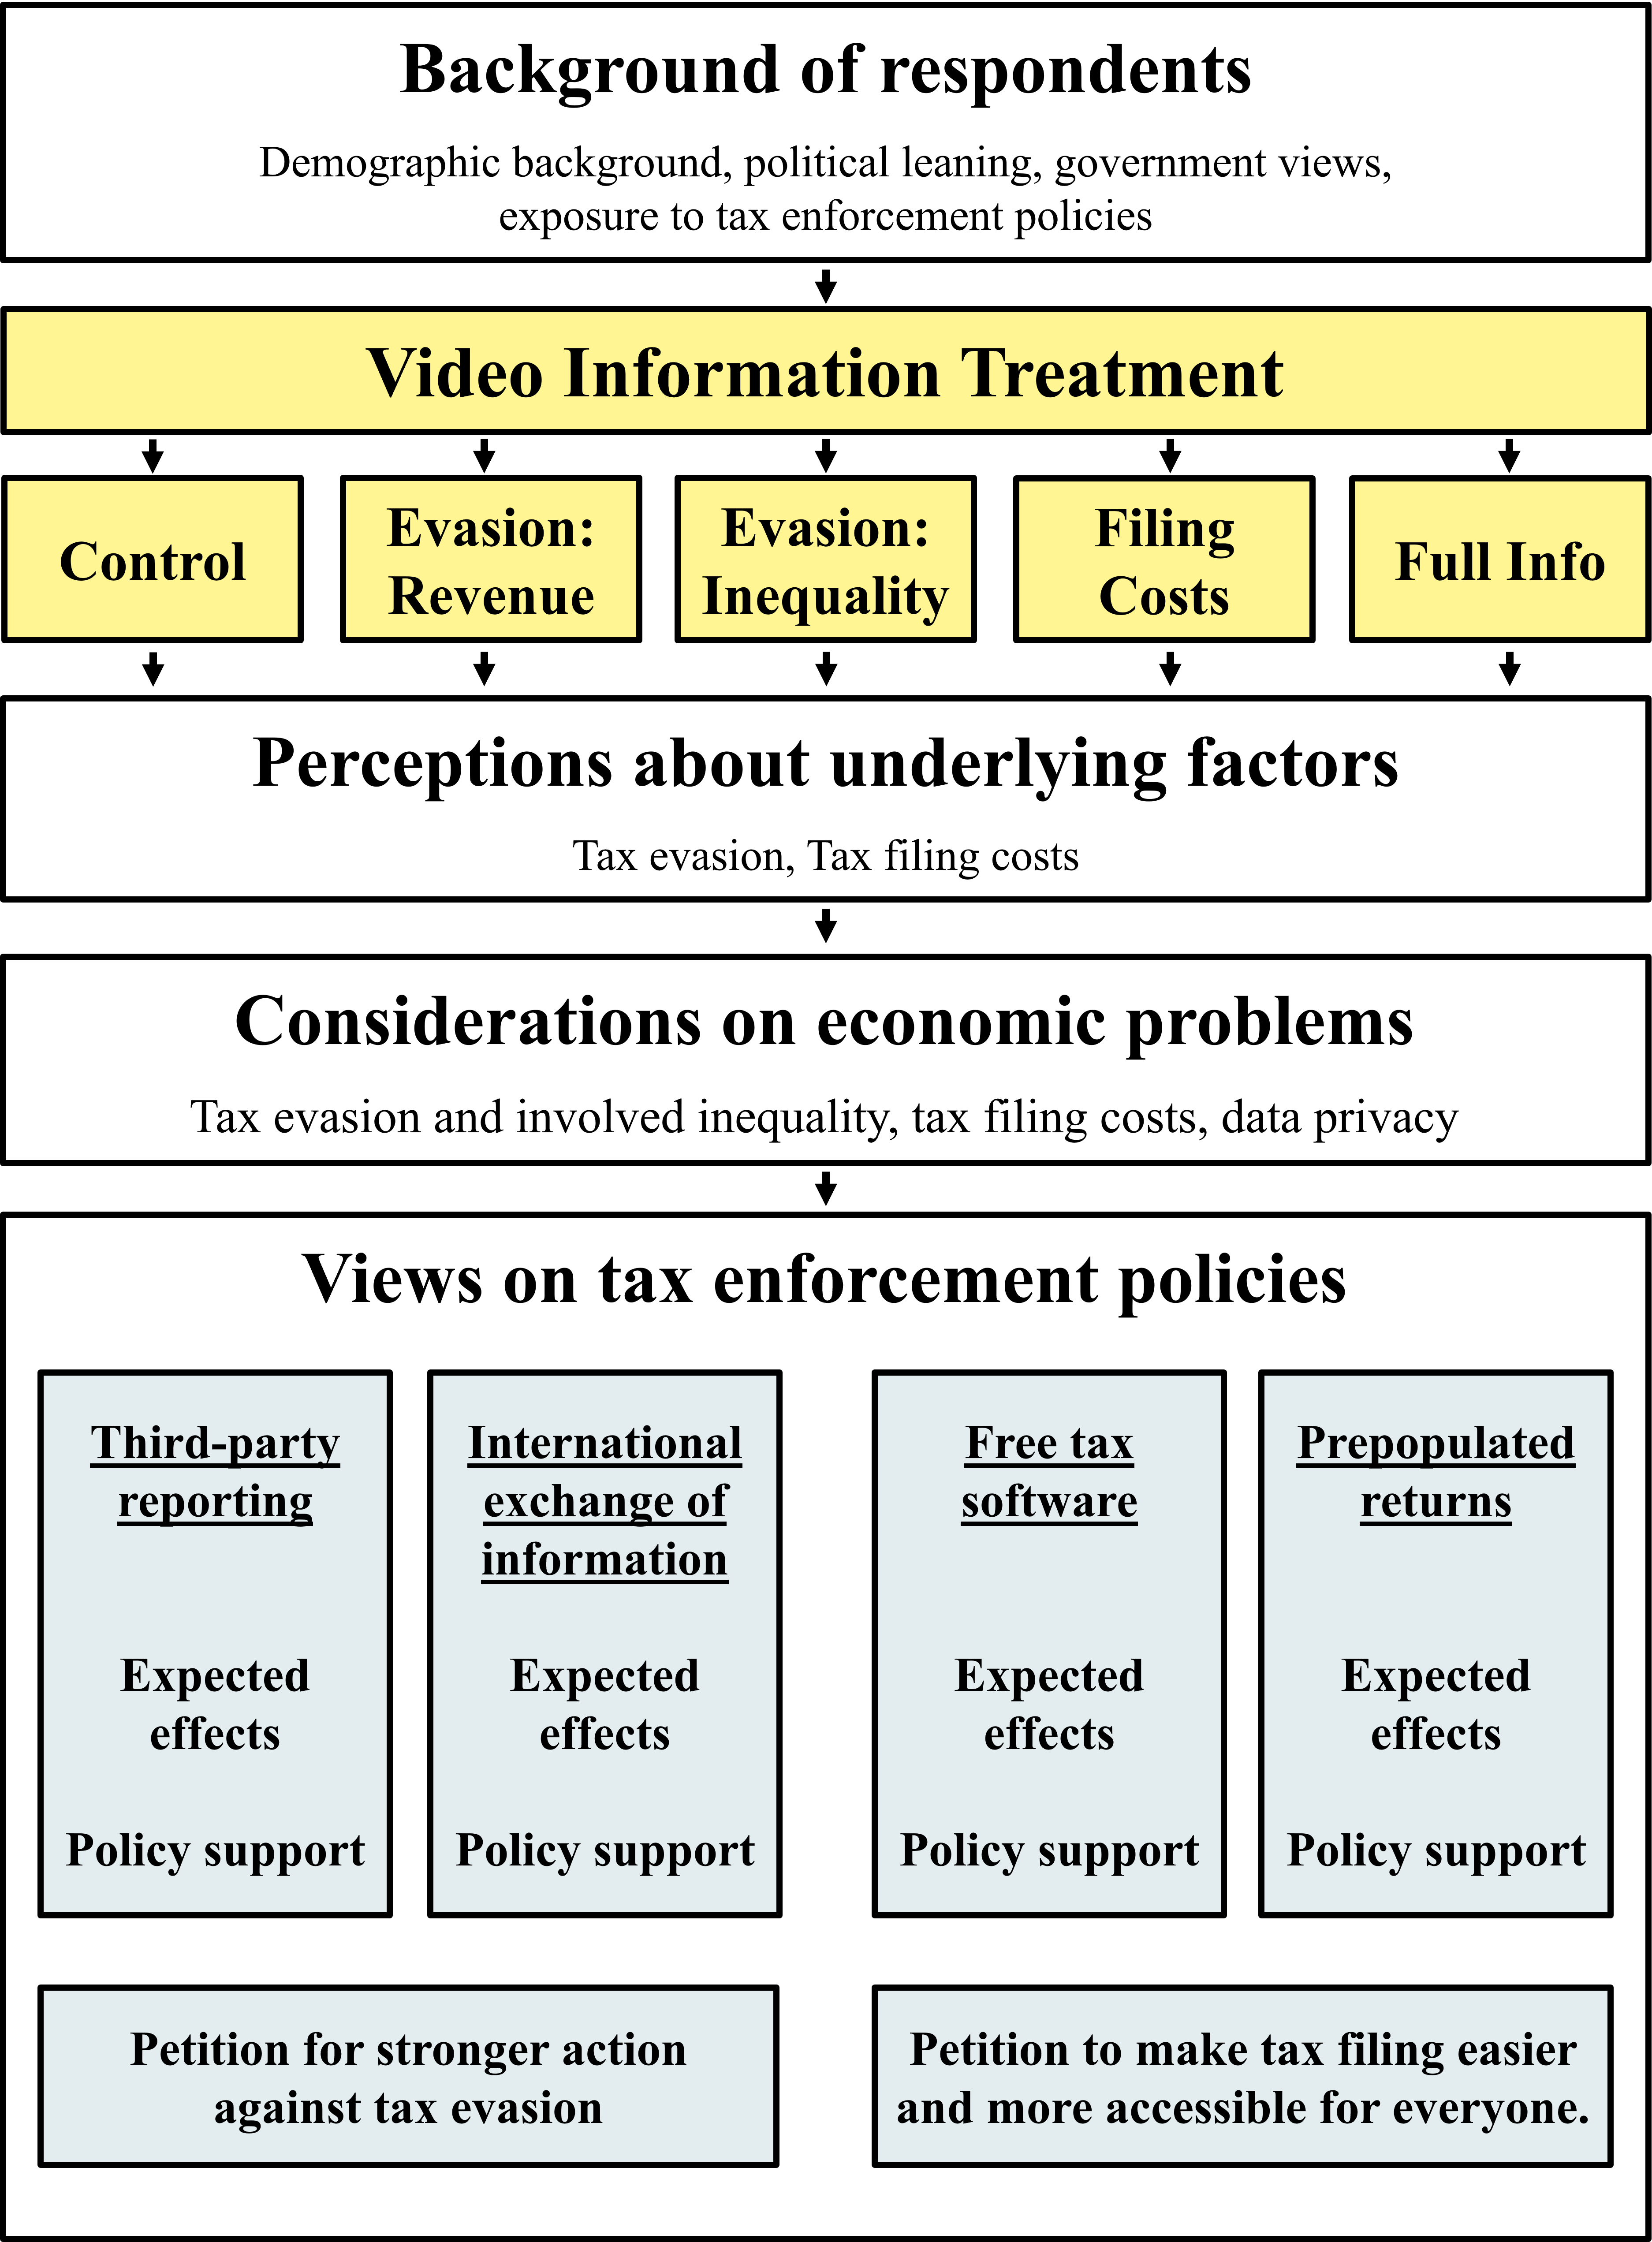
\includegraphics[width=1.05\linewidth]{Figures_Slides/Survey_Overview_Treatments.png}
  \end{column}
\end{columns}
\end{frame}

\begin{frame}{3) Survey \& Estimation: Equations (1)} 
\label{equations1}
\textbf{To analyze general support for policies} (TPR: Third-Party Reporting, IEI: International Exchange of Information, TS: Tax Software, PPR: Pre-Population of Tax Returns), we run regressions according to Eq.~\eqref{eq:TPR_Support}-\eqref{eq:Support_PPR}, where $\alpha$ is the intercept, $\mathbf{T_i}$ is a vector indicating the treatment arm, and $\mathbf{X}_{i}$ is a vector of control variables.\footnote[5]{For $\mathbf{X}_{i}$ we use three specifications, without controls ($\mathbf{X}_{i} = \{\}$), with only demographic controls ($\mathbf{X}_{i} = \mathbf{X}_{i}^{D}$), and one with a robust set of controls including in addition variables containing views on government and inequality, and exposure to tax enforcement/administration ($\mathbf{X}_{i} = \mathbf{X}_{i}^{R}$).}\textsuperscript{,}\footnote[6]{We follow the same approach to analyze perceptions, considerations on underlying economic problems, and expected effects of policies.}
\vspace{-0.5cm}
\begin{center}
\begin{align}
\label{eq:TPR_Support}
        \text{$TPR\_Support_{i1}$} 
    &= \alpha + \boldsymbol{\gamma}^{\top}\mathbf{T}_i + \boldsymbol{\beta}^{\top}\mathbf{X}_{i} + \varepsilon_{i} \\[0.25em]
    \label{eq:IEI_Support}
        \text{$IEI\_Support_{i}$} 
    &= \alpha + \boldsymbol{\gamma}^{\top}\mathbf{T}_i + \boldsymbol{\beta}^{\top}\mathbf{X}_{i} +  \varepsilon_{i} \\
        \label{eq:Support_TS}
    \text{$TS\_Support_i$} 
    &= \alpha + \boldsymbol{\gamma}^{\top}\mathbf{T}_i + \boldsymbol{\beta}^{\top}\mathbf{X}_{i} + \varepsilon_{i} \\[0.25em]
    \label{eq:Support_PPR}
    \text{$PPR\_Support_i$} 
    &= \alpha + \boldsymbol{\gamma}^{\top}\mathbf{T}_i + \boldsymbol{\beta}^{\top}\mathbf{X}_{i} +  \varepsilon_{i} 
\end{align}
\end{center}
\hfill \hyperlink{Controlvariables}{\beamergotobutton{Control Variables}} \hyperlink{Example:PolicySupportGen}{\beamergotobutton{Figures}}
\end{frame}

\begin{frame}{3) Survey \& Estimation: Equations (2)} 
\label{equations2}
Using the reported support measures from three different questions, \textbf{we analyze how support changes if the policy fulfills certain conditions.} To measure deviations from general support, we run a regression according to Equation~\ref{eq:TPR_Support_Conditional}, where %$\alpha$ is the intercept, $\mathbf{T_i}$ is a vector indicating the treatment arm, $\mathbf{X}_{i} = \{\}$, $\mathbf{X}_{i} = \mathbf{X}_{i}^{D}$, or  $\mathbf{X}_{i} = \mathbf{X}_{i}^{R}$ is a vector with control variables, 
$\mathbf{D}_c^{TPR}$ is a vector consisting of $k$ dummies $\mathbf{C}_k^{TPR}$, whereas for $k>1$ $\mathbf{C}_k^{TPR}=1$ if $k=c$ and $\mathbf{C}_k^{TPR}=0$ if $k \neq c$.\footnote[7]{That is, we have a panel structure, where participants are indexed by $i=1,\ldots,N$ and the type of support for which is being asked is indexed by $c=1,\ldots,9$ (1: general support, 2-9: conditional support). We include dummies $\mathbf{C}_2^{TPR},\ldots, \mathbf{C}_9^{TPR}$ which are equal to one if the support is measured under a certain condition $2,\ldots,9$.}
\vspace{-0.5cm}
\begin{center}
\begin{align}
    \label{eq:TPR_Support_Conditional}
    \text{$TPR\_Support_{ic}$}
    &= \alpha + \boldsymbol{\gamma}^{\top}\mathbf{T}_i + \boldsymbol{\delta}^{\top}\mathbf{D}_c^{TPR}+ \boldsymbol{\beta}^{\top}\mathbf{X}_{i} + \varepsilon_{ic}
\end{align}
\end{center}
\vfill
\hfill \hyperlink{Example:PolicySupportCond}{\beamergotobutton{Figures}} 
\end{frame}

\begin{frame}{3) Survey \& Estimation: Equations (3)} 
\label{equations3}
\textbf{To analyse main drivers of suppport} we run regressions according to Equations \ref{eq:TPR_driver}-\ref{eq:PPR_driver}, where $\mathbf{K}_i$ is a vector consisting of the dependent variables regarding knowledge of policies, $\mathbf{C}_i^{EP}$ is a vector consisting of the dependent variables regarding considerations on economic problems, and $\mathbf{C}_i^{TPR}$/$\mathbf{C}_i^{IEI}$/$\mathbf{C}_i^{TS}$/$\mathbf{C}_i^{PPR}$ are vectors consisting of considerations on the policy.\footnote[8]{Note that we create indices for the considerations on policies such that we only have one consideration (index) per channel. For example $\mathbf{C}_i^{TPR}$ includes \text{$TPR\_Tax\_Revenue_i^+$} which is an index for the considerations on whether TPR reduces tax evasion, whether TPR reduces administrative costs, and whether TPR increases tax revenue.}
\begin{align}
    \label{eq:TPR_driver}
    \text{$TPR\_Support_i$} 
    &= \alpha 
    + \boldsymbol{\kappa}^{\top}\mathbf{K}_i
    + \boldsymbol{\gamma}^{\top}\mathbf{C}_i^{EP} 
    + \boldsymbol{\lambda}^{\top}\mathbf{C}_i^{TPR}
    + \boldsymbol{\beta}^{\top}\mathbf{X}_i
    + \varepsilon_i \\
    \text{$IEI\_Support_i$} 
    &= \alpha 
    + \boldsymbol{\kappa}^{\top}\mathbf{K}_i
    + \boldsymbol{\gamma}^{\top}\mathbf{C}_i^{EP} 
    + \boldsymbol{\lambda}^{\top}\mathbf{C}_i^{IEI}
    + \boldsymbol{\beta}^{\top}\mathbf{X}_i
    + \varepsilon_i \\
    \text{$TS\_Support_i$} 
    &= \alpha 
    + \boldsymbol{\kappa}^{\top}\mathbf{K}_i
    + \boldsymbol{\gamma}^{\top}\mathbf{C}_i^{EP} 
    + \boldsymbol{\lambda}^{\top}\mathbf{C}_i^{TS}
    + \boldsymbol{\beta}^{\top}\mathbf{X}_i
    + \varepsilon_i \\
    \label{eq:PPR_driver}
    \text{$PPR\_Support_i$} 
    &= \alpha 
    + \boldsymbol{\kappa}^{\top}\mathbf{K}_i
    + \boldsymbol{\gamma}^{\top}\mathbf{C}_i^{EP} 
    + \boldsymbol{\lambda}^{\top}\mathbf{C}_i^{PPR}
    + \boldsymbol{\beta}^{\top}\mathbf{X}_i
    + \varepsilon_i
\end{align}    
\hfill \hyperlink{Example:PolicySupportDrivers}{\beamergotobutton{Figures}} 
\end{frame}


\begin{frame}{3) Survey \& Estimation: Open Questions } 
\label{equations5}
Pre treatment, after asking about demographics, and before asking about government views, we ask participants the following open ended questions: 
\begin{itemize}
    \item What are your main considerations, whether positive or negative, regarding the process by which U.S.\ taxpayers file their taxes? Are there any problems that the government should address? \textit{Open Ended}
    \item Now, if you think about tax evasion in the U.S., what are your main considerations that come to your mind? Are there any problems the government should address? \textit{Open Ended}\vspace{0.5em}
    \item[$\Rightarrow$] Questions address economic problems directly without priming them about one of our proposed factors.\footnote[10]{Additionally, they help us for analyzing typing speed.} \vspace{1em}
\end{itemize}
\alert{Should we include (additional) open ended questions? How should we analyze them?}

\end{frame}

%\begin{frame}{Conclusion}
%\begin{itemize}
%\item Using a survey \alert{we explore peoples' attitudes and considerations towards information-sharing and free tax filing services.} 
%\begin{itemize}
%\item Towards more comprehensive third-party reporting and international automatic exchange of information.
%\item Towards free tax software and/or prepopulated tax returns.
%\end{itemize}
%\vspace{0.5em}
%\item We include questions to \alert{uncover important drivers of policy views.}
%\begin{itemize}
%    \item Perceptions, beliefs and important considerations 
%\end{itemize}
%\vspace{0.5em}
%\item To \alert{establish causal links} between reasoning and policy views, we \alert{experimentally show} people different educational \alert{videos}.
%\end{itemize}
%\end{frame}

\begin{frame}
\centering
\vfill

{\Huge \textbf{Thank you for listening!}} \\[1.5em]

{\Large Questions and feedback to:} \\[0.5em]
\texttt{tim.kircali@unisg.ch}

\vfill
\end{frame}

\appendix

\begin{frame}{Motivation: Tax Filing Costs}
\begin{columns} % align at top
  % Left column (text)
  \begin{column}{0.5\textwidth}
  \begin{itemize}
    \item US tax payers face high \alert{tax filing costs} and are urged to buy commercial tax software to file tax returns.
    \vspace{1em}
    \item \alert{Efforts to introduce free IRS software and prepopulated tax returns repeatedly blocked.} 
    \vspace{1em}
    \item Main arguments against government provided filing services are \alert{data privacy concerns and overreach of the federal government.}
  \end{itemize}
  \end{column}

  % Right column (figure)
  \begin{column}{0.5\textwidth}
  \begin{center}
    \fbox{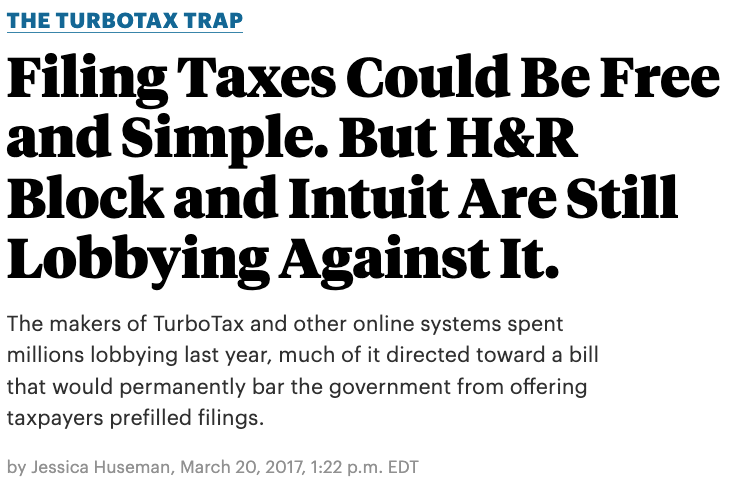
\includegraphics[width=0.9\linewidth]{Figures_Slides/Screenshot_News.png}} 

    \vspace{1.5em} % space between first and second

    \fbox{
\includegraphics[width=0.9\linewidth]{Figures_Slides/Article2.png}} 

    \vspace{0.2em} % space between second and third

    \fbox{
\includegraphics[width=0.9\linewidth]{Figures_Slides/Article_3_1.png}} 
\end{center}
  \end{column}
\end{columns}
\end{frame}


\begin{frame}{Motivation: Tax Evasion}
\begin{enumerate}
\centering
    \item \alert{Tax evasion} is a serious problem in many countries.
    \vspace{1em}
\end{enumerate}
    %\begin{itemize}
        %\item In the U.S. \$696B (15\%) taxes are not paid on time and \$606B (13\%) are never collected. \parencite{IRS_TaxGap_2022_Pub5869} 
    %\end{itemize}
    \begin{center}
        \fbox{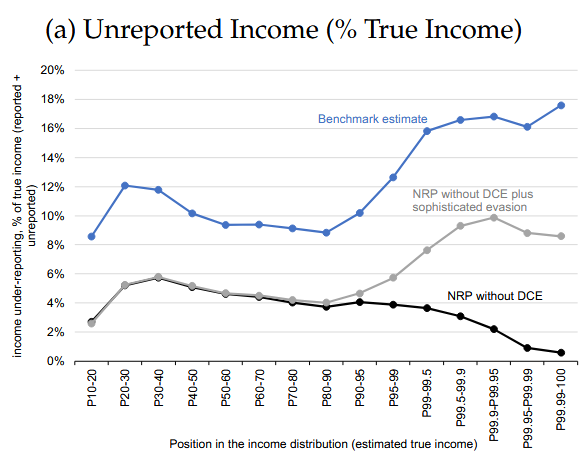
\includegraphics[width=0.45\linewidth]{Figures_Slides/Guyton.png}}
    \end{center}
    \vspace{-0.5em}
\begin{enumerate}
\centering
\setcounter{enumi}{1}
    \item Tax evasion is much \alert{more prevalent among the highest-income} earners. \parencite{guyton2021tax,alstadsaeter2019tax}
\end{enumerate}
\end{frame}

%\begin{frame}
%\frametitle{This Paper: What We Do}
%\begin{itemize}
%    \item Explores \alert{attitudes} and considerations \alert{towards information-sharing and tax filing service provision}.
%    \begin{itemize}
%        \item Towards more comprehensive third-party reporting and international automatic exchange of information. \\[0.2em]
%        \item Towards free tax software and/or prepopulated tax returns.
%    \end{itemize}
%    \vspace{1em} 
%    \item Leverages a \alert{large-scale survey to uncover considerations and beliefs} underlying these policy views.
%    \begin{itemize}
%        \item How, and why do they differ among respondents?
%    \end{itemize}
%    \vspace{1em} 
%    \item \alert{Experimental information} provision to establish \alert{causal} links between considerations and support for the policies.
%\end{itemize}
%\end{frame}
\begin{frame}
\frametitle{Two Key Rationales to Support Information-Sharing}
\begin{enumerate}
    \item Information exchange is \alert{highly effective to reduce tax evasion} \parencite{kleven2011unwilling,pomeranz2015no,slemrod2017does}
    \vspace{0.5em}
    \item The IRS needs information exchange to \alert{prepopulate tax returns}.
\end{enumerate}
\vspace{2em}
Big (!) potential: 
\vspace{0.5em}
\begin{itemize}
    \item In the U.S.\ \$696B (15\%) taxes are not paid on time and \$606B (13\%) are never collected \parencite{IRS_TaxGap_2022_Pub5869}.
    \vspace{0.5em}
    \item An average individual taxpayer has 13 hours and about \$250 tax filing costs \parencite{IRS2022}. This reflects a total cost of approximately \$100 billion per year. 
\end{itemize}
\end{frame}

\begin{frame}
\frametitle{Questions}
Should the U.S.\ adopt more comprehensive information exchange? 
\begin{itemize}
    \item \cite{boning2025welfare}: Stronger tax enforcement is welfare increasing in the U.S.\ (here by tax audits).
    \item \cite{kleven2011unwilling,pomeranz2015no,slemrod2017does}: Information sharing is highly effective to enforce taxes. 
\end{itemize}
\vspace{1em}
Should the U.S.\ offer free tax software and prepopulated tax returns?
\begin{itemize}
    \item Tax filing costs are high. (\cite{IRS2022}) \\[0.2em]
    \item Many other countries already offer these services.
\end{itemize}
\vspace{1em}
\begin{itemize}
    \item[$\Rightarrow$] \alert{Research generally says yes to policies.} 
    \item[$\Rightarrow$] \alert{But what do people think about them?}
\end{itemize}
\end{frame}

\begin{frame}{Survey to Measure (and Understand!) Policy Support }
\begin{columns}[T] % align columns at the top
  \begin{column}{0.5\textwidth} % left side for text
    \begin{itemize}
    \item Questions addressed to uncover the "invisible"
    \begin{itemize}
        \item Knowledge \& Perceptions
        \item Considerations \& Beliefs
        \item Policy support
    \end{itemize}
    \vspace{1em} 
    \item Provide \alert{policy-related information}
    \begin{itemize}
        \item Analyze how factors and considerations shape policy support
    \end{itemize}
    \end{itemize}
  \end{column}
  
  \begin{column}{0.45\textwidth} % right side for image
    \centering
    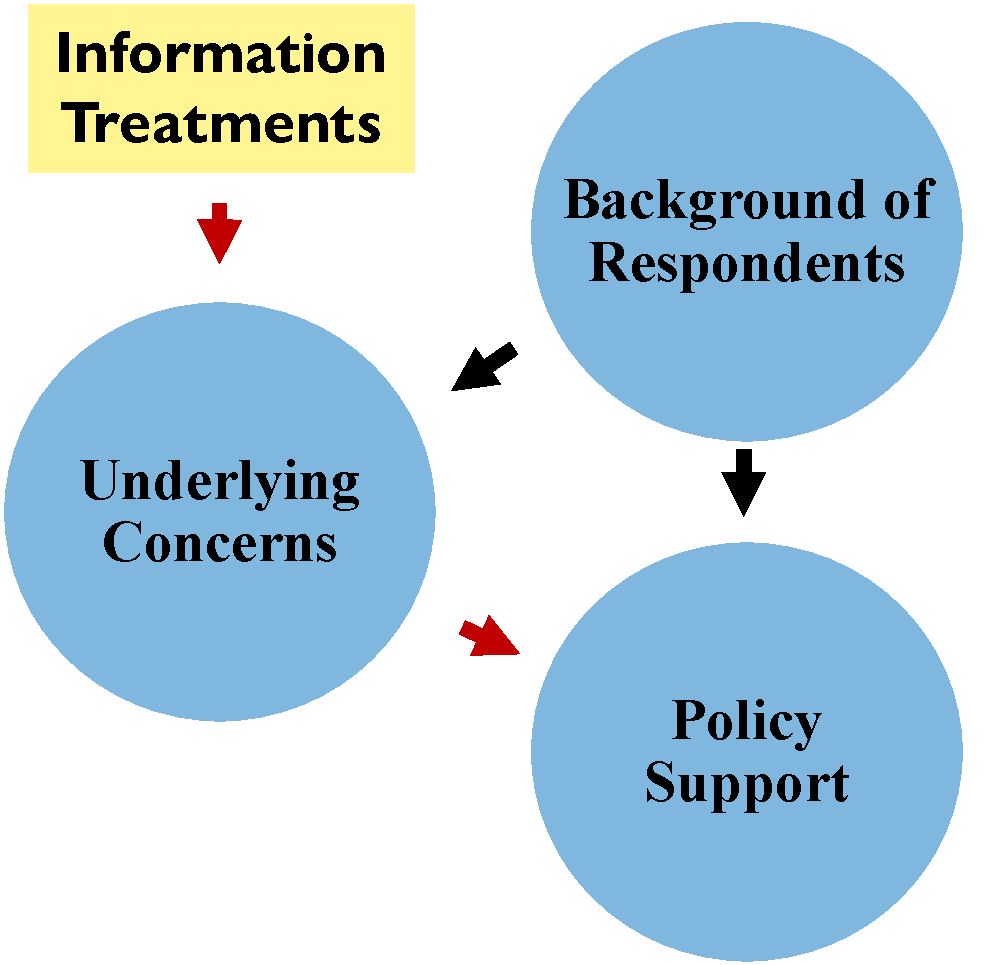
\includegraphics[width=\linewidth]{Figures_Slides/Estimation_Strategy.pdf}
  \end{column}
\end{columns}
\end{frame}

\begin{frame}{Focus on Four Considerations}
\begin{columns}[T] % align columns at the top
  \begin{column}{0.45\textwidth} % left side for text
  We concentrate on four key considerations:
  \vspace{1em}
    \begin{itemize}
        \item Tax Evasion and Government Revenue
        \vspace{0.25em}
        \item Fairness and inequality
        \vspace{0.25em}
        \item Filing Costs
        \vspace{0.25em}
        \item Data privacy
        \vspace{1em}
        \item[$\Rightarrow$] \alert{We provide respondents with information that directly addresses these considerations.}
    \end{itemize}
  \end{column}
  
  \begin{column}{0.45\textwidth} % right side for image
    \centering
     \vspace{-1em}     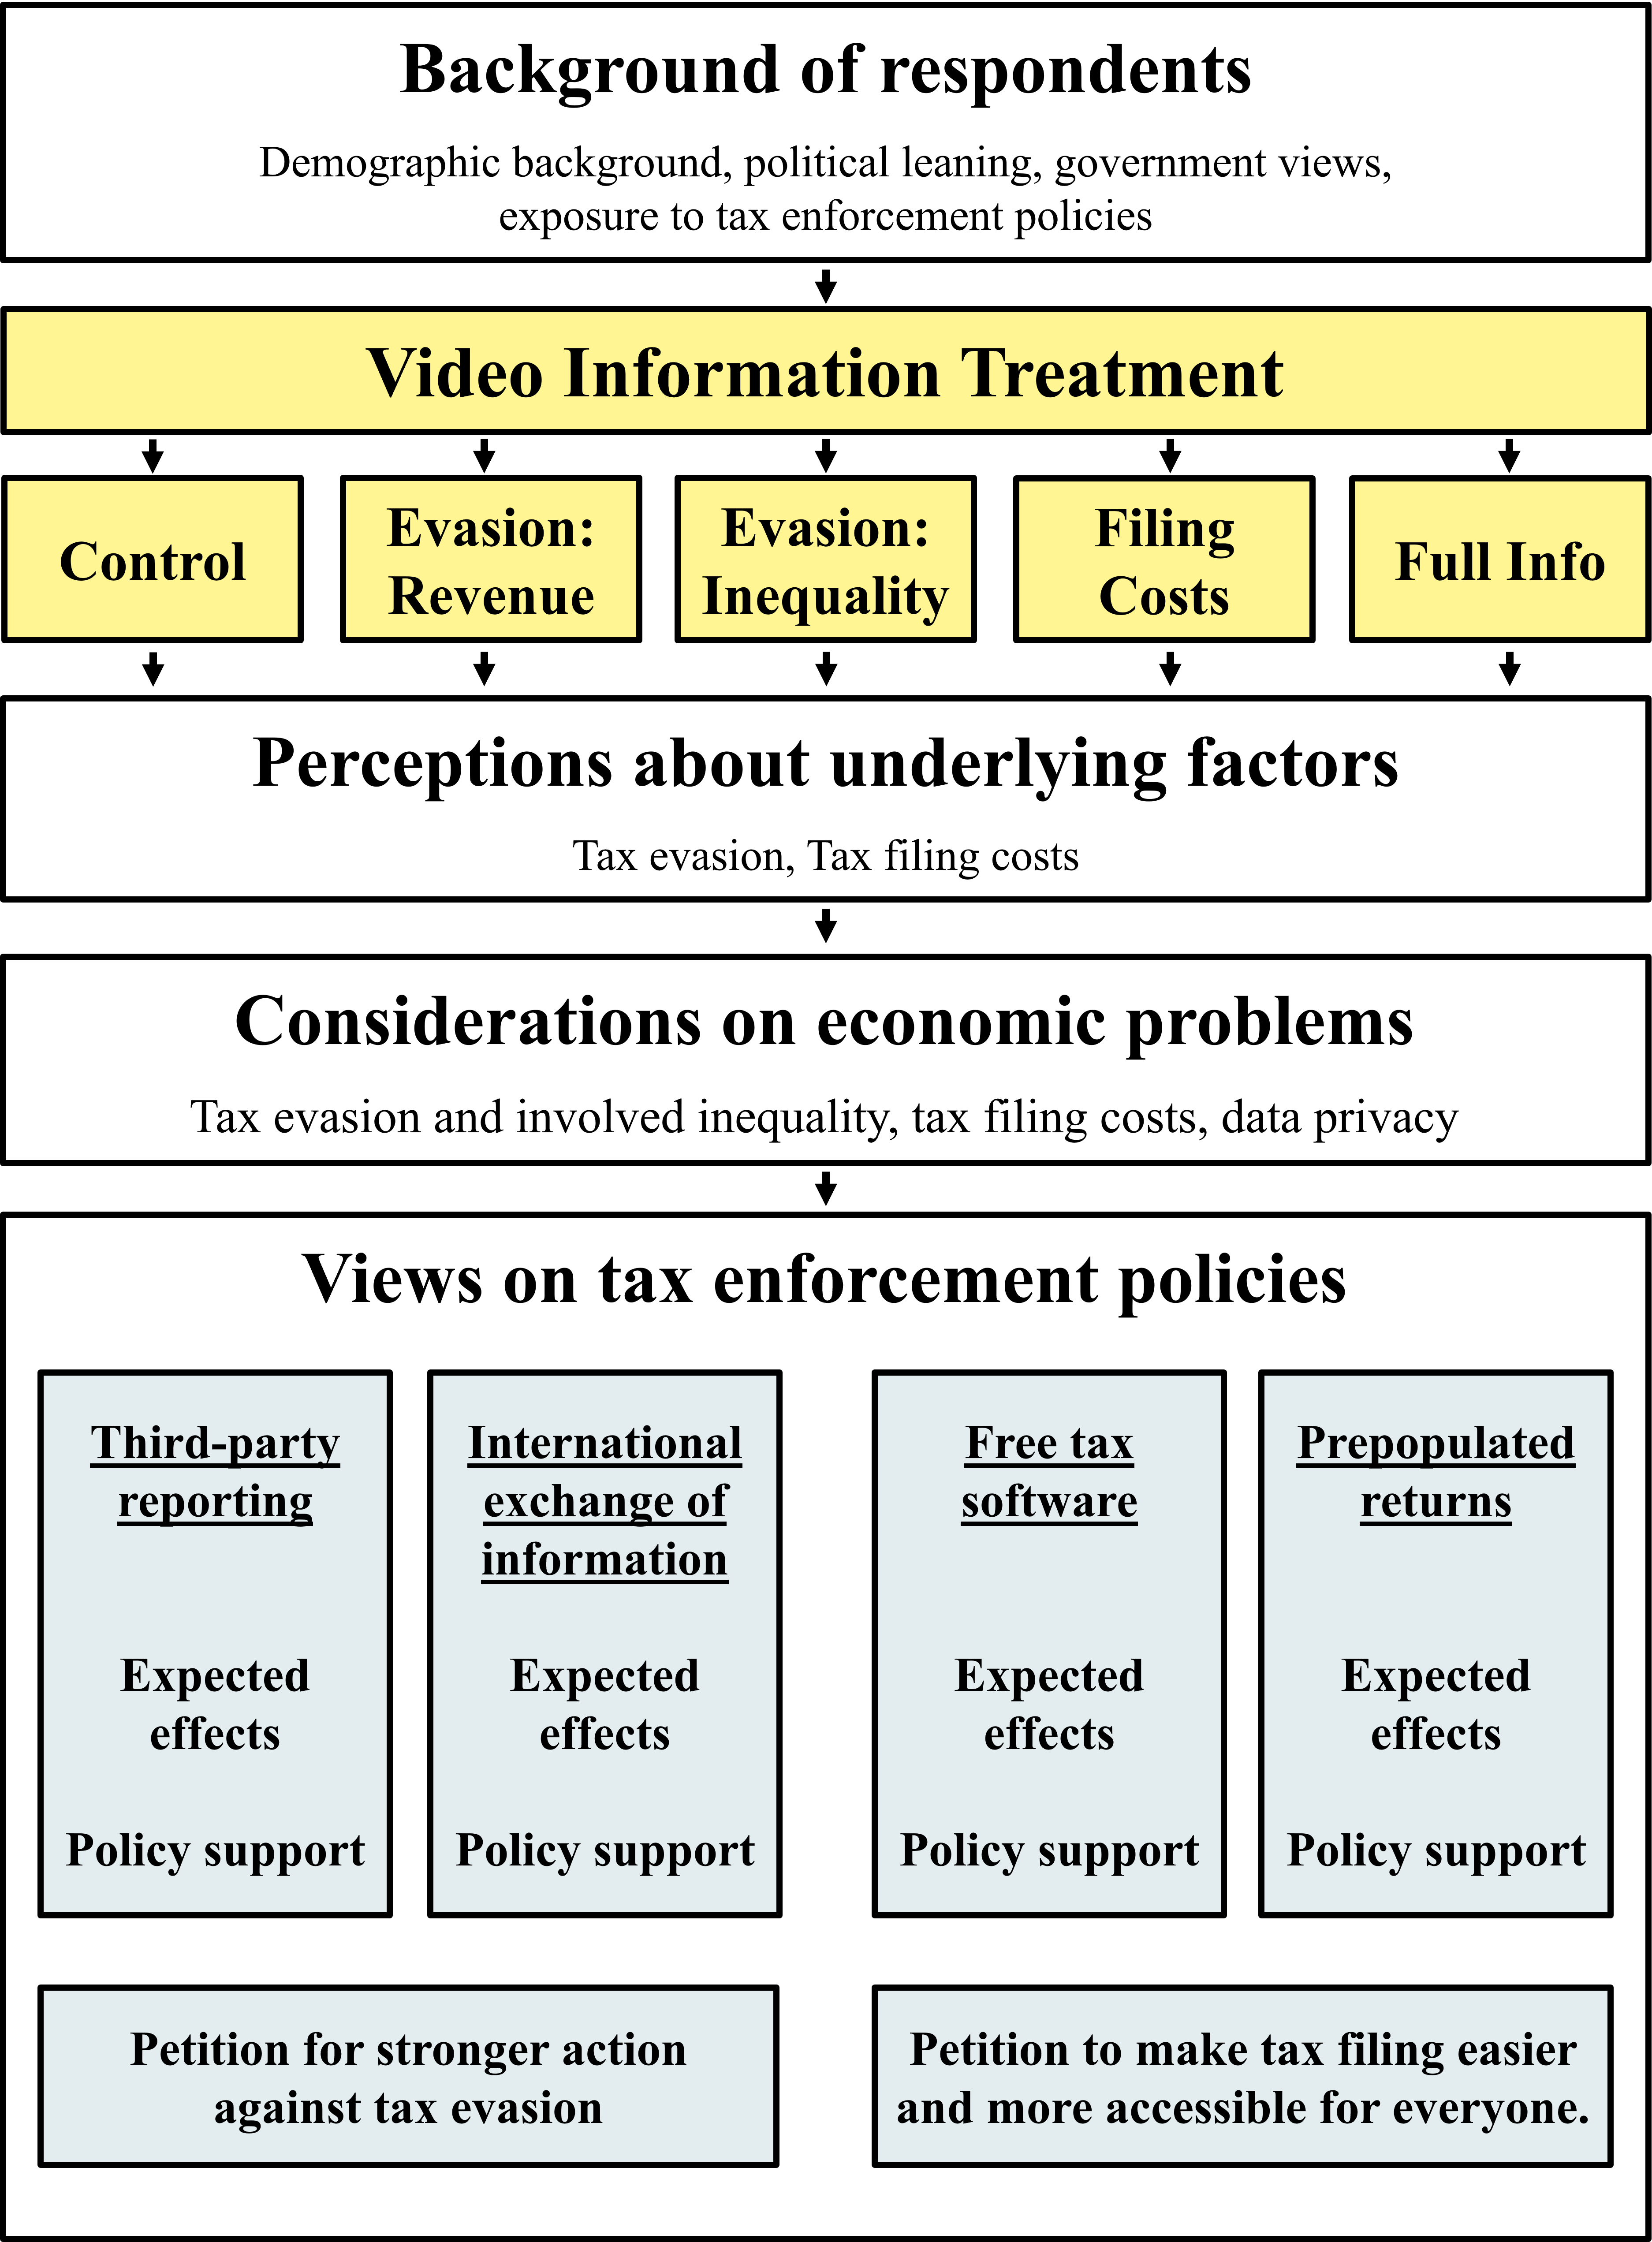
\includegraphics[width=1.05\linewidth]{Figures_Slides/Survey_Overview_Treatments.png}
  \end{column}
\end{columns}
\end{frame}
\begin{frame}
\frametitle{Related Literature}
\begin{enumerate}
    \item Measuring support for economic policies using survey experiments
\begin{itemize}
\scriptsize
    \item Tax policy: {\tiny\textcite{stantcheva2021understanding}} \\[0.1em]
    Tax simplicity and tax progressivity: {\tiny\textcite{tarroux2019value}} 
    %\item Designing information provision experiments: {\footnotesize\textcite{haaland2023designing}}\\[0.2em]  
    %Run surveys: {\footnotesize\textcite{stantcheva2023run}}.
\end{itemize}
\scriptsize
    \item[$\Rightarrow$] \alert{Measuring support for information exchange and tax filing services.}
\end{enumerate}
\begin{enumerate}
\setcounter{enumi}{1}
\item Tax evasion, tax enforcement and information reporting
\begin{itemize}
\scriptsize
    \item Third-party reporting: {\tiny \textcite{kleven2011unwilling}, \textcite{pomeranz2015no}, \textcite{kleven2016can}, \textcite{slemrod2017does}, \textcite{jensen2022employment}} \\[0.1em]
    Automatic exchange of information: {\tiny \textcite{baselgia2023compliance}, \textcite{boas2024taxing}} \\[0.1em]
    \item Distribution of tax evasion: {\tiny \textcite{johns2010distribution}, \textcite{alstadsaeter2019tax}, \textcite{guyton2021tax}}  
\end{itemize}
\scriptsize
\item[$\Rightarrow$] \alert{How do these documented facts shape policy support for information exchange?}
\vspace{0.2em} 
\end{enumerate}
\begin{enumerate}
\setcounter{enumi}{2}
\item Tax compliance costs and government's role to reduce them 
\begin{itemize}
\scriptsize
    \item Tax filing costs: {\tiny\textcite{blumenthal1992compliance}, \textcite{benzarti2020taxing}}  \\[0.1em]
    Non-filing: {\tiny\textcite{hauck2024optional}} \\[0.1em]
    Tax complexity: {\tiny\textcite{benzarti2024rising}, \textcite{tarroux2019value}}  \\[0.1em]
    \item Prepopulated tax returns: {\tiny\textcite{goodman2023automated}} \\[0.1em]
\end{itemize}
\scriptsize
\item[$\Rightarrow$] \alert{Analyse support for prepopulated tax returns and tax software (and its drivers).} 
\item[$\Rightarrow$] \alert{Explore the relation of support for tax filing services with support for information sharing.}
\end{enumerate}
\end{frame}


\section{Survey and Sample}

\begin{frame}{Recruitment and Screening}
\begin{columns}[T] % align columns at the top
  \begin{column}{0.45\textwidth} % left side for text
    \begin{itemize}
    \item U.S.\ residents aged 18 to 69 are recruited through a commercial survey company (e.g. Prolific / Bilendi)
    \vspace{1em} 
    \item \alert{Quota representativity} 
    \begin{itemize}
        \item Dimensions gender, age, region and education
    \end{itemize}
    \vspace{1em} 
    \item \alert{Avoid selection}
    \begin{itemize}
        \item Recruit without revealing topic / identity
    \end{itemize}
    \vspace{1em} 
    \item Embedded \alert{attention checks} for high-quality responses. 
    \end{itemize}
  \end{column}
  
  \begin{column}{0.45\textwidth} % right side for image
    \centering
    \vspace{-2em}
    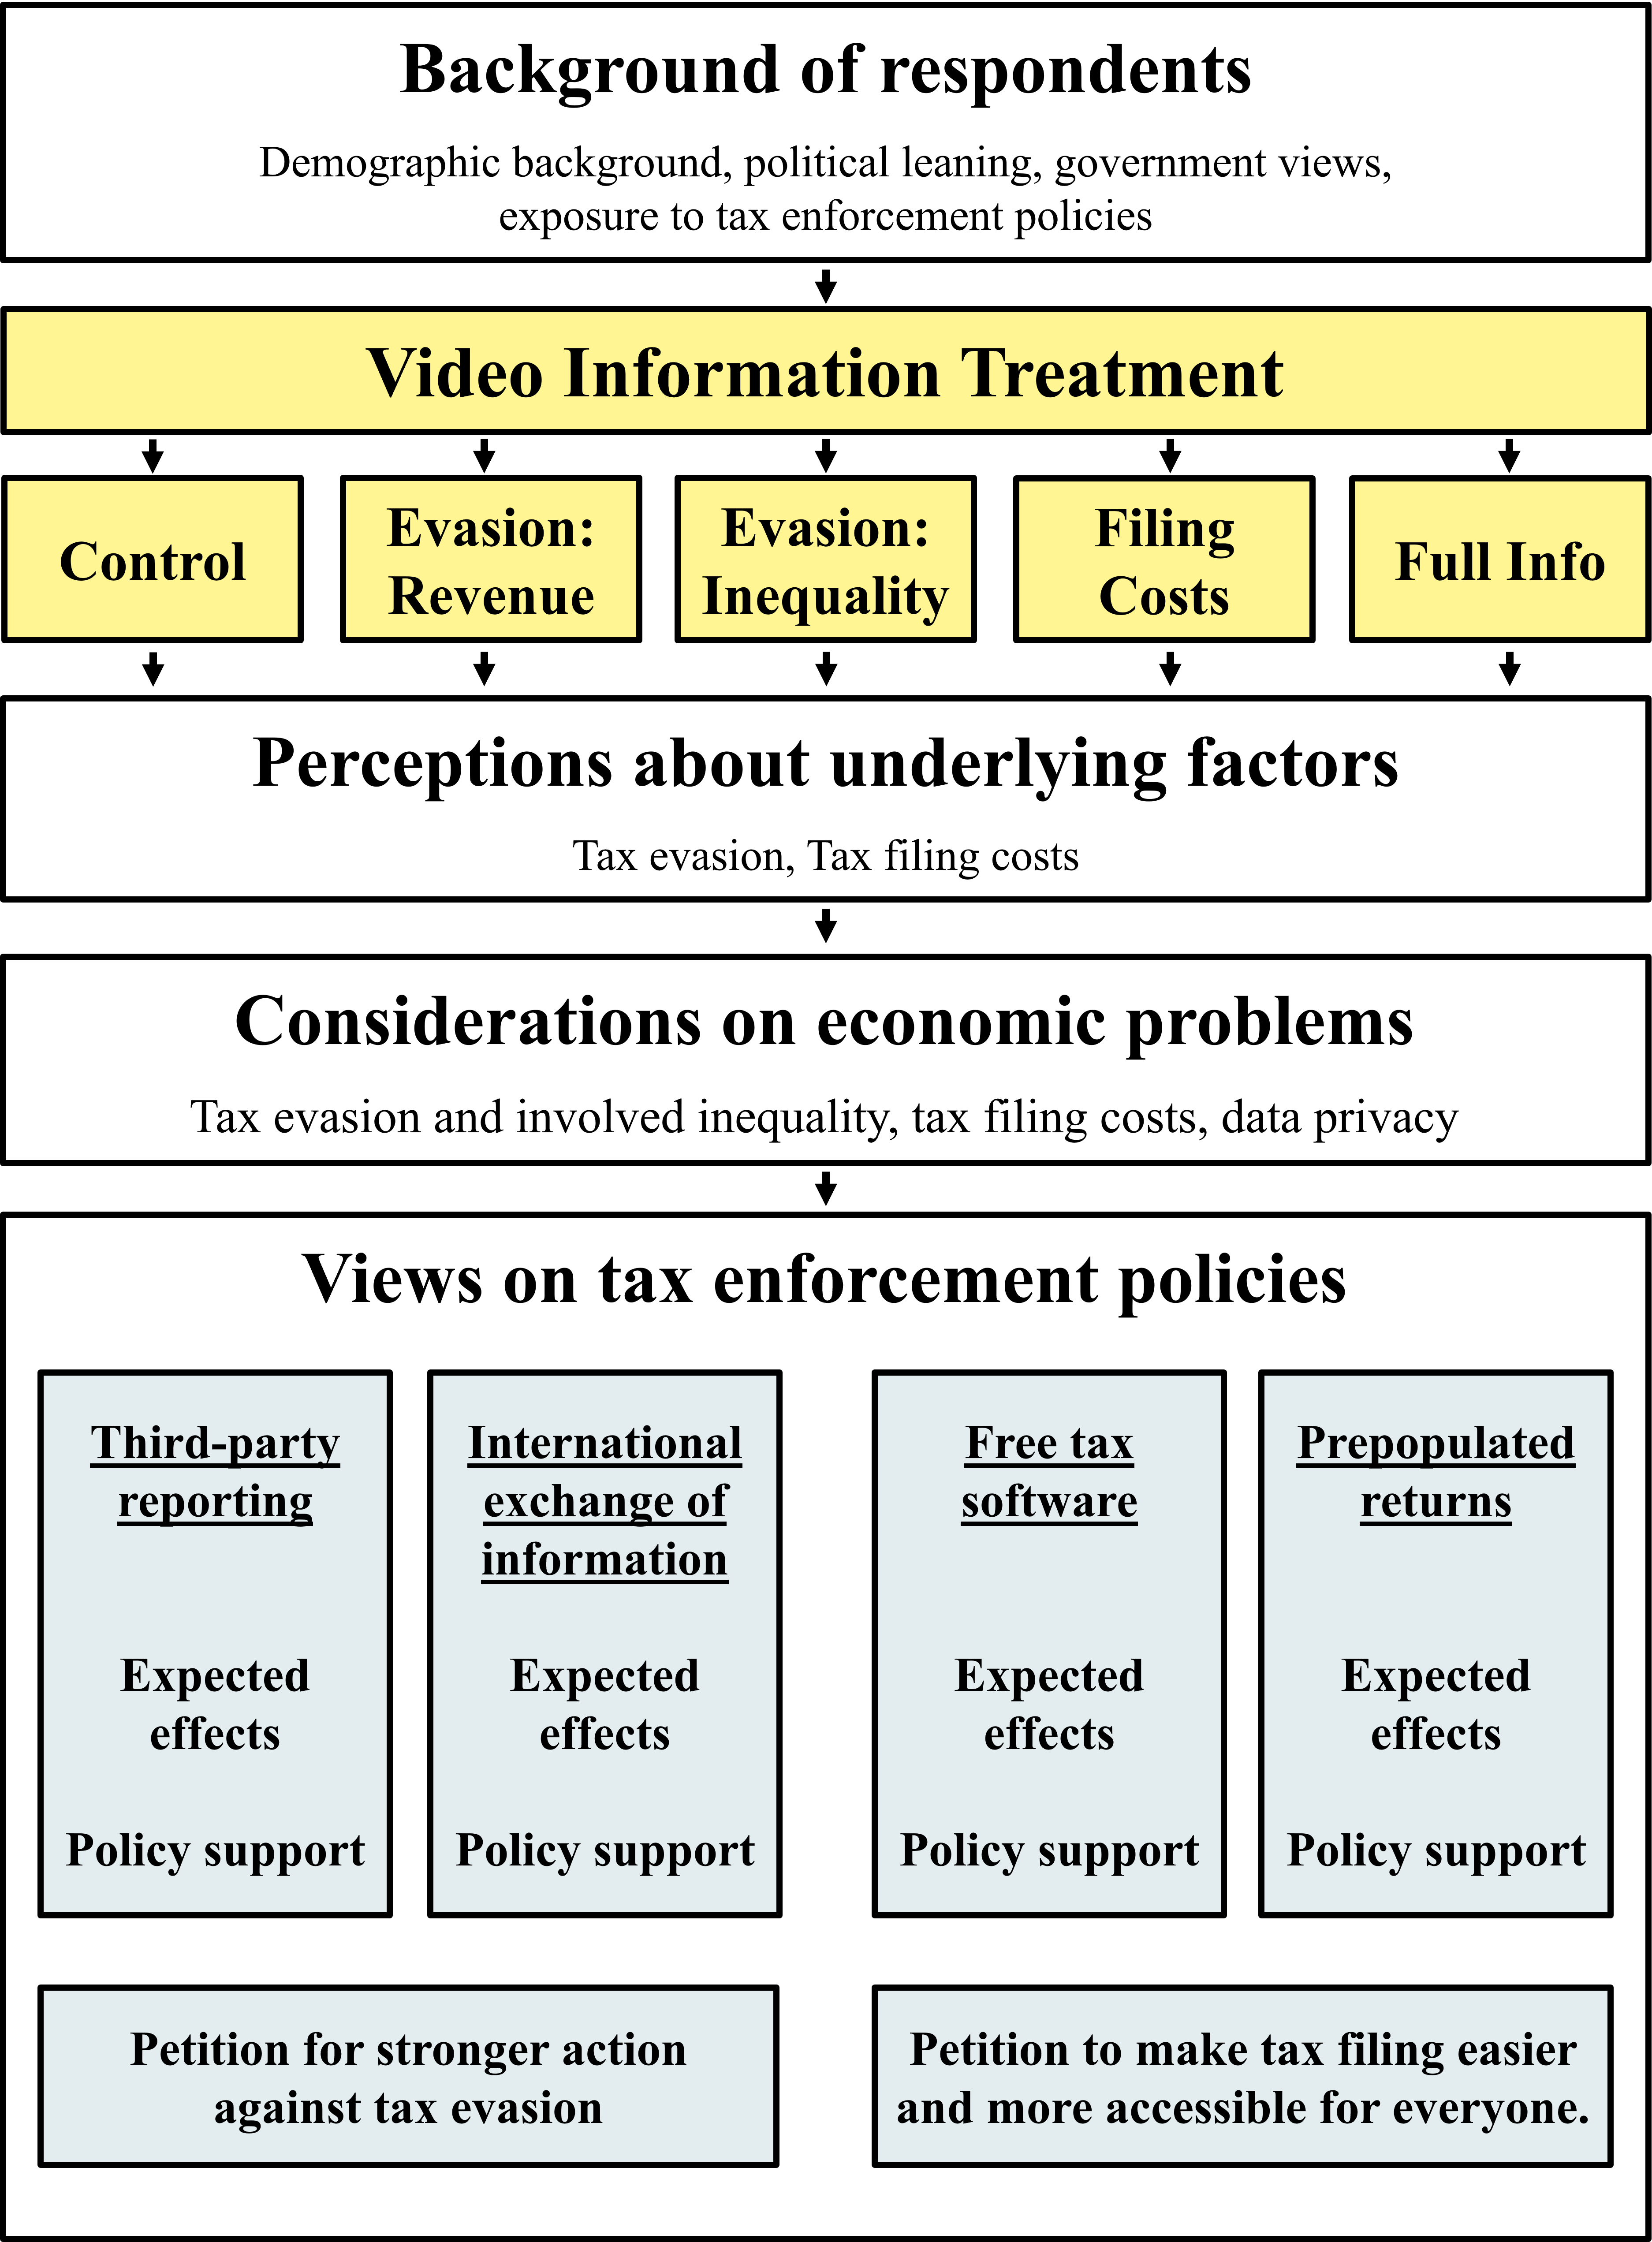
\includegraphics[width=1.05\linewidth]{Figures_Slides/Survey_Overview_Treatments.png}
  \end{column}
\end{columns}
\end{frame}

\begin{frame}{Sample and Quality}
\label{Quotas}
\begin{columns}[T] % align columns at the top
  \begin{column}{0.45\textwidth} % left side for text
  \begin{itemize}
    \vspace{2em}
      \item Recruit \alert{quota representative sample} of participants with a neutral screening page.
      \vspace{1em}
      \item Conduct several quality checks:
      \begin{itemize}
        \vspace{0.25em}
          \item Screening questions
          \begin{itemize}
              \item 2 text based
              \item 2 with audio + video
          \end{itemize}
          \vspace{0.25em}
          \item Check for attrition bias
          \vspace{0.25em}
          \item Additional Checks 
          \begin{itemize}
              \item e.g. typing speed
          \end{itemize}
          
      \end{itemize}
  \end{itemize}
  \vspace{2em}
  \hyperlink{pretreatment}{\beamergotobutton{Back: Pre Treatment}}
  \end{column}
  \begin{column}{0.45\textwidth} % left side for text
\vspace{-2.5em}
\begin{table}[!htbp]\centering
\tiny
\caption{Prolific Quotas}
\label{tab:prolificquotas}
\begin{threeparttable}
\begin{tabular}{lc}
\toprule
& (1) \\
& Quotas according to 2024 census  \\

\midrule
\textbf{Gender} \\
Female                  & 50.09 \\
Male                    & 49.91 \\[0.5em]
\textbf{Age} \\
18-29                  & 23.79 \\
30-39                  & 20.92 \\
40-49                  & 19.11 \\
50-59                  & 17.95 \\
60-69                  & 18.24 \\[0.5em]
\textbf{Income}\\
\$0-\$10,000        & 5.13 \\
\$10,000–\$15,999   & 3.81 \\
\$16,000–\$19,999   & 2.21 \\
\$20,000–\$29,999   & 6.21 \\
\$30,000–\$39,999   & 6.53 \\
\$40,000–\$49,999   & 6.68 \\
\$50,000–\$59,999   & 6.43 \\
\$60,000–\$69,999   & 6.14 \\
\$70,000–\$79,999   & 5.60 \\
\$80,000–\$89,999   & 5.05 \\
\$90,000–\$99,999   & 5.05 \\
\$100,000–\$149,999 & 17.76\\
more than \$150,000 & 23.40 \\
\bottomrule
\end{tabular}
\begin{tablenotes}[flushleft]
\item \textit{Notes}: Census data come from American Community Survey \url{https://data.census.gov/table?q=ACS+B19001}.  
\end{tablenotes}
\end{threeparttable}
\end{table}
  \end{column}
\end{columns}
\end{frame}

\begin{frame}[label=Personal_Exposure]{Background of Respondents}
\begin{columns}[T] % align columns at the top
  \begin{column}{0.45\textwidth} % left side for text
    \begin{itemize}
    \item Demographic background %(age, education, region, income, ethnicity, household composition) 
    \vspace{0.5em} 
    \item Political leaning
    \begin{itemize}
        \item Political affiliation
    \end{itemize}
    \vspace{0.5em} 
    \item Government views
    \begin{itemize}
        \item Trust
        \item Desired involvement
        \item Quality of services
    \end{itemize}
    \vspace{0.5em} 
    \item \alert{Exposure} to tax enforcement and tax administration
    \begin{itemize}
        \item Tax filing and tax software
        \item Filing mistakes and evasion
    \end{itemize}
    \end{itemize}
  \end{column}
  
  \begin{column}{0.45\textwidth} % right side for image
    \centering
     \vspace{-2em}
    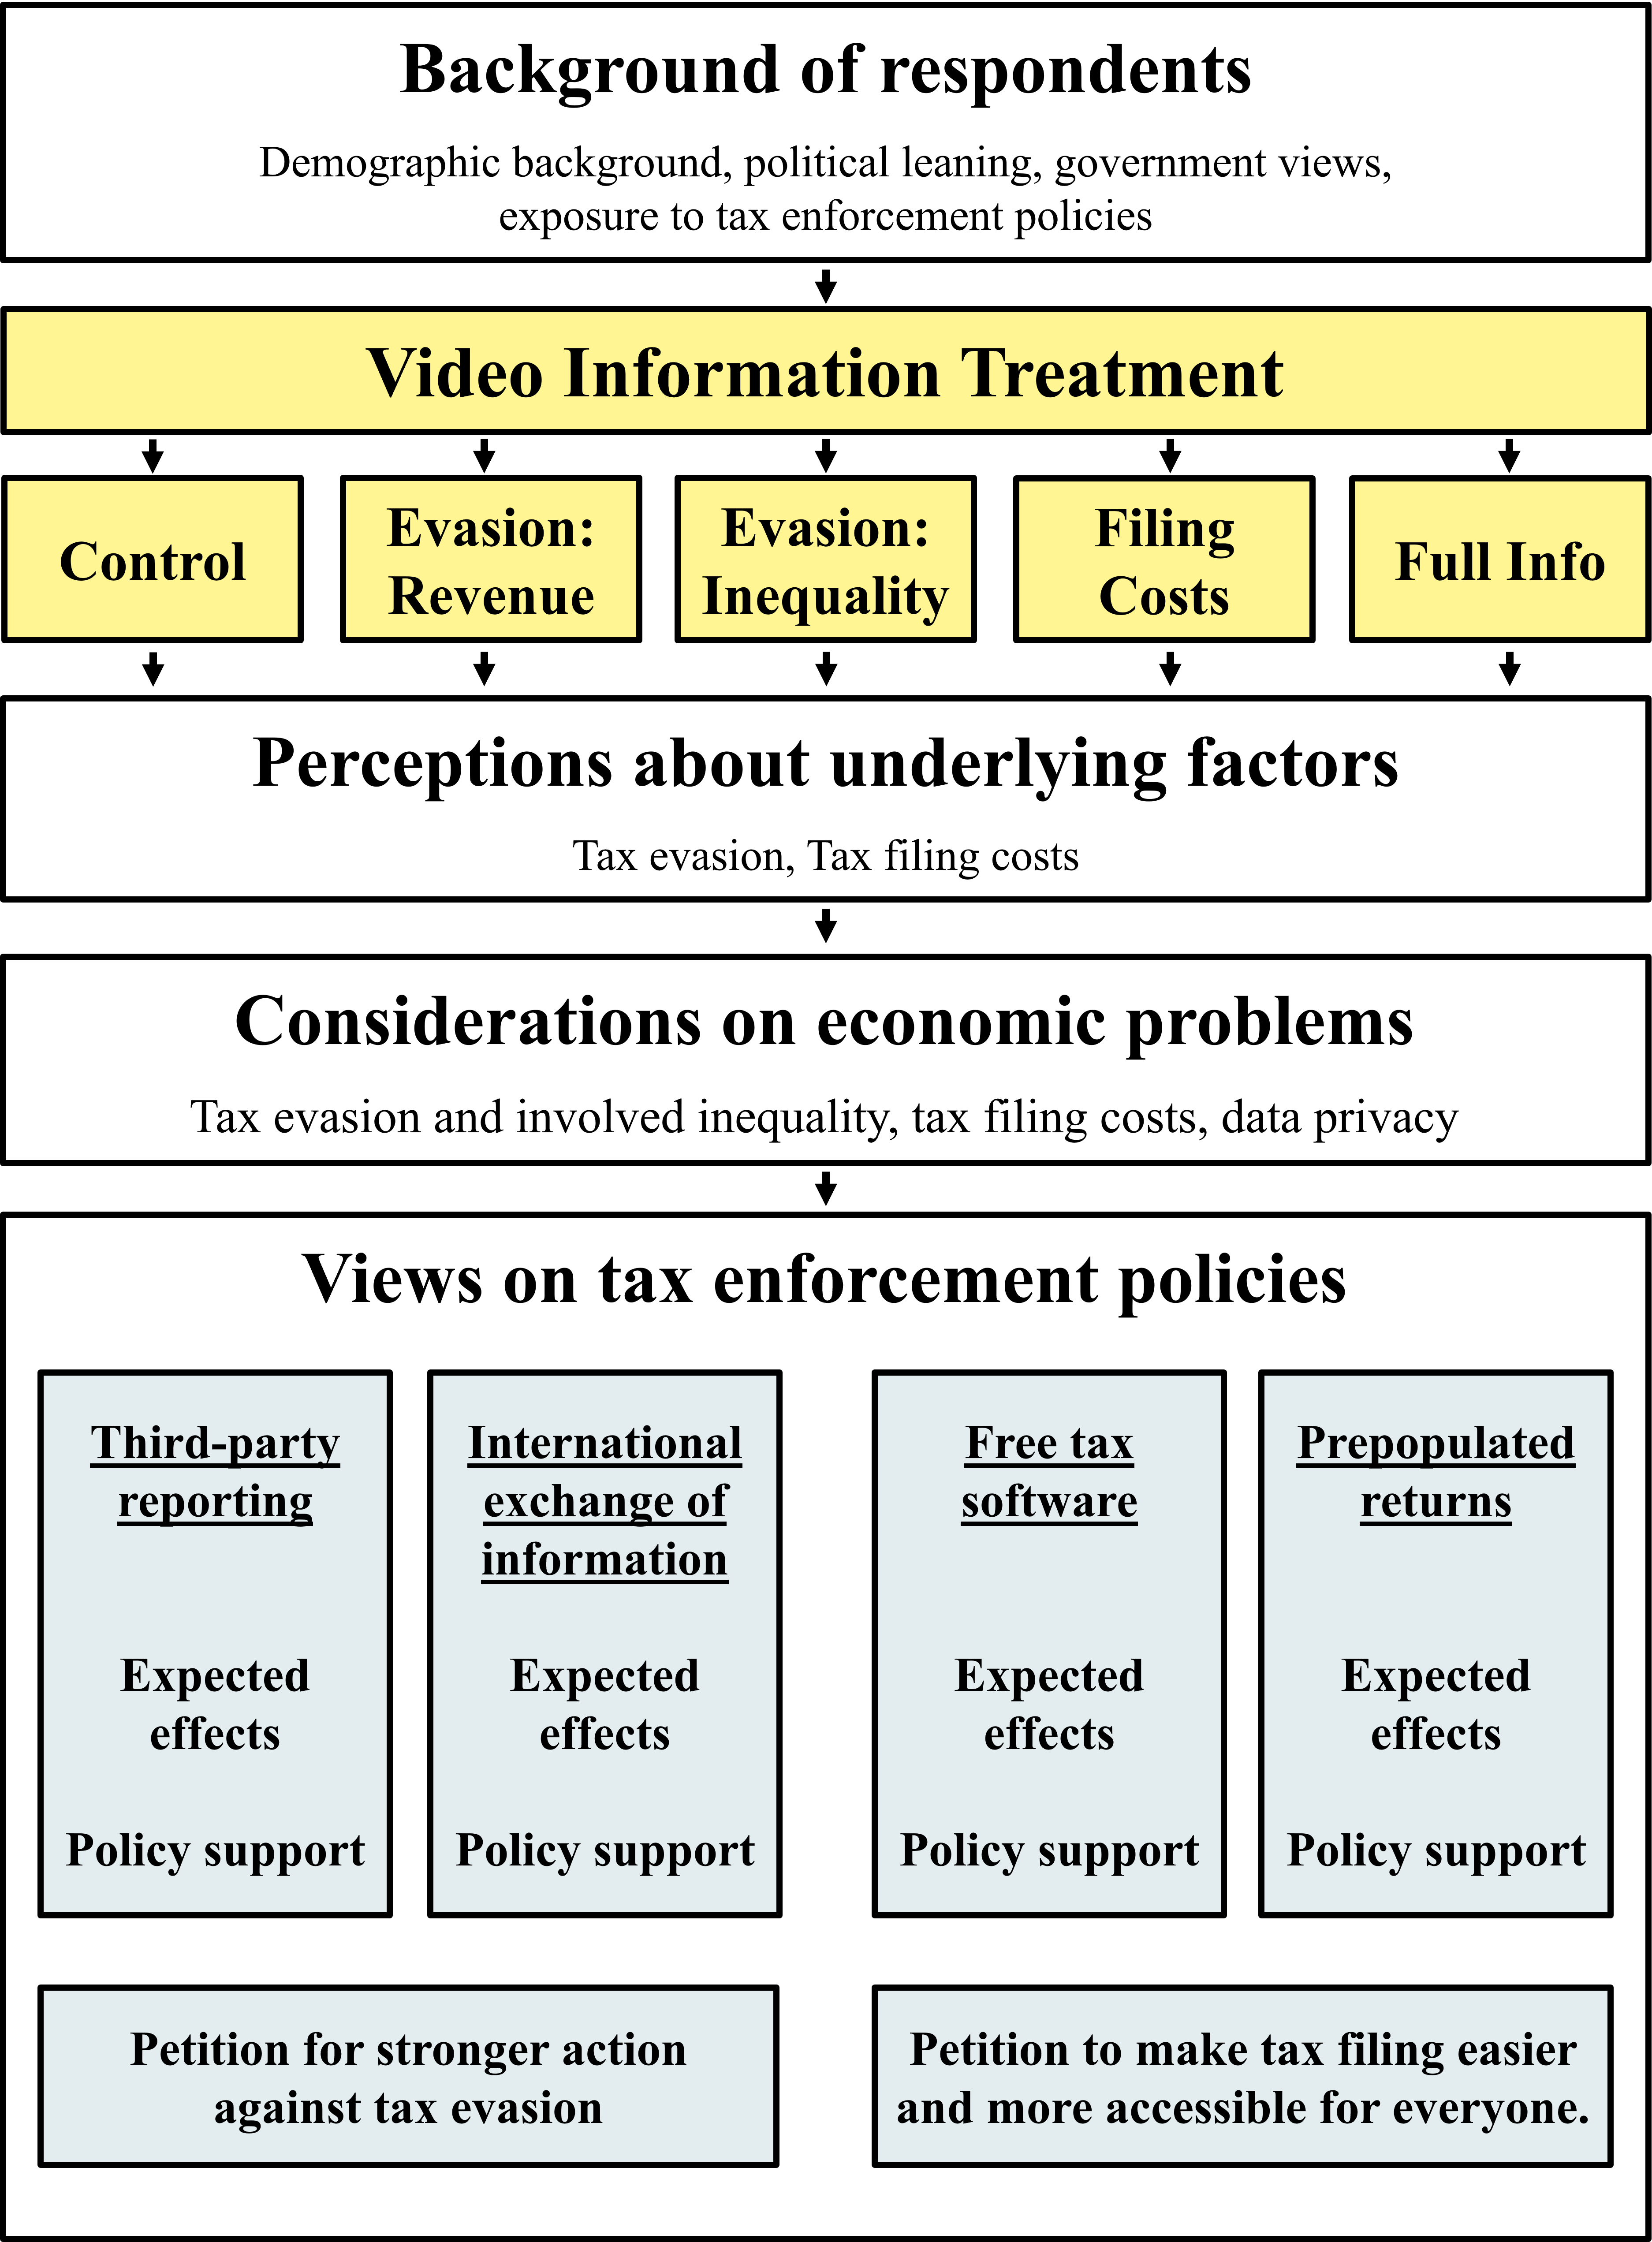
\includegraphics[width=1.05\linewidth]{Figures_Slides/Survey_Overview_Treatments.png}
  \end{column}
\end{columns}
\end{frame}

%\begin{frame}{Video Information Treatments}
%\begin{columns}[T] % align columns at the top
%  \begin{column}{0.45\textwidth} % left side for text
%    \begin{itemize}
%    \vspace{1em} 
%    \item Educational \alert{information videos}
%    \begin{itemize}
%        \item Audio
%        \item Subtitles
%        \item Animated
%    \end{itemize}
%    \vspace{1.5em} 
%    \item Close \alert{link to important underlying concerns} 
%    \begin{itemize}
%        \item Tax evasion \& revenue
%        \item Fairness \& inequality
%        \item Tax filing costs
%    \end{itemize}
%    \end{itemize}
%  \end{column}
%  
%  \begin{column}{0.45\textwidth} % right side for image
%    \centering
%     \vspace{-2em}     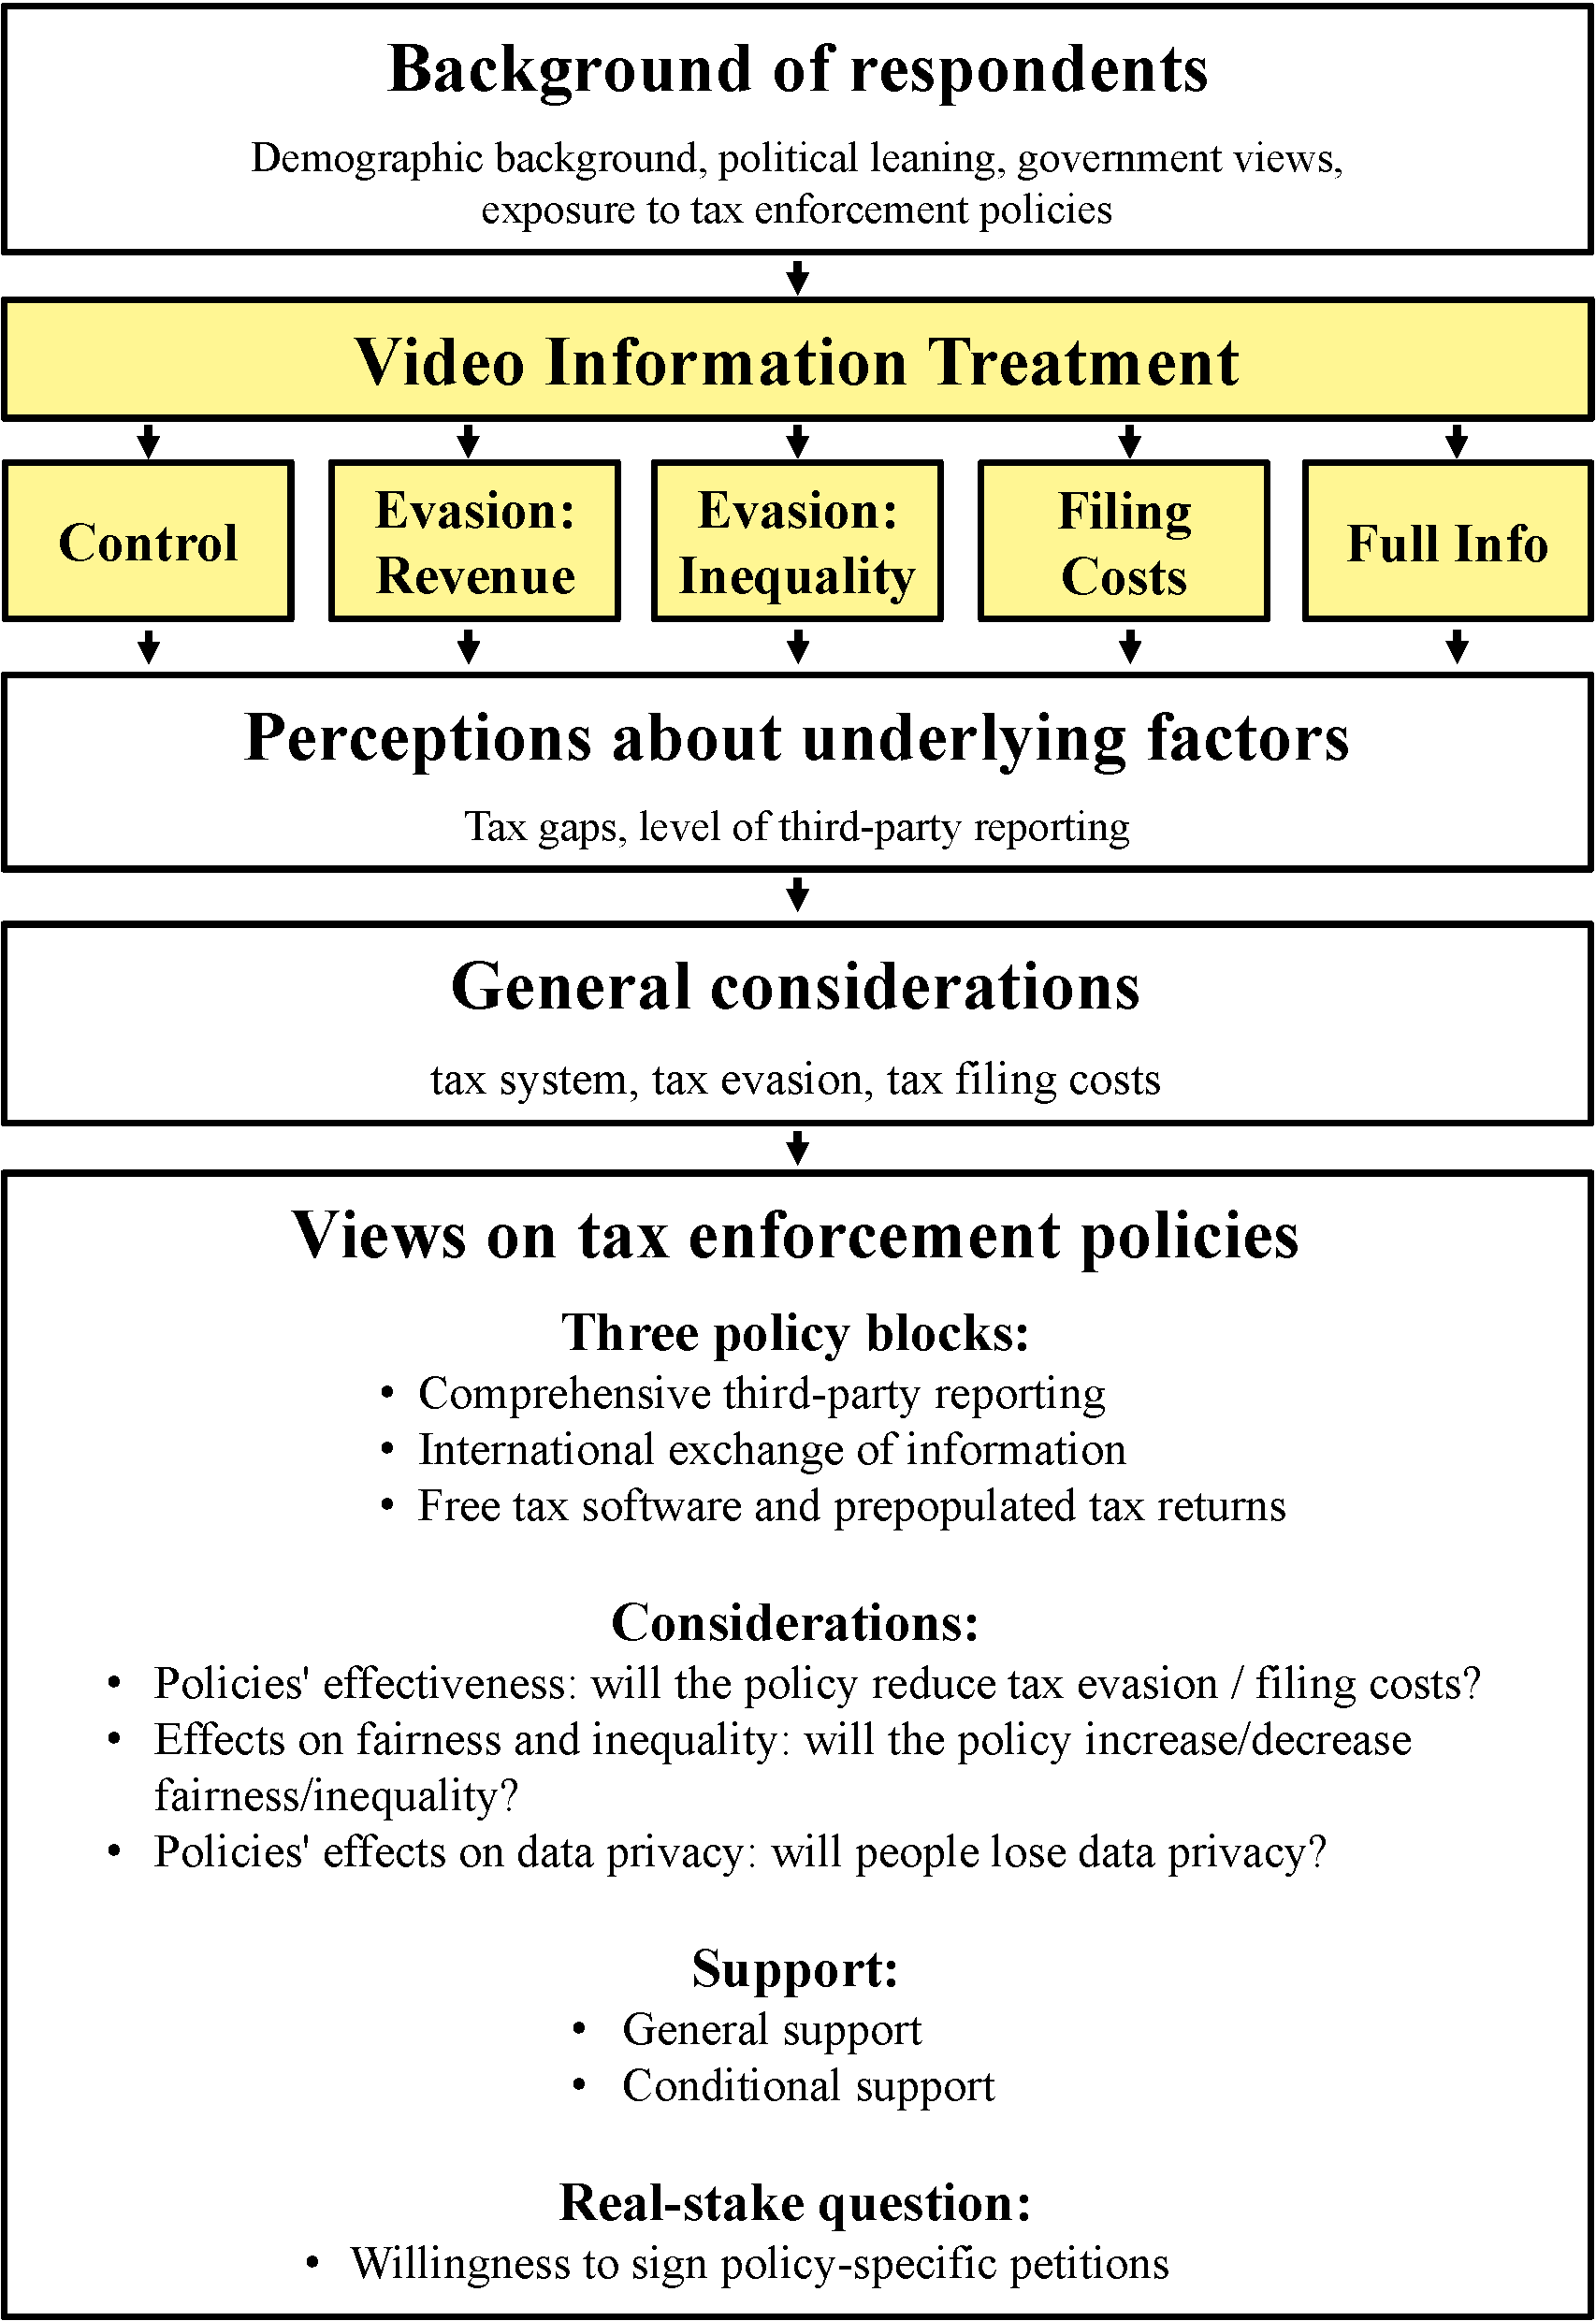
\includegraphics[width=1.05\linewidth]{Figures_Slides/Survey_Overview_Treatments.pdf}
%  \end{column}
%\end{columns}
%\end{frame}

%\begin{frame}{Video Information Treatments}
%\begin{columns}[T] % align columns at the top
%  \begin{column}{0.45\textwidth} % left side for text
%    \begin{itemize}
%    \vspace{1em} 
%    \item Educational \alert{information videos}
%    \begin{itemize}
%        \item Audio
%        \item Subtitles
%        \item Animated
%    \end{itemize}
%    \vspace{1.5em} 
%    \item Close \alert{link to important underlying concerns} 
%    \begin{itemize}
%        \item Tax evasion \& revenue
%        \item Fairness \& inequality
%        \item Tax filing costs
%    \end{itemize}
%    \end{itemize}
%  \end{column}
%  
%  \begin{column}{0.45\textwidth} % right side for image
%    %\vspace{0.3cm}
%    \centering
%    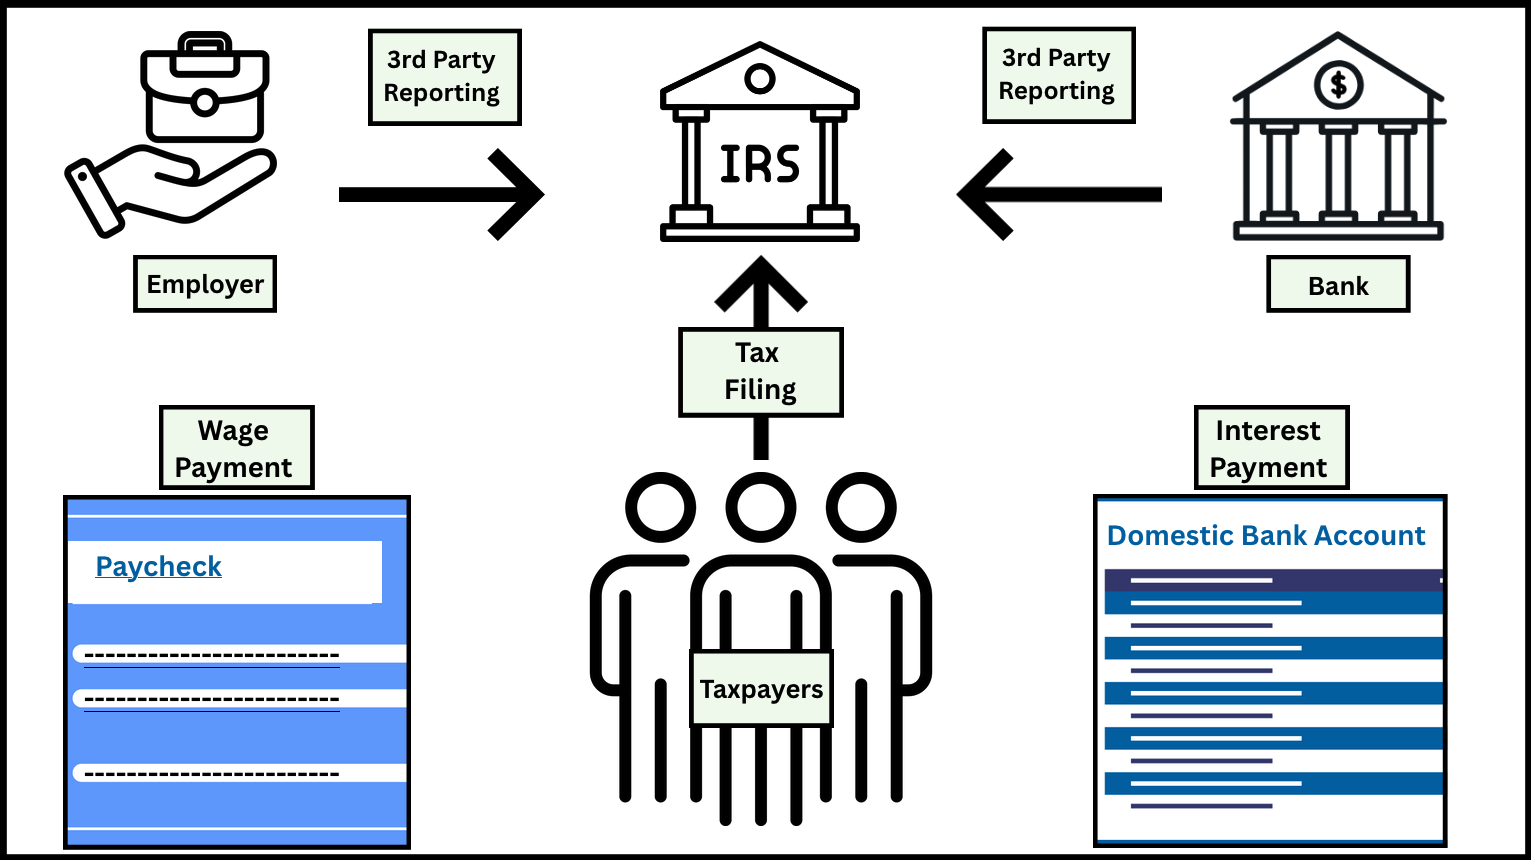
\includegraphics[width=0.95\linewidth]{Figures_Slides/Screenshot_3.png}\\[0.5cm]
%    %\vspace*{1cm}
%    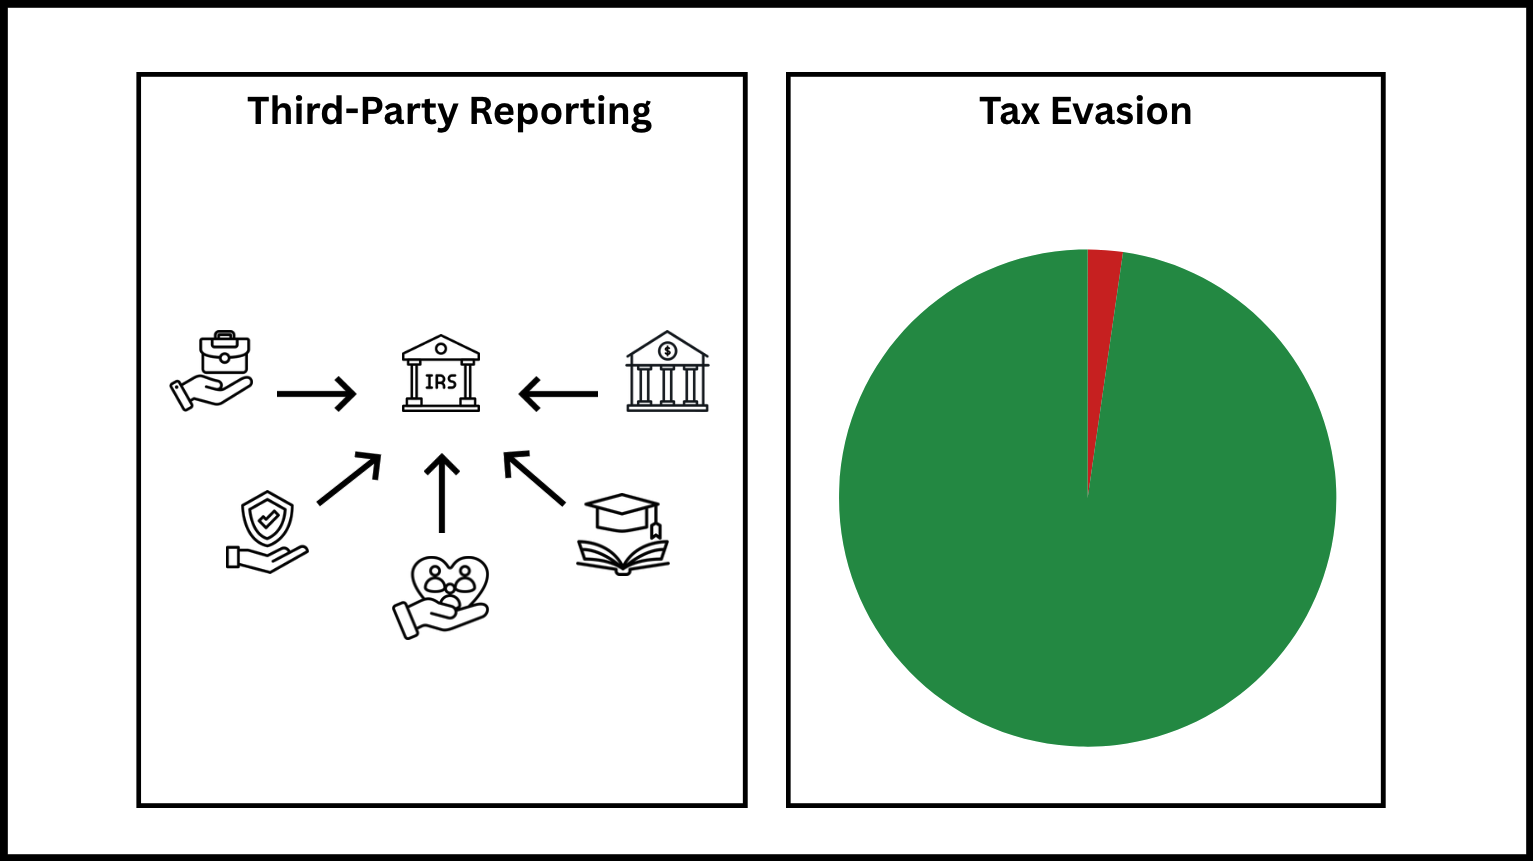
\includegraphics[width=0.95\linewidth]{Figures_Slides/Screenshot_2.png}
%  \end{column}
%\end{columns}
%\end{frame}
\begin{frame}{Evasion: Revenue}
\label{frame:Evasionrevenue}
\begin{columns}[T] % align columns at the top
  \begin{column}{0.45\textwidth} % left side for text
    \begin{itemize}
    \item Information about economic problem
    \begin{itemize}
    \vspace{0.25em}
        \item \alert{Extent} of tax evasion\footnote{\cite{IRS_TaxGap_2022_Pub5869}}
    \end{itemize}
    \vspace{2.5em} 
    \item Information about policy
    \begin{itemize}
    \vspace{0.25em}
        \item Third-party reporting \& IEoI \alert{reduces tax evasion}\footnote{ \cite{kleven2011unwilling,pomeranz2015no,kleven2016can,slemrod2017does,jensen2022employment,baselgia2023compliance,boas2024taxing}}
        \vspace{4.5em}
    \end{itemize}
    \end{itemize}
  \end{column}
  
  \begin{column}{0.45\textwidth} % right side for image
    %\vspace{0.3cm}
    \centering
    \vspace{-0.5em}
    \fbox{%
  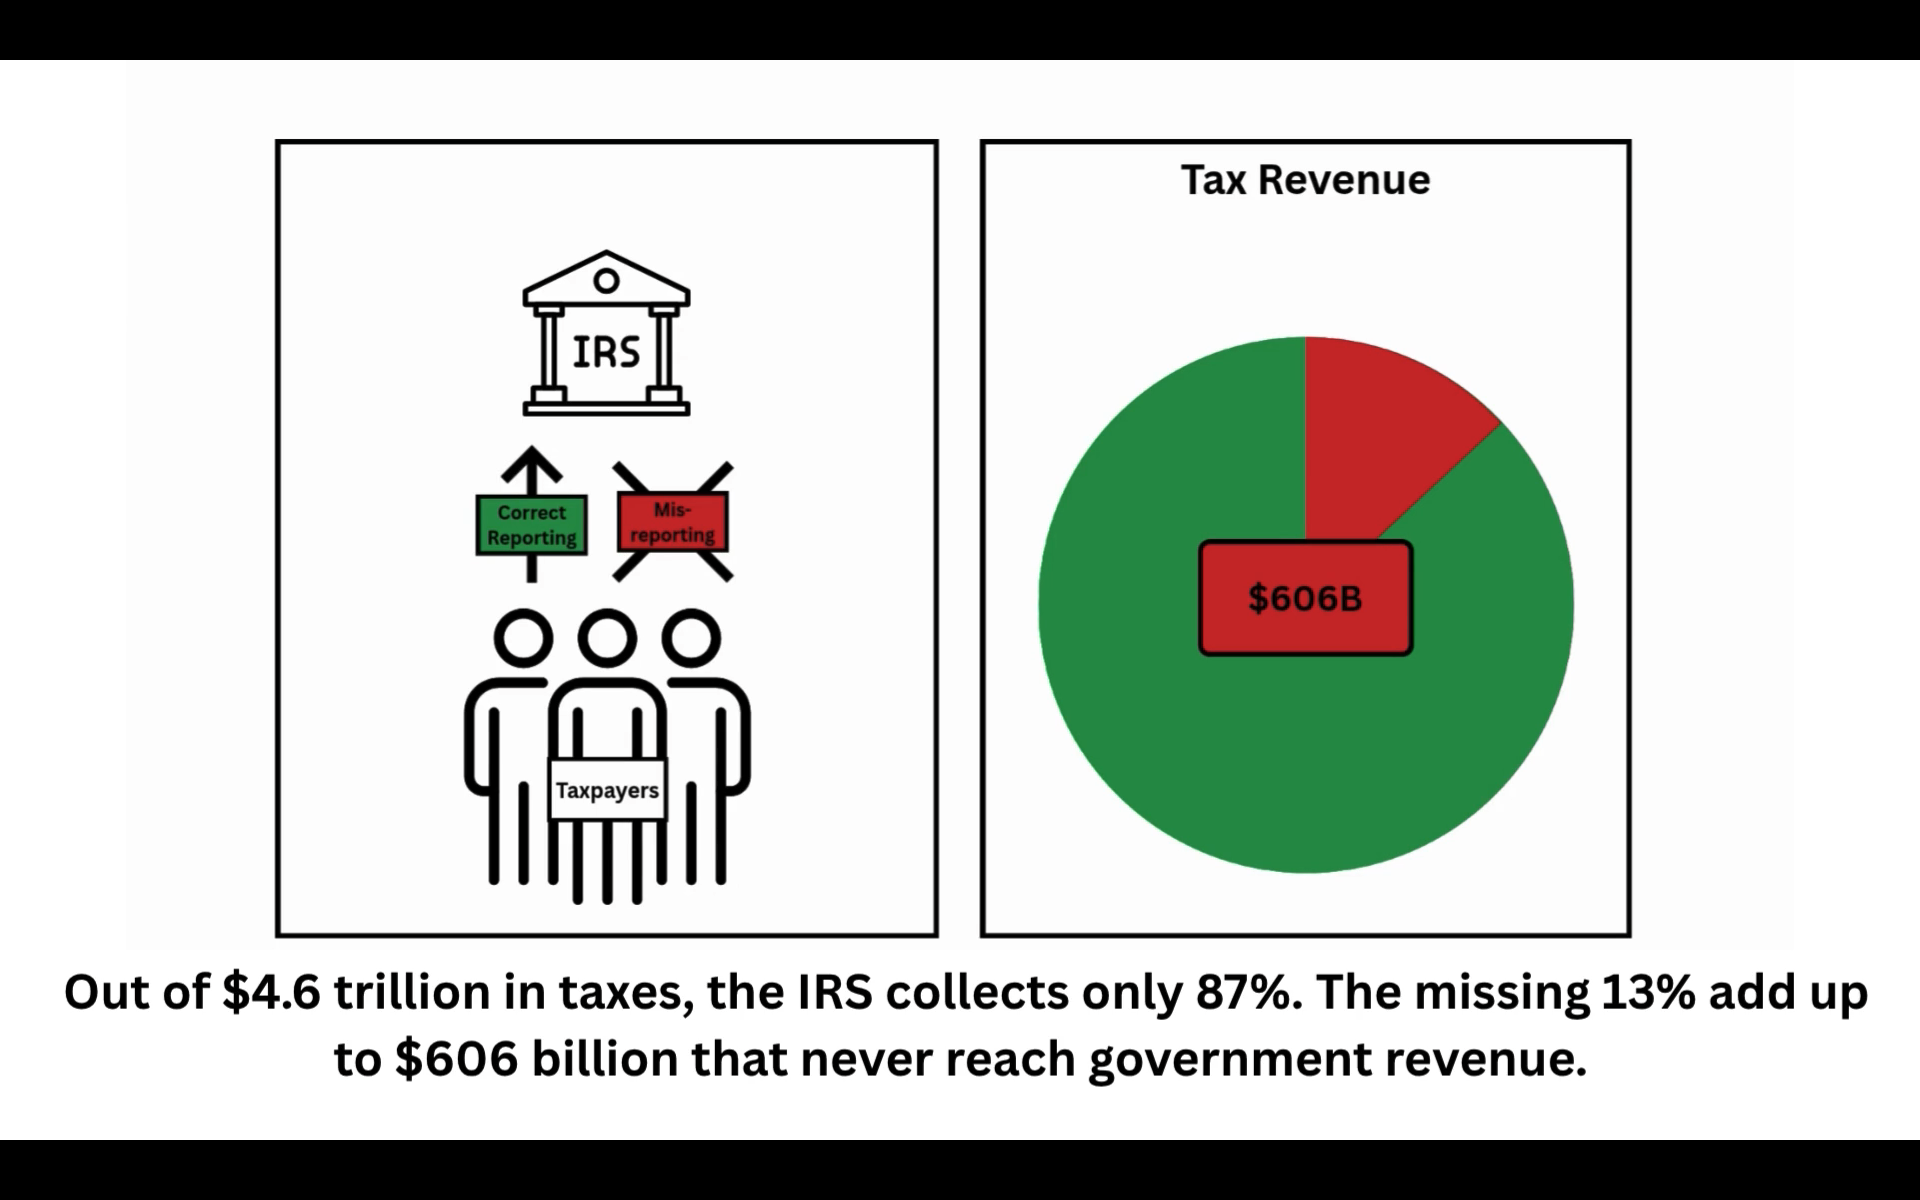
\includegraphics[width=\linewidth, trim={0.5cm 2.5cm 0.5cm 2.5cm}, clip]{Figures_Slides/Revenue_1.png}%
}\\[0.5cm]
    %\vspace*{1cm}
\fbox{%
  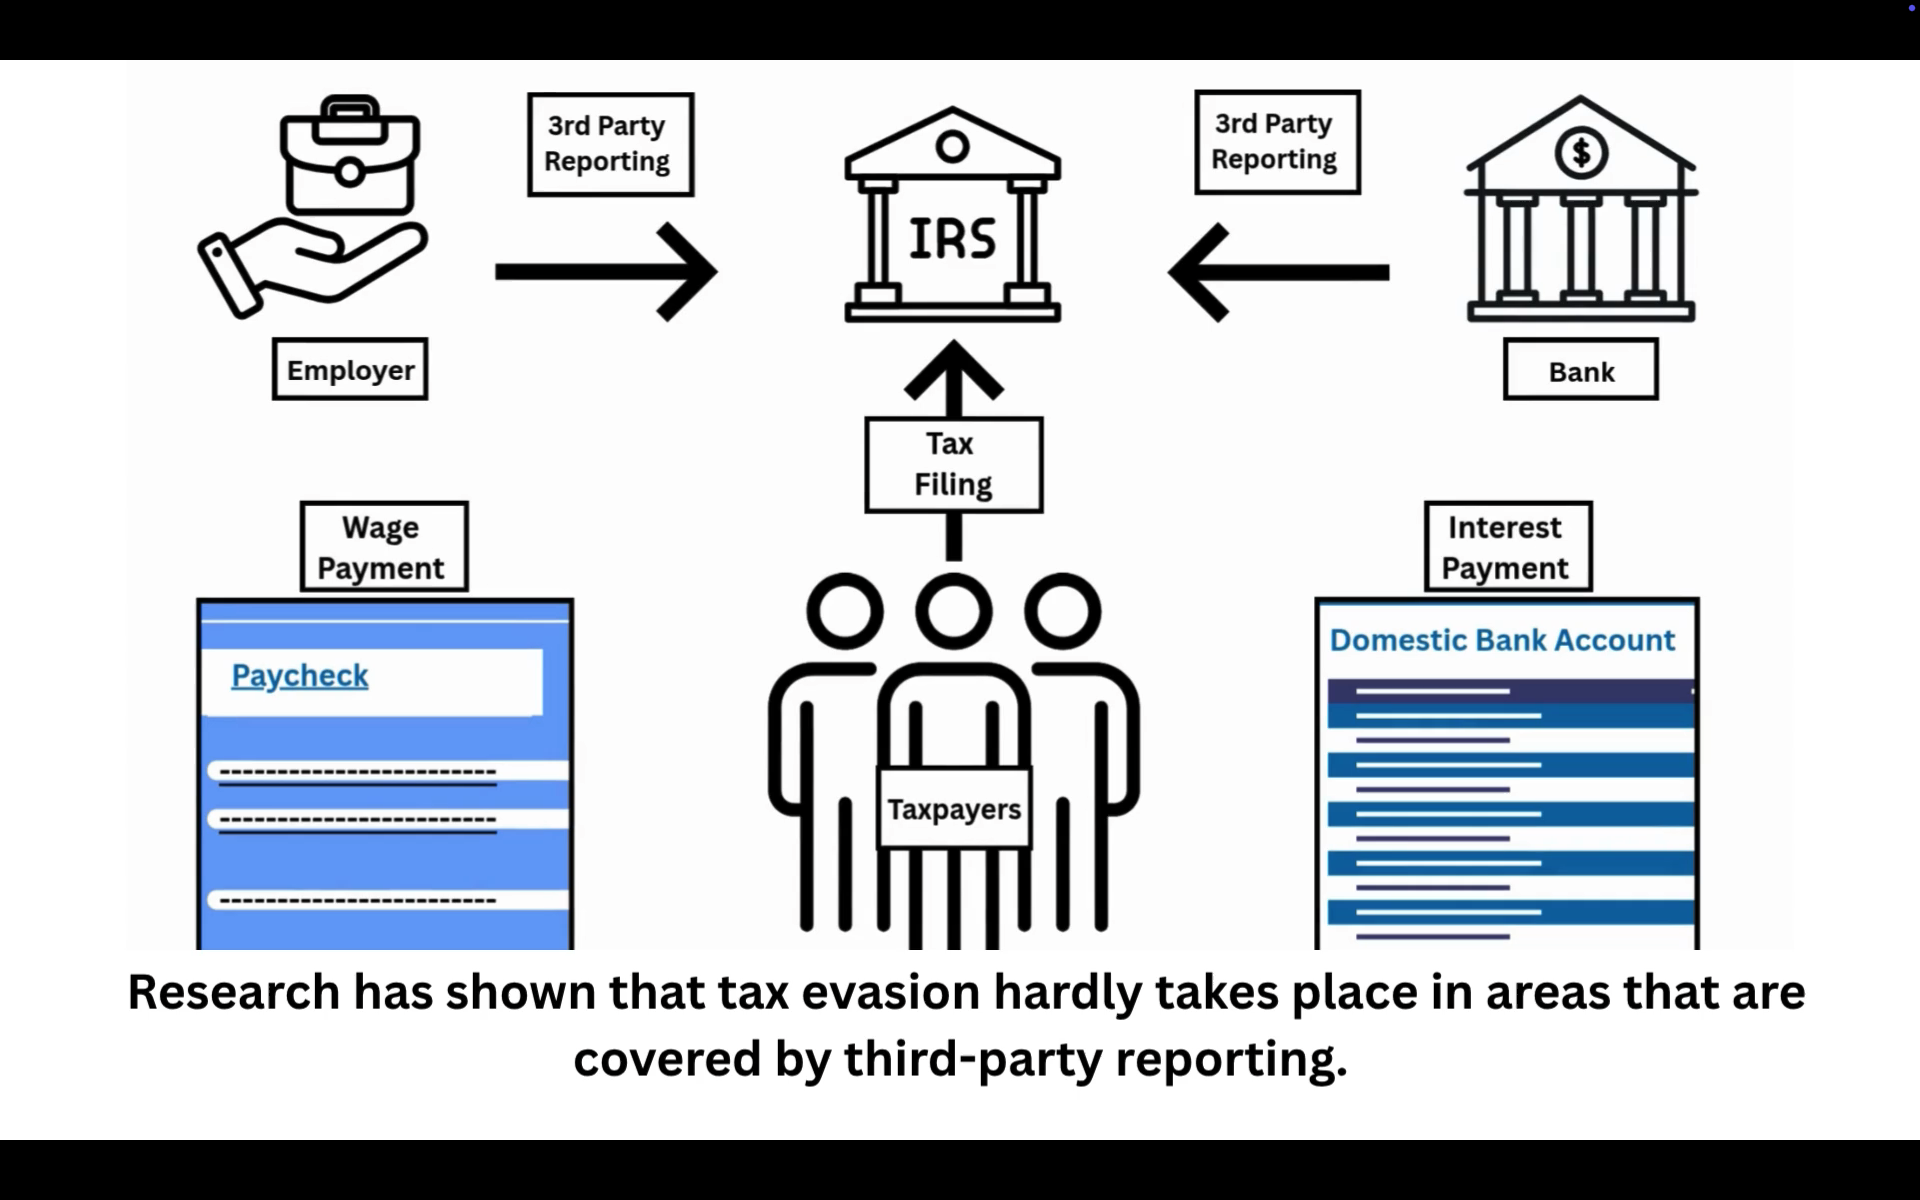
\includegraphics[width=\linewidth, trim={0.5cm 2.5cm 0.5cm 2.5cm}, clip]{Figures_Slides/Revenue_2.png}%
}\\[0.5cm]
\hfill \hyperlink{frame:treatments}{\beamergotobutton{Back}}
  \end{column}
\end{columns}
\end{frame}

\begin{frame}{Evasion: Inequality}
\label{frame:Evasioninequality}
\begin{columns}[T] % align columns at the top
  \begin{column}{0.45\textwidth} % left side for text
    \begin{itemize}
    \item Information about economic problem
    \begin{itemize}
    \vspace{0.25em}
        \item \alert{Extent} of tax evasion\footnote{\cite{IRS_TaxGap_2022_Pub5869}}
        \vspace{0.25em}
        \item \alert{Distribution} of tax evasion\footnote{\cite{guyton2021tax}}
    \end{itemize}
    \vspace{1.5em} 
    \item Information about policy
    \begin{itemize}
        \vspace{0.25em} 
        \item Third-party reporting \& IEoI \alert{reduces tax evasion}\footnote{ \cite{kleven2011unwilling,pomeranz2015no,kleven2016can,slemrod2017does,jensen2022employment,baselgia2023compliance,boas2024taxing}}
        \vspace{2.5em}
    \end{itemize}
    \end{itemize}
  \end{column}
  
  \begin{column}{0.45\textwidth} % right side for image
    %\vspace{0.3cm}
    \centering
    \vspace{-0.5em}
    \fbox{%
  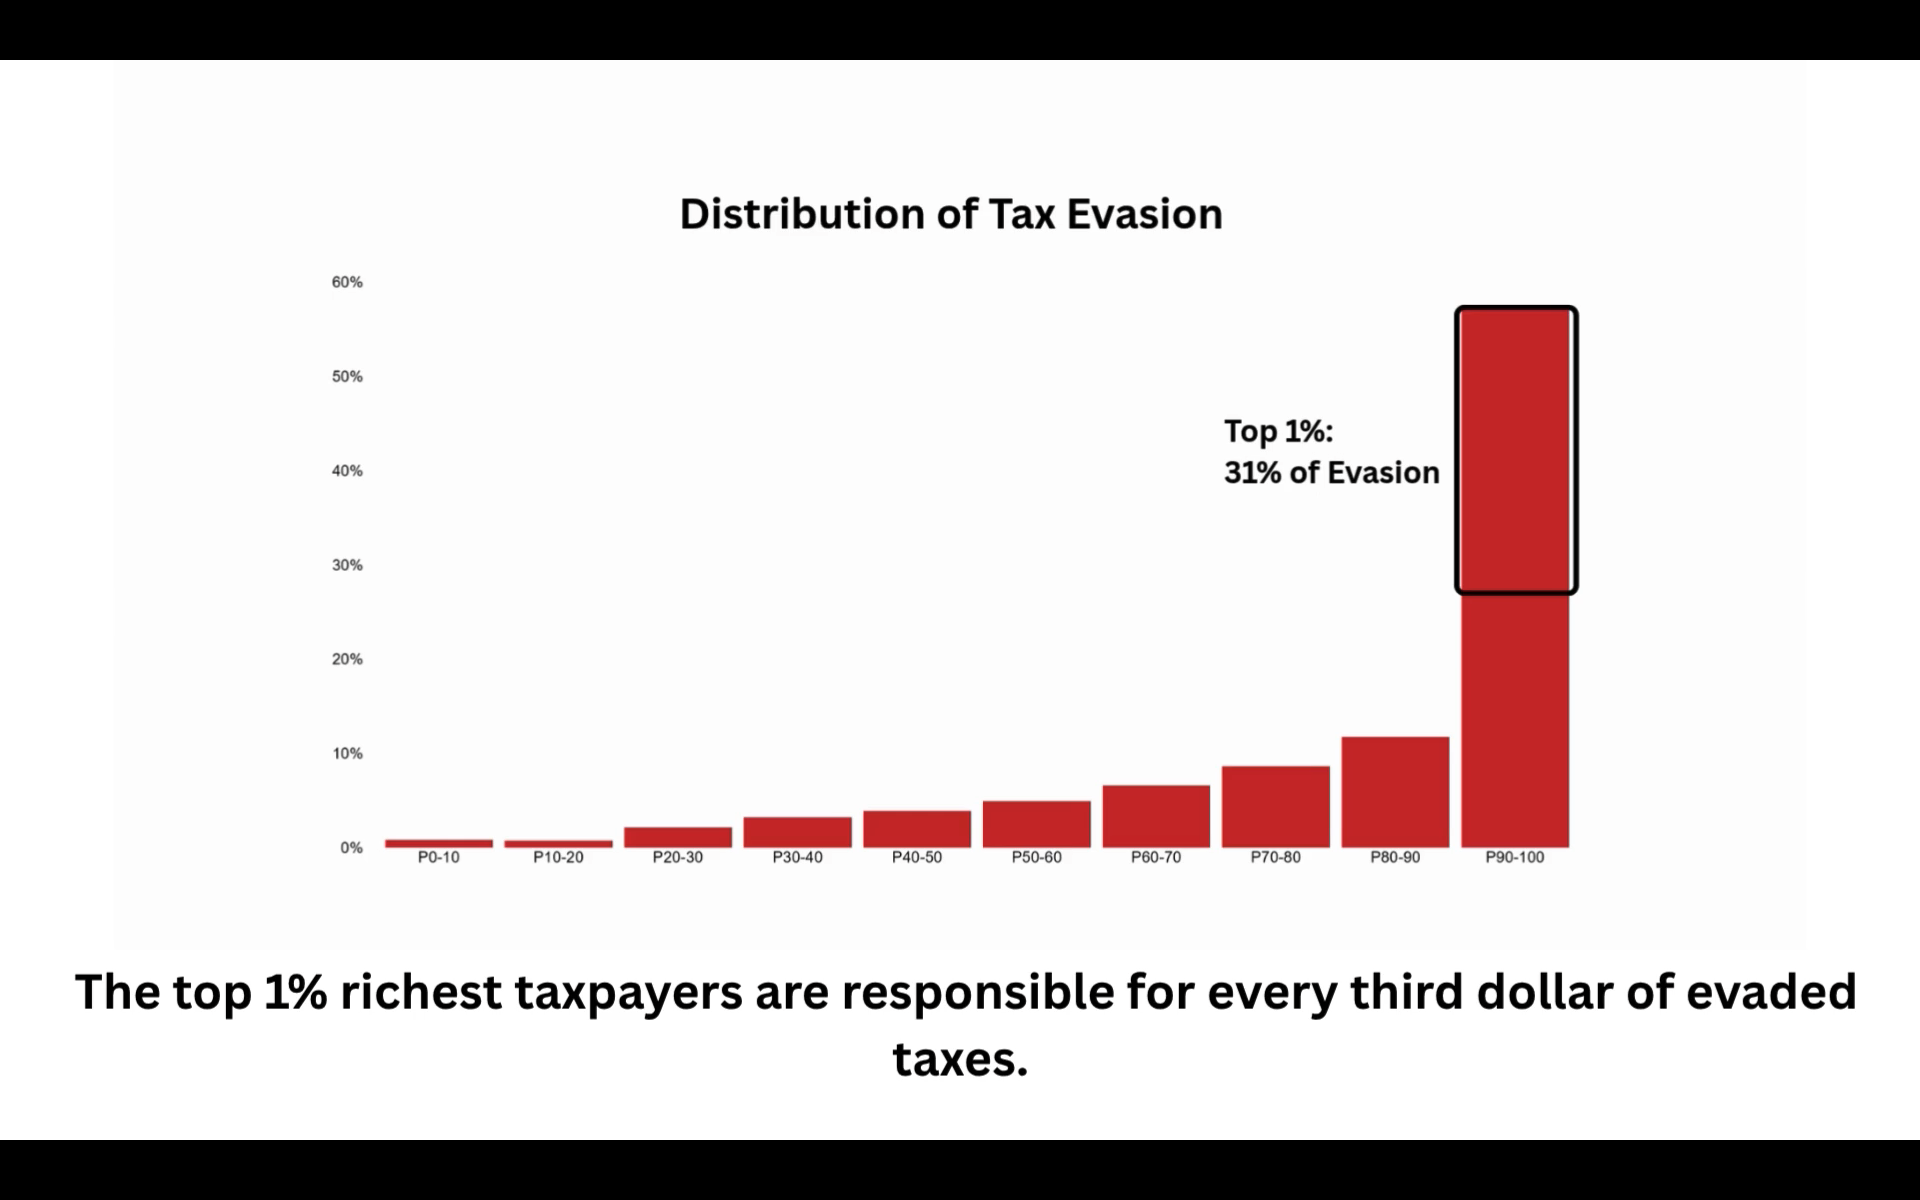
\includegraphics[width=\linewidth, trim={0.5cm 2.5cm 0.5cm 2.5cm}, clip]{Figures_Slides/Inequality_1.png}%
}\\[0.5cm]
    %\vspace*{1cm}
\fbox{%
  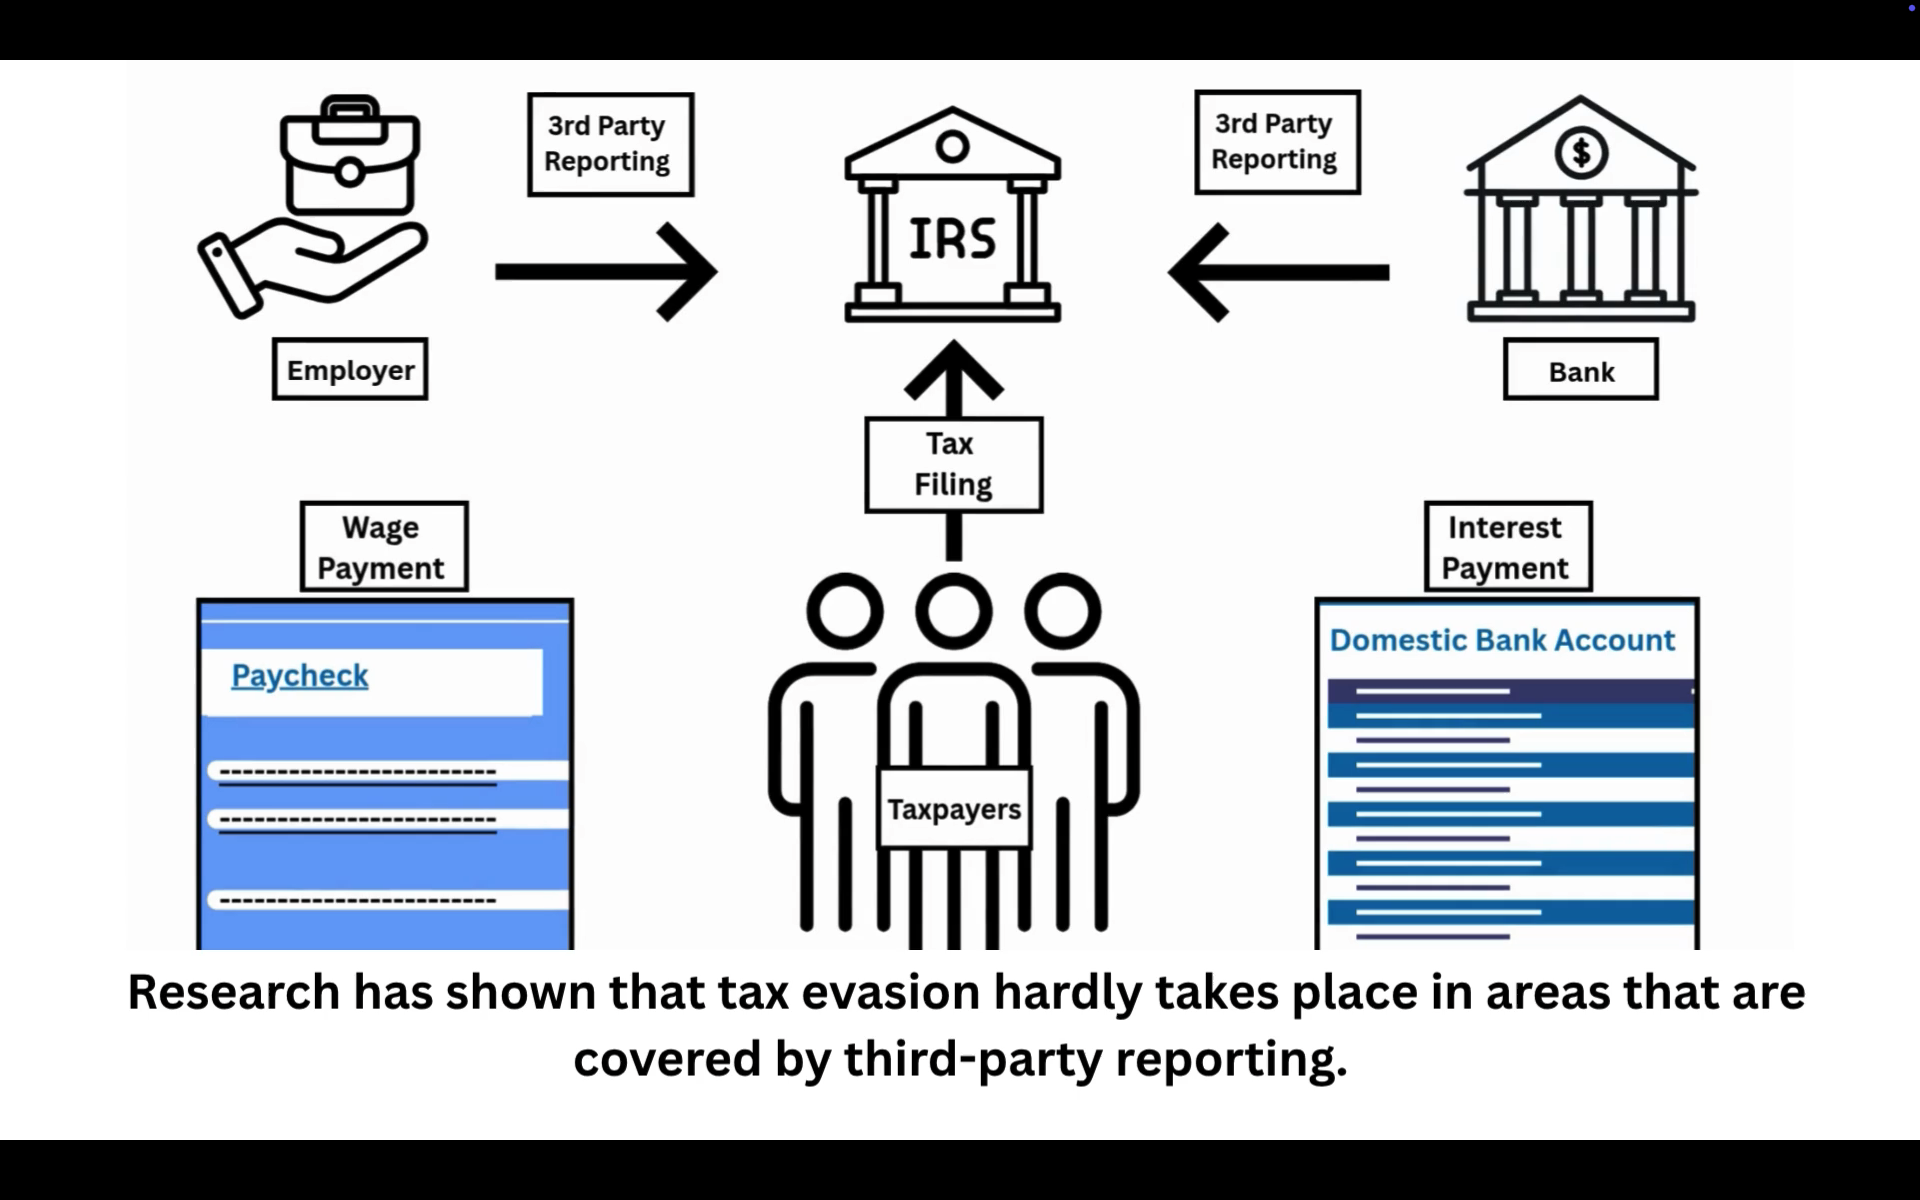
\includegraphics[width=\linewidth, trim={0.5cm 2.5cm 0.5cm 2.5cm}, clip]{Figures_Slides/Revenue_2.png}%
}\\[0.5cm]
\hfill \hyperlink{frame:treatments}{\beamergotobutton{Back}}
  \end{column}
\end{columns}
\end{frame}

\begin{frame}{Filing Costs}
\label{frame:Taxfiling}
\begin{columns}[T] % align columns at the top
  \begin{column}{0.45\textwidth} % left side for text
    \begin{itemize}
    \item Information about economic problem
    \begin{itemize}
        \vspace{0.25em} 
        \item \alert{Tax filing costs}\footnote{\cite{IRS2022}}
    \end{itemize}
    \vspace{2.5em} 
    \item Information about policy
    \begin{itemize}
        \vspace{0.25em} 
        \item Tax software and prepopulated tax returns \alert{reduce tax filing costs}.
        \vspace{0.25em} 
        \item Third-party reporting is \alert{important for prepopulated returns}.\footnote{\cite{goodman2023automated}}
        \vspace{1em}
    \end{itemize}
    \end{itemize}
  \end{column}
  
  \begin{column}{0.45\textwidth} % right side for image
    %\vspace{0.3cm}
    \centering
    \vspace{-0.5em}
    \fbox{%
  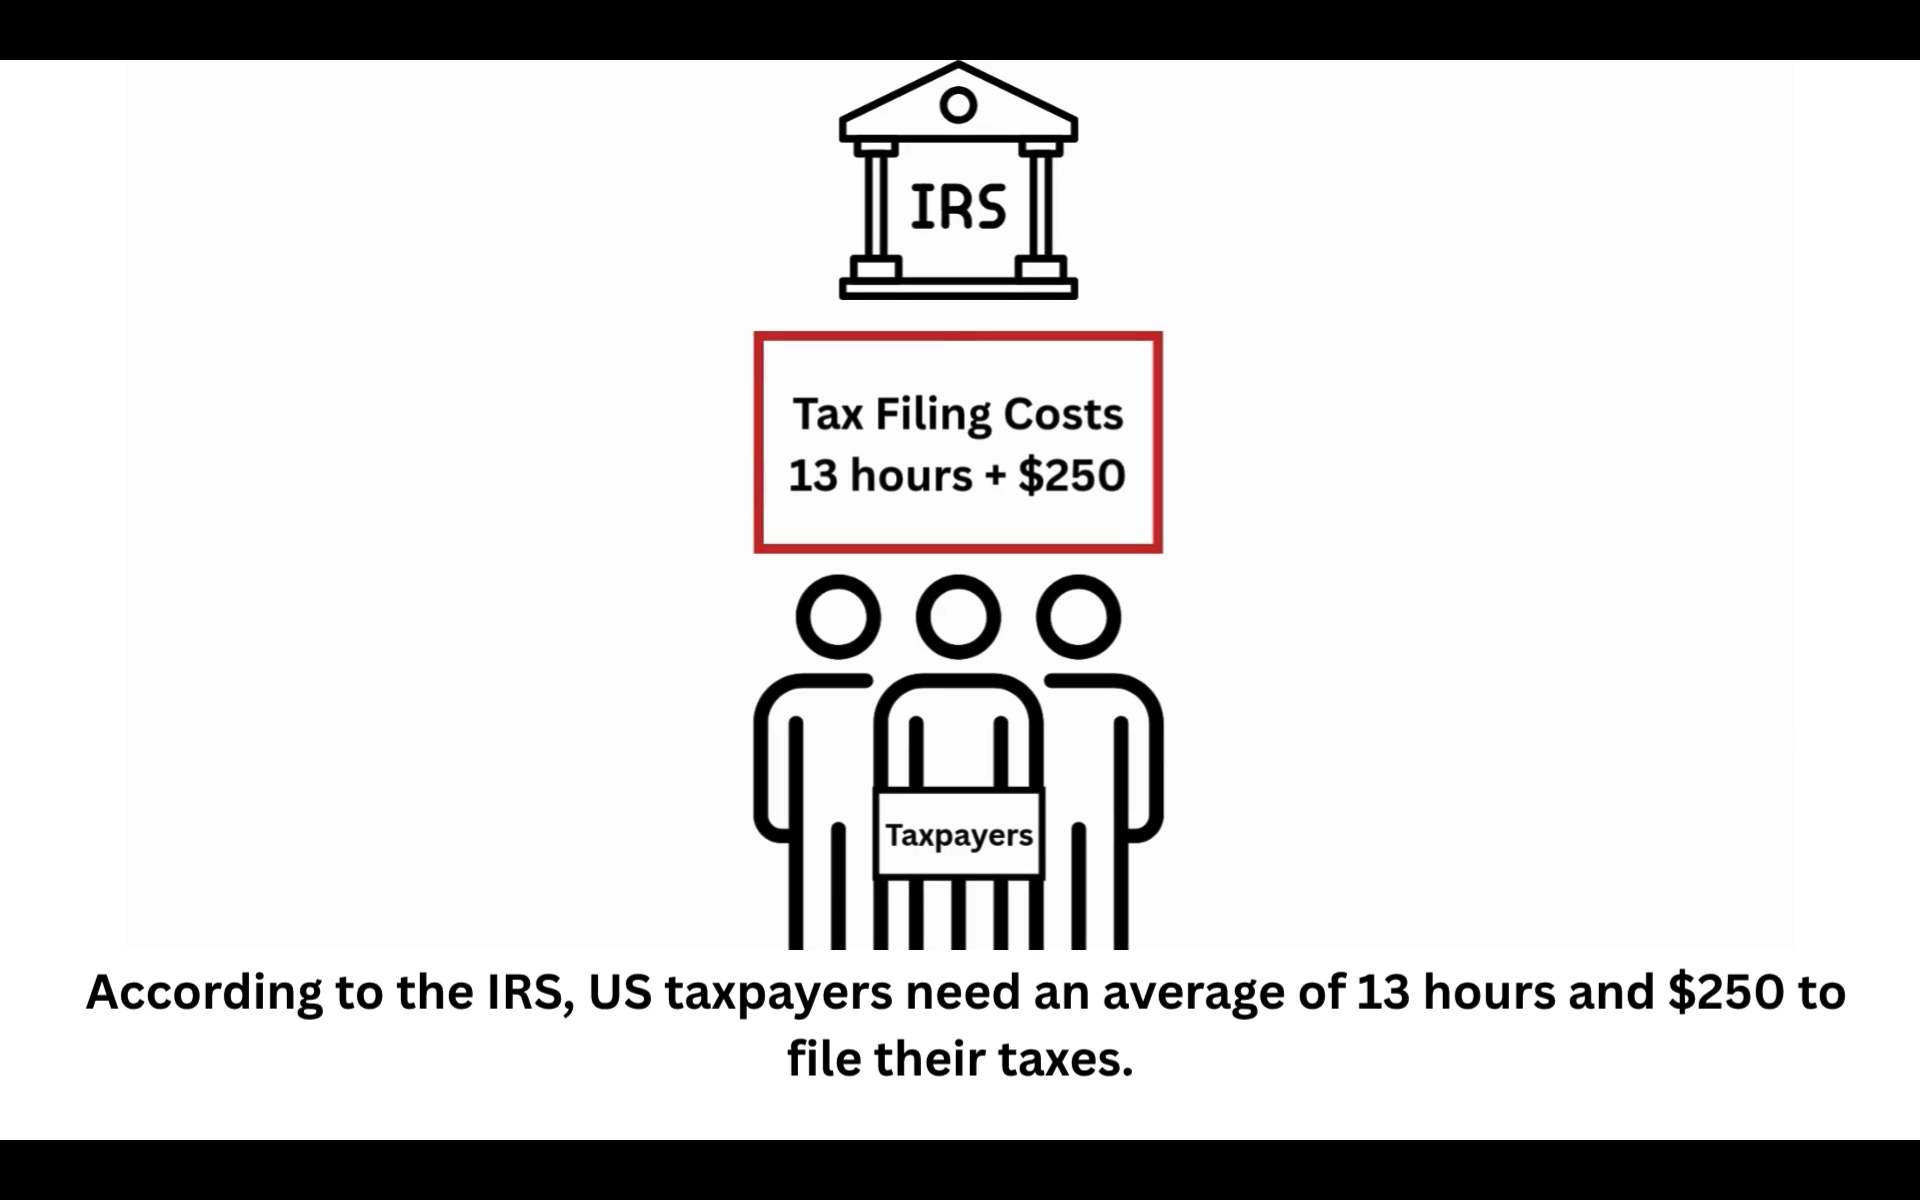
\includegraphics[width=\linewidth, trim={0.5cm 2.5cm 0.5cm 2.5cm}, clip]{Figures_Slides/Filing_3.png}%
}\\[0.5cm]
    %\vspace*{1cm}
\fbox{%
  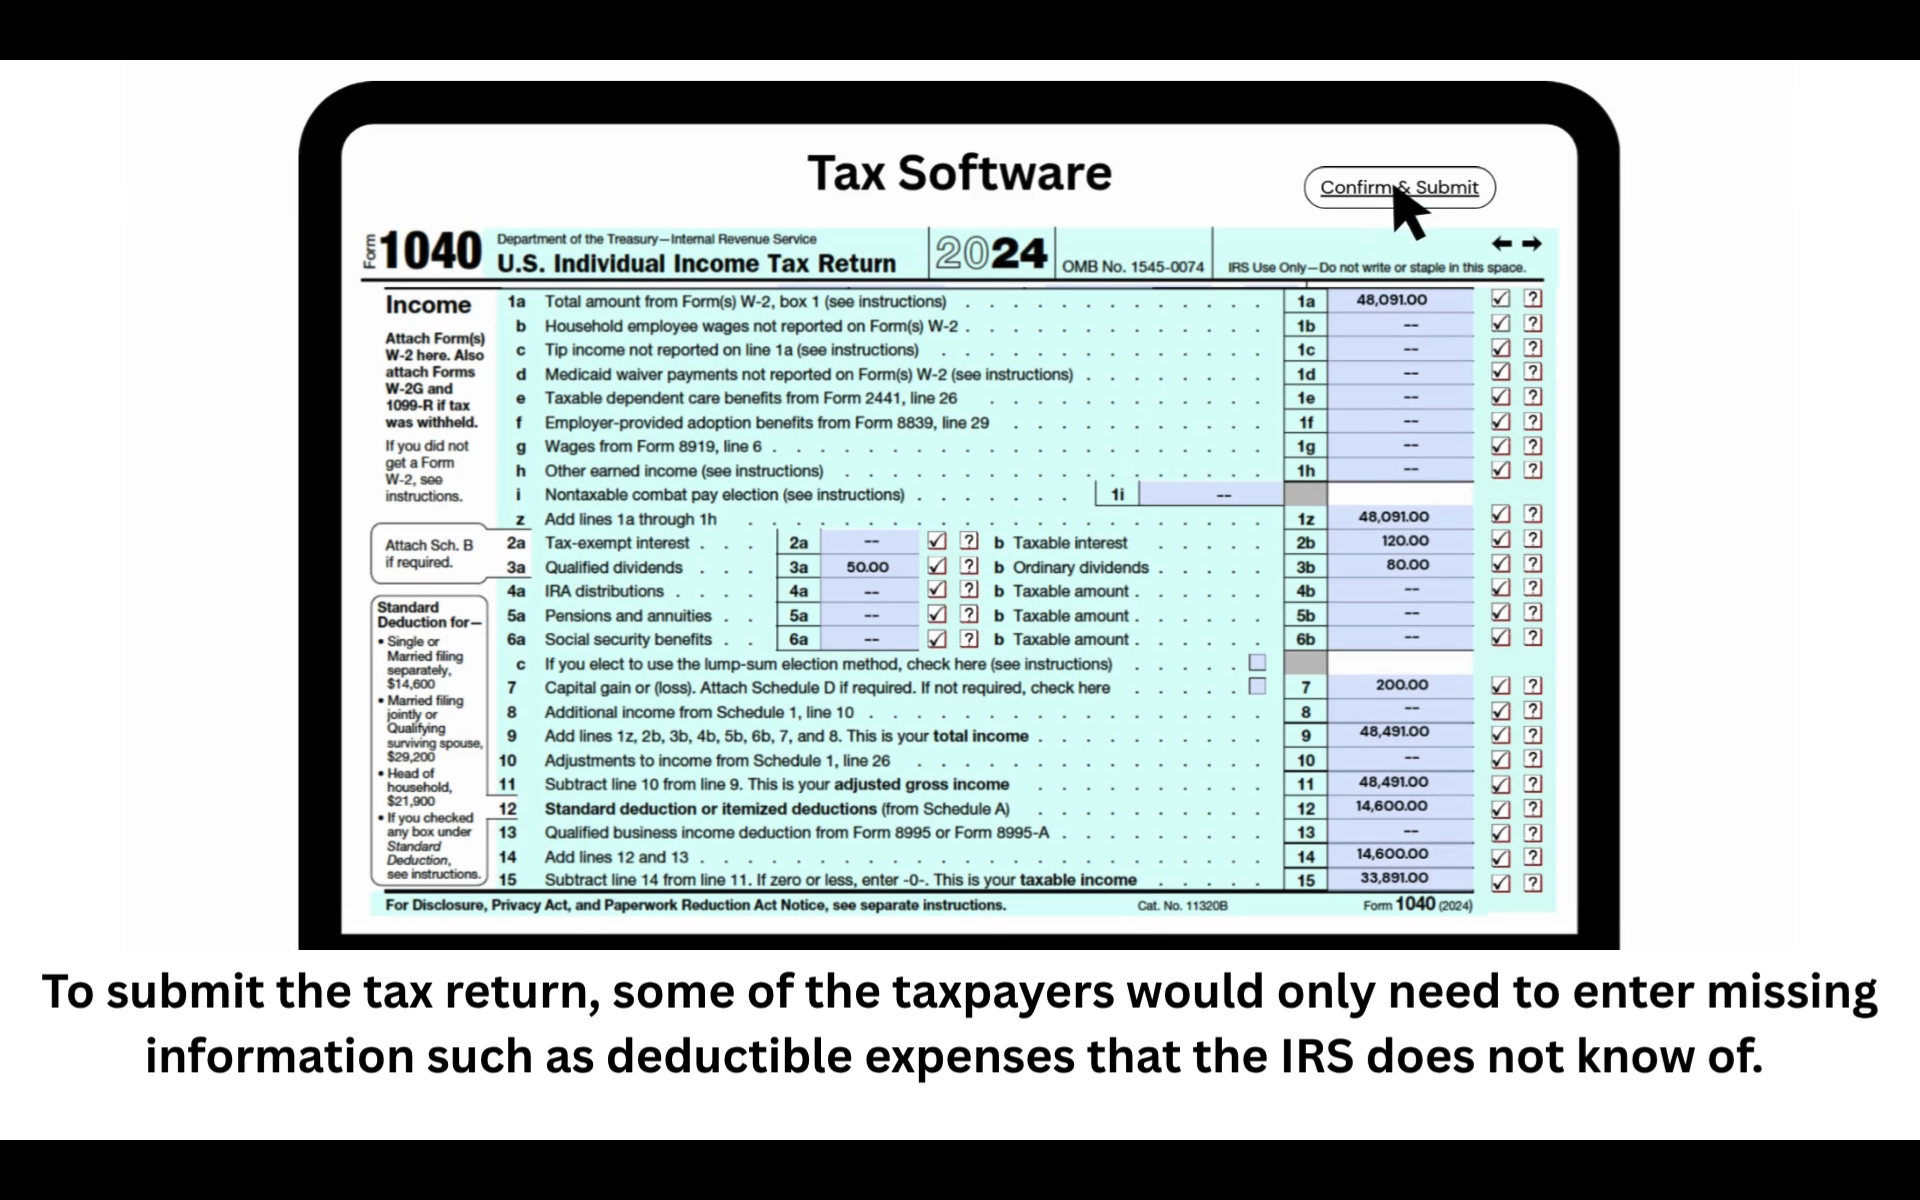
\includegraphics[width=\linewidth, trim={0.5cm 2.5cm 0.5cm 2.5cm}, clip]{Figures_Slides/Filing_1.png}%
}\\[0.5cm]
\hfill \hyperlink{frame:treatments}{\beamergotobutton{Back}}
  \end{column}
\end{columns}
\end{frame}

\begin{frame}{Full Info}
\label{frame:Fullinfo}
\begin{columns}[T] % align columns at the top
  \begin{column}{0.35\textwidth} % right side for image
    %\vspace{0.3cm}
    \centering
    Filing Treatment
    \vspace{-0.5em}
    \fbox{%
  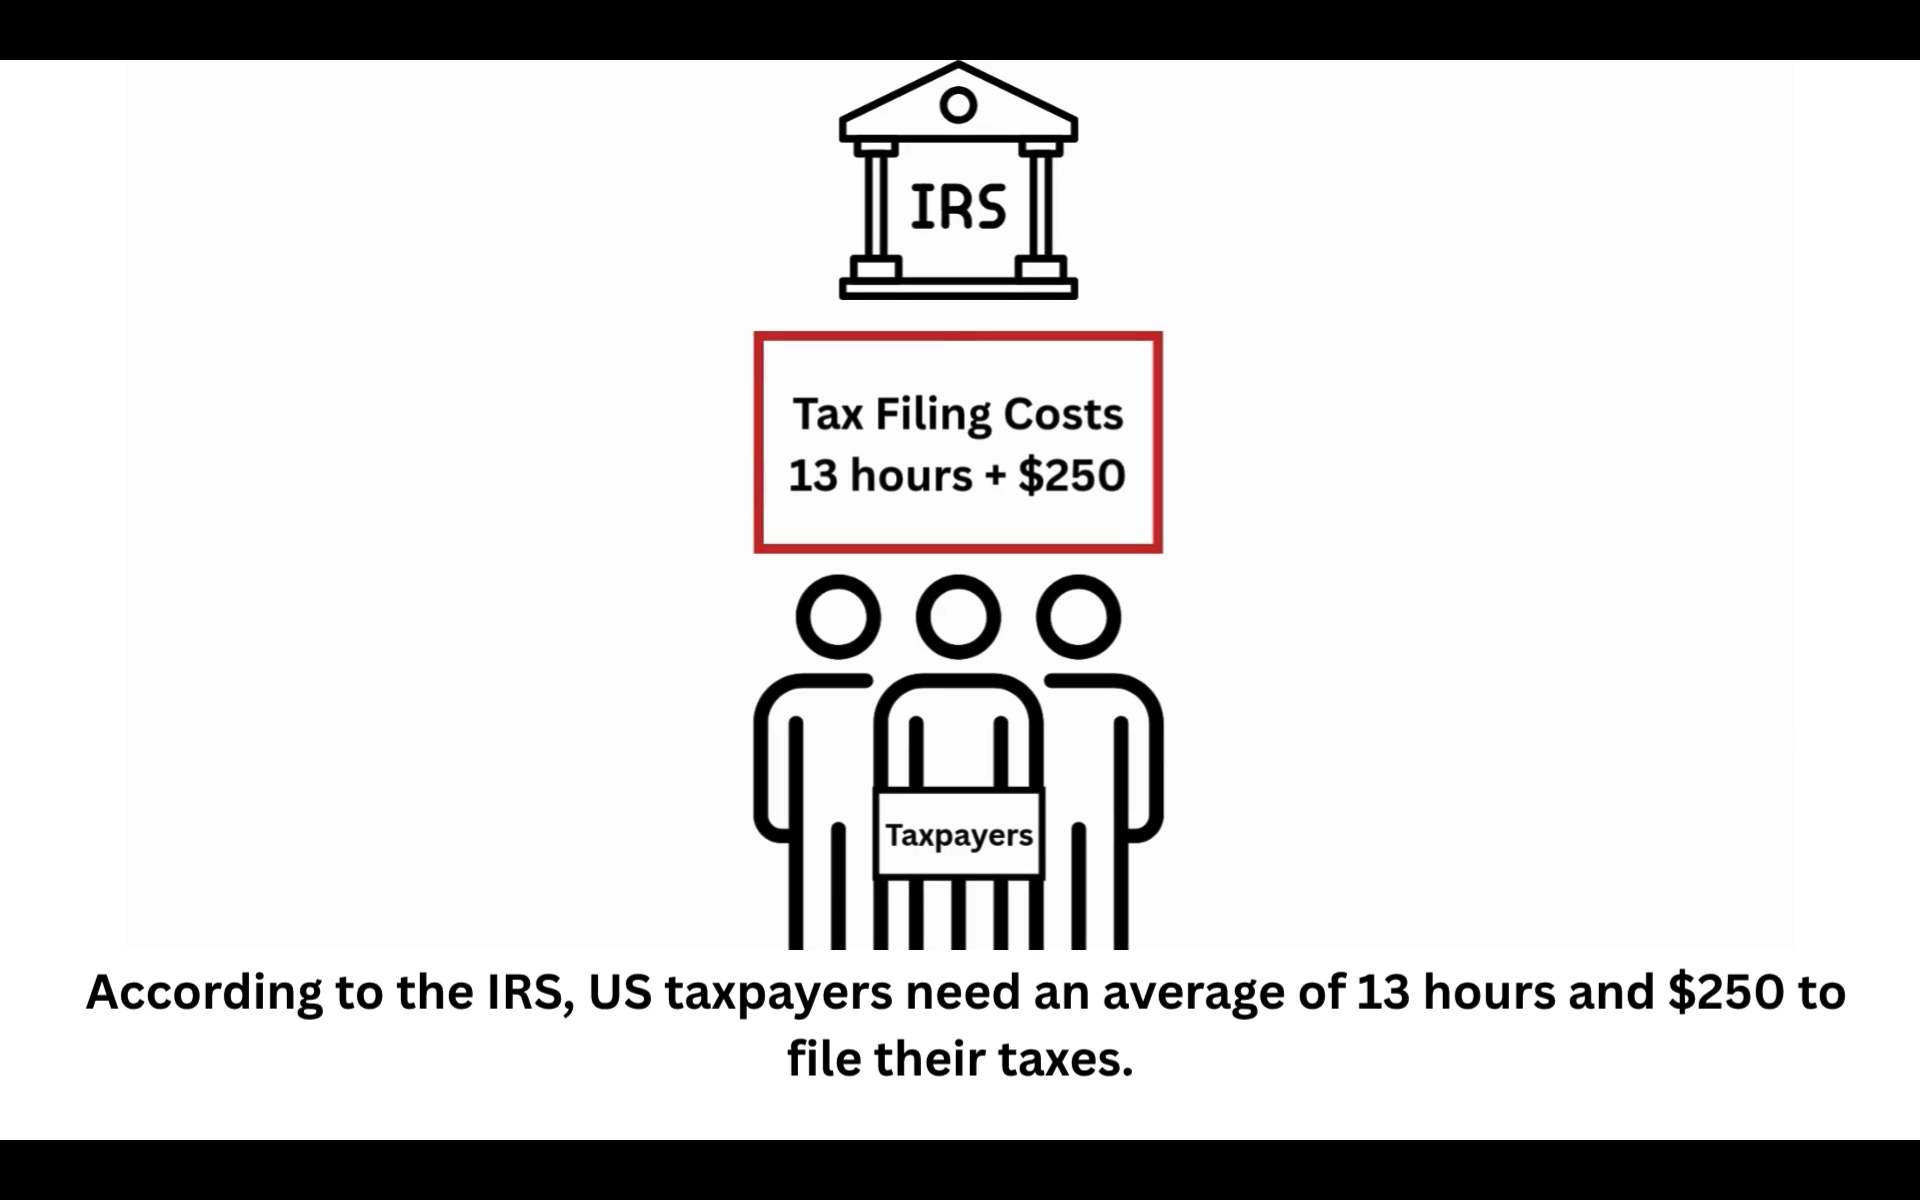
\includegraphics[width=\linewidth, trim={0.5cm 2.5cm 0.5cm 2.5cm}, clip]{Figures_Slides/Filing_3.png}%
}\\[0.5cm]
    %\vspace*{1cm}
\fbox{%
  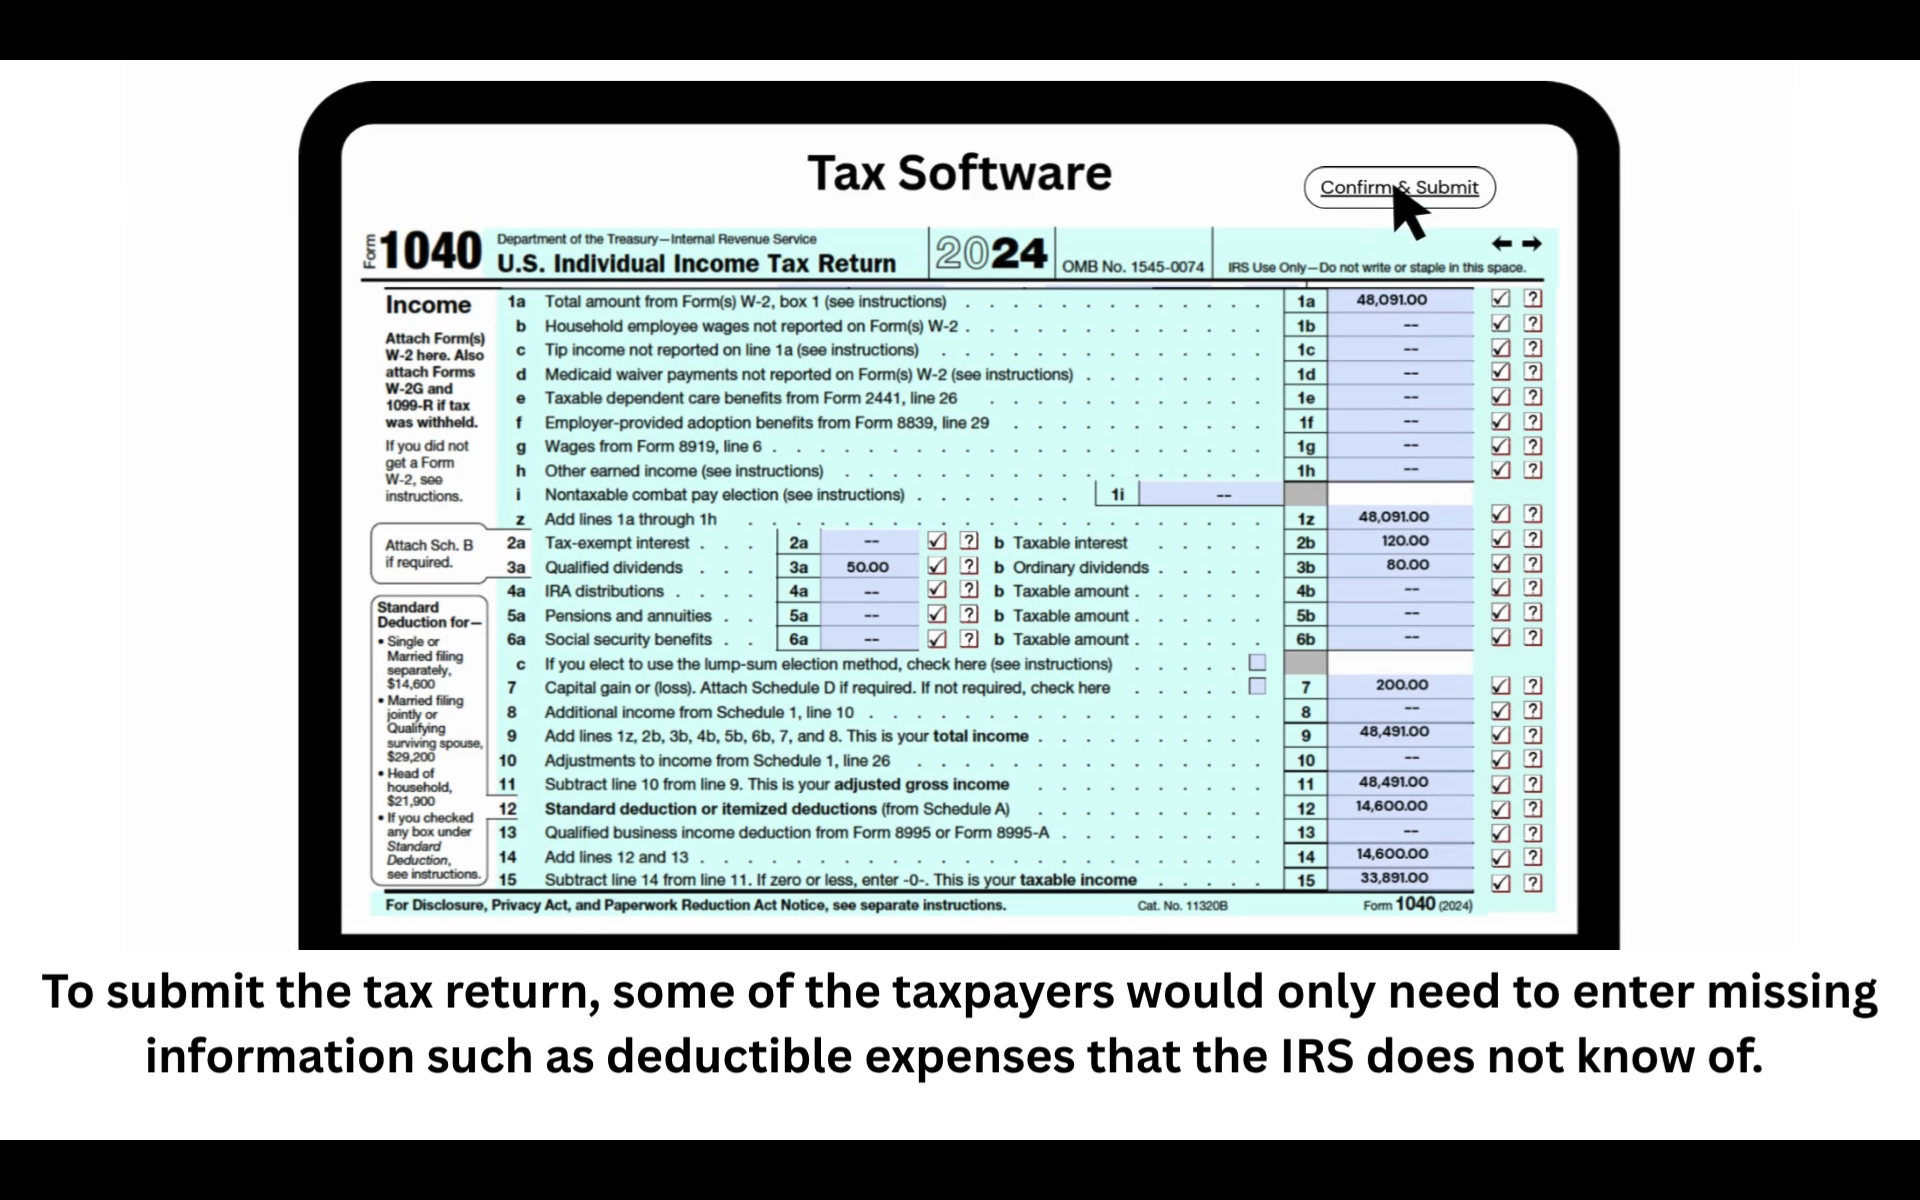
\includegraphics[width=\linewidth, trim={0.5cm 2.5cm 0.5cm 2.5cm}, clip]{Figures_Slides/Filing_1.png}%
}
  \end{column}
  \begin{column}{0.05\textwidth}
  \centering
  \vspace{2cm}
  \Large $\longrightarrow$
\\[0.5cm]
\Large $\longrightarrow$
\\[0.5cm]
\Large $\longrightarrow$
  \end{column}
  \begin{column}{0.35\textwidth} % left side for text
    %\vspace{0.3cm}
    \centering
      Inequality Treatment
    \vspace{-0.5em}
    \fbox{%
  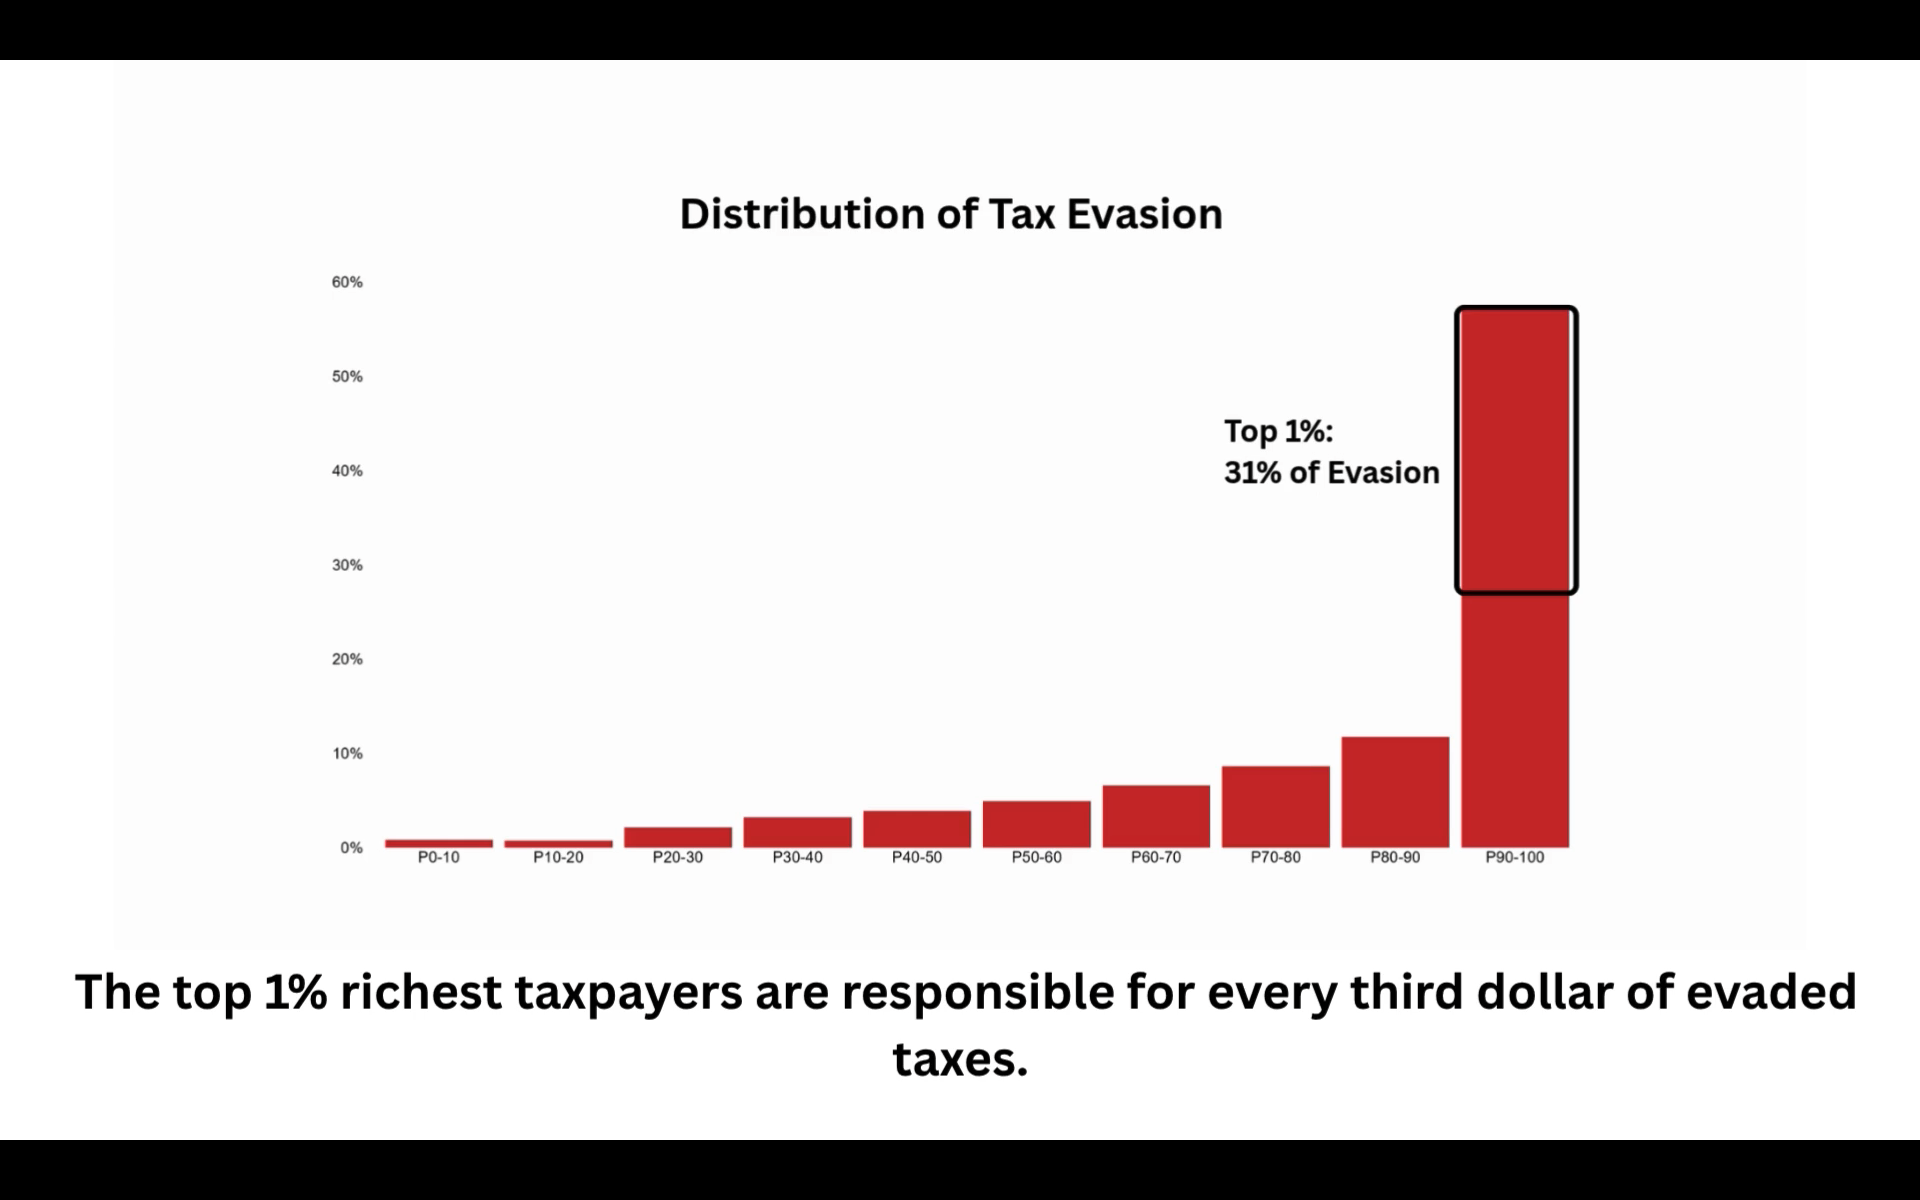
\includegraphics[width=\linewidth, trim={0.5cm 2.5cm 0.5cm 2.5cm}, clip]{Figures_Slides/Inequality_1.png}%
}\\[0.5cm]
    %\vspace*{1cm}
\fbox{%
  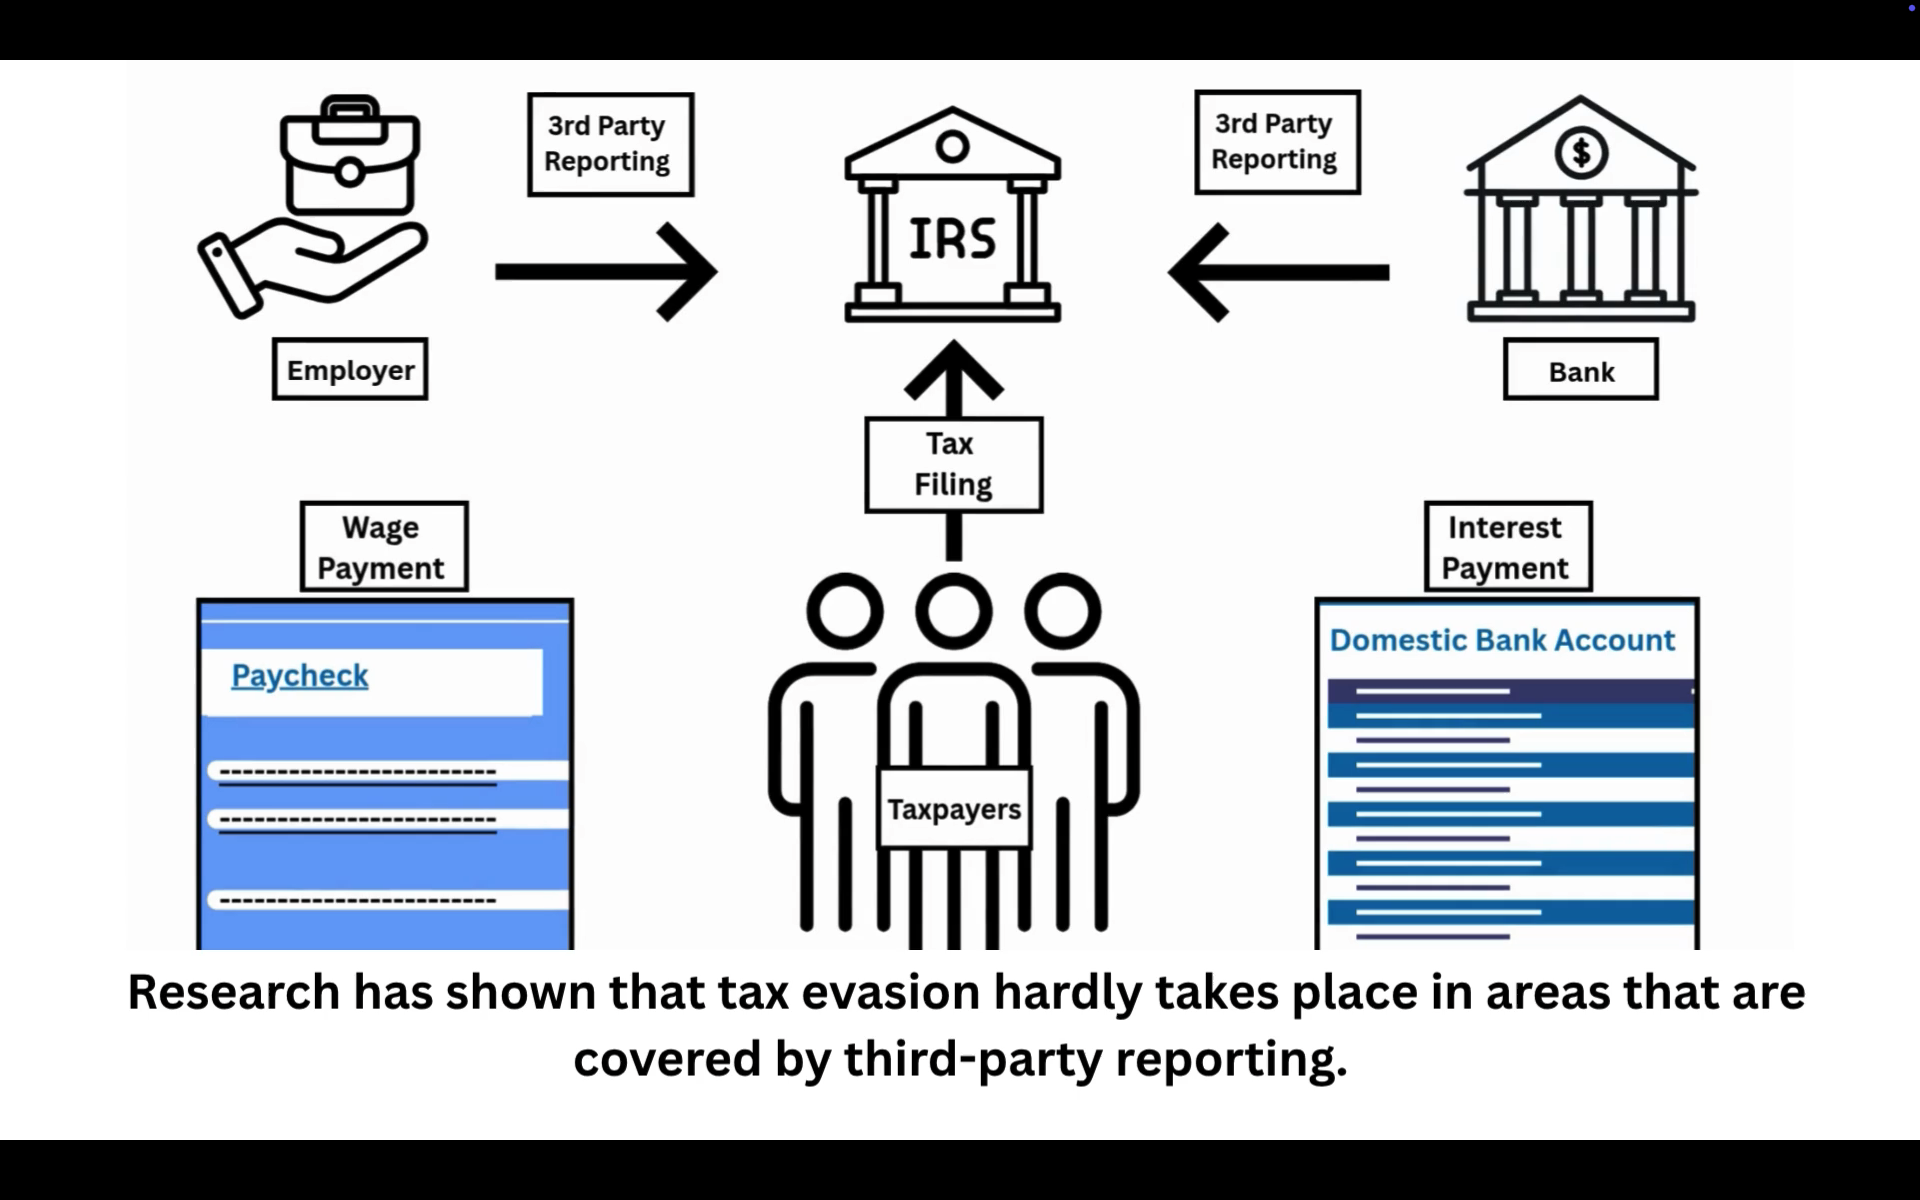
\includegraphics[width=\linewidth, trim={0.5cm 2.5cm 0.5cm 2.5cm}, clip]{Figures_Slides/Revenue_2.png}%
}
  \end{column}

\end{columns}
\vspace{0.3cm}
\centering

\hfill \hyperlink{frame:treatments}{\beamergotobutton{Back}}
\end{frame}


%\begin{frame}[label=Prior_Perceptions]{Perceptions about Underlying \\ Factors}
%\begin{columns}[T] % align columns at the top
%  \begin{column}{0.45\textwidth} % left side for text
%    \begin{itemize}
%    \item Perception about the tax gap
%    \vspace{0.5em} 
%    \item Perception about tax filing cost
%    \begin{itemize}
%        \item time
%        \item monetary cost
%    \end{itemize}
%    \vspace{2em} 
%    \item[$\Rightarrow$] Understand whether respondents update perceptions. 
%    \end{itemize}
%  \end{column}
%  
%  \begin{column}{0.45\textwidth} % right side for image
%    \centering
%     \vspace{-4em}
%    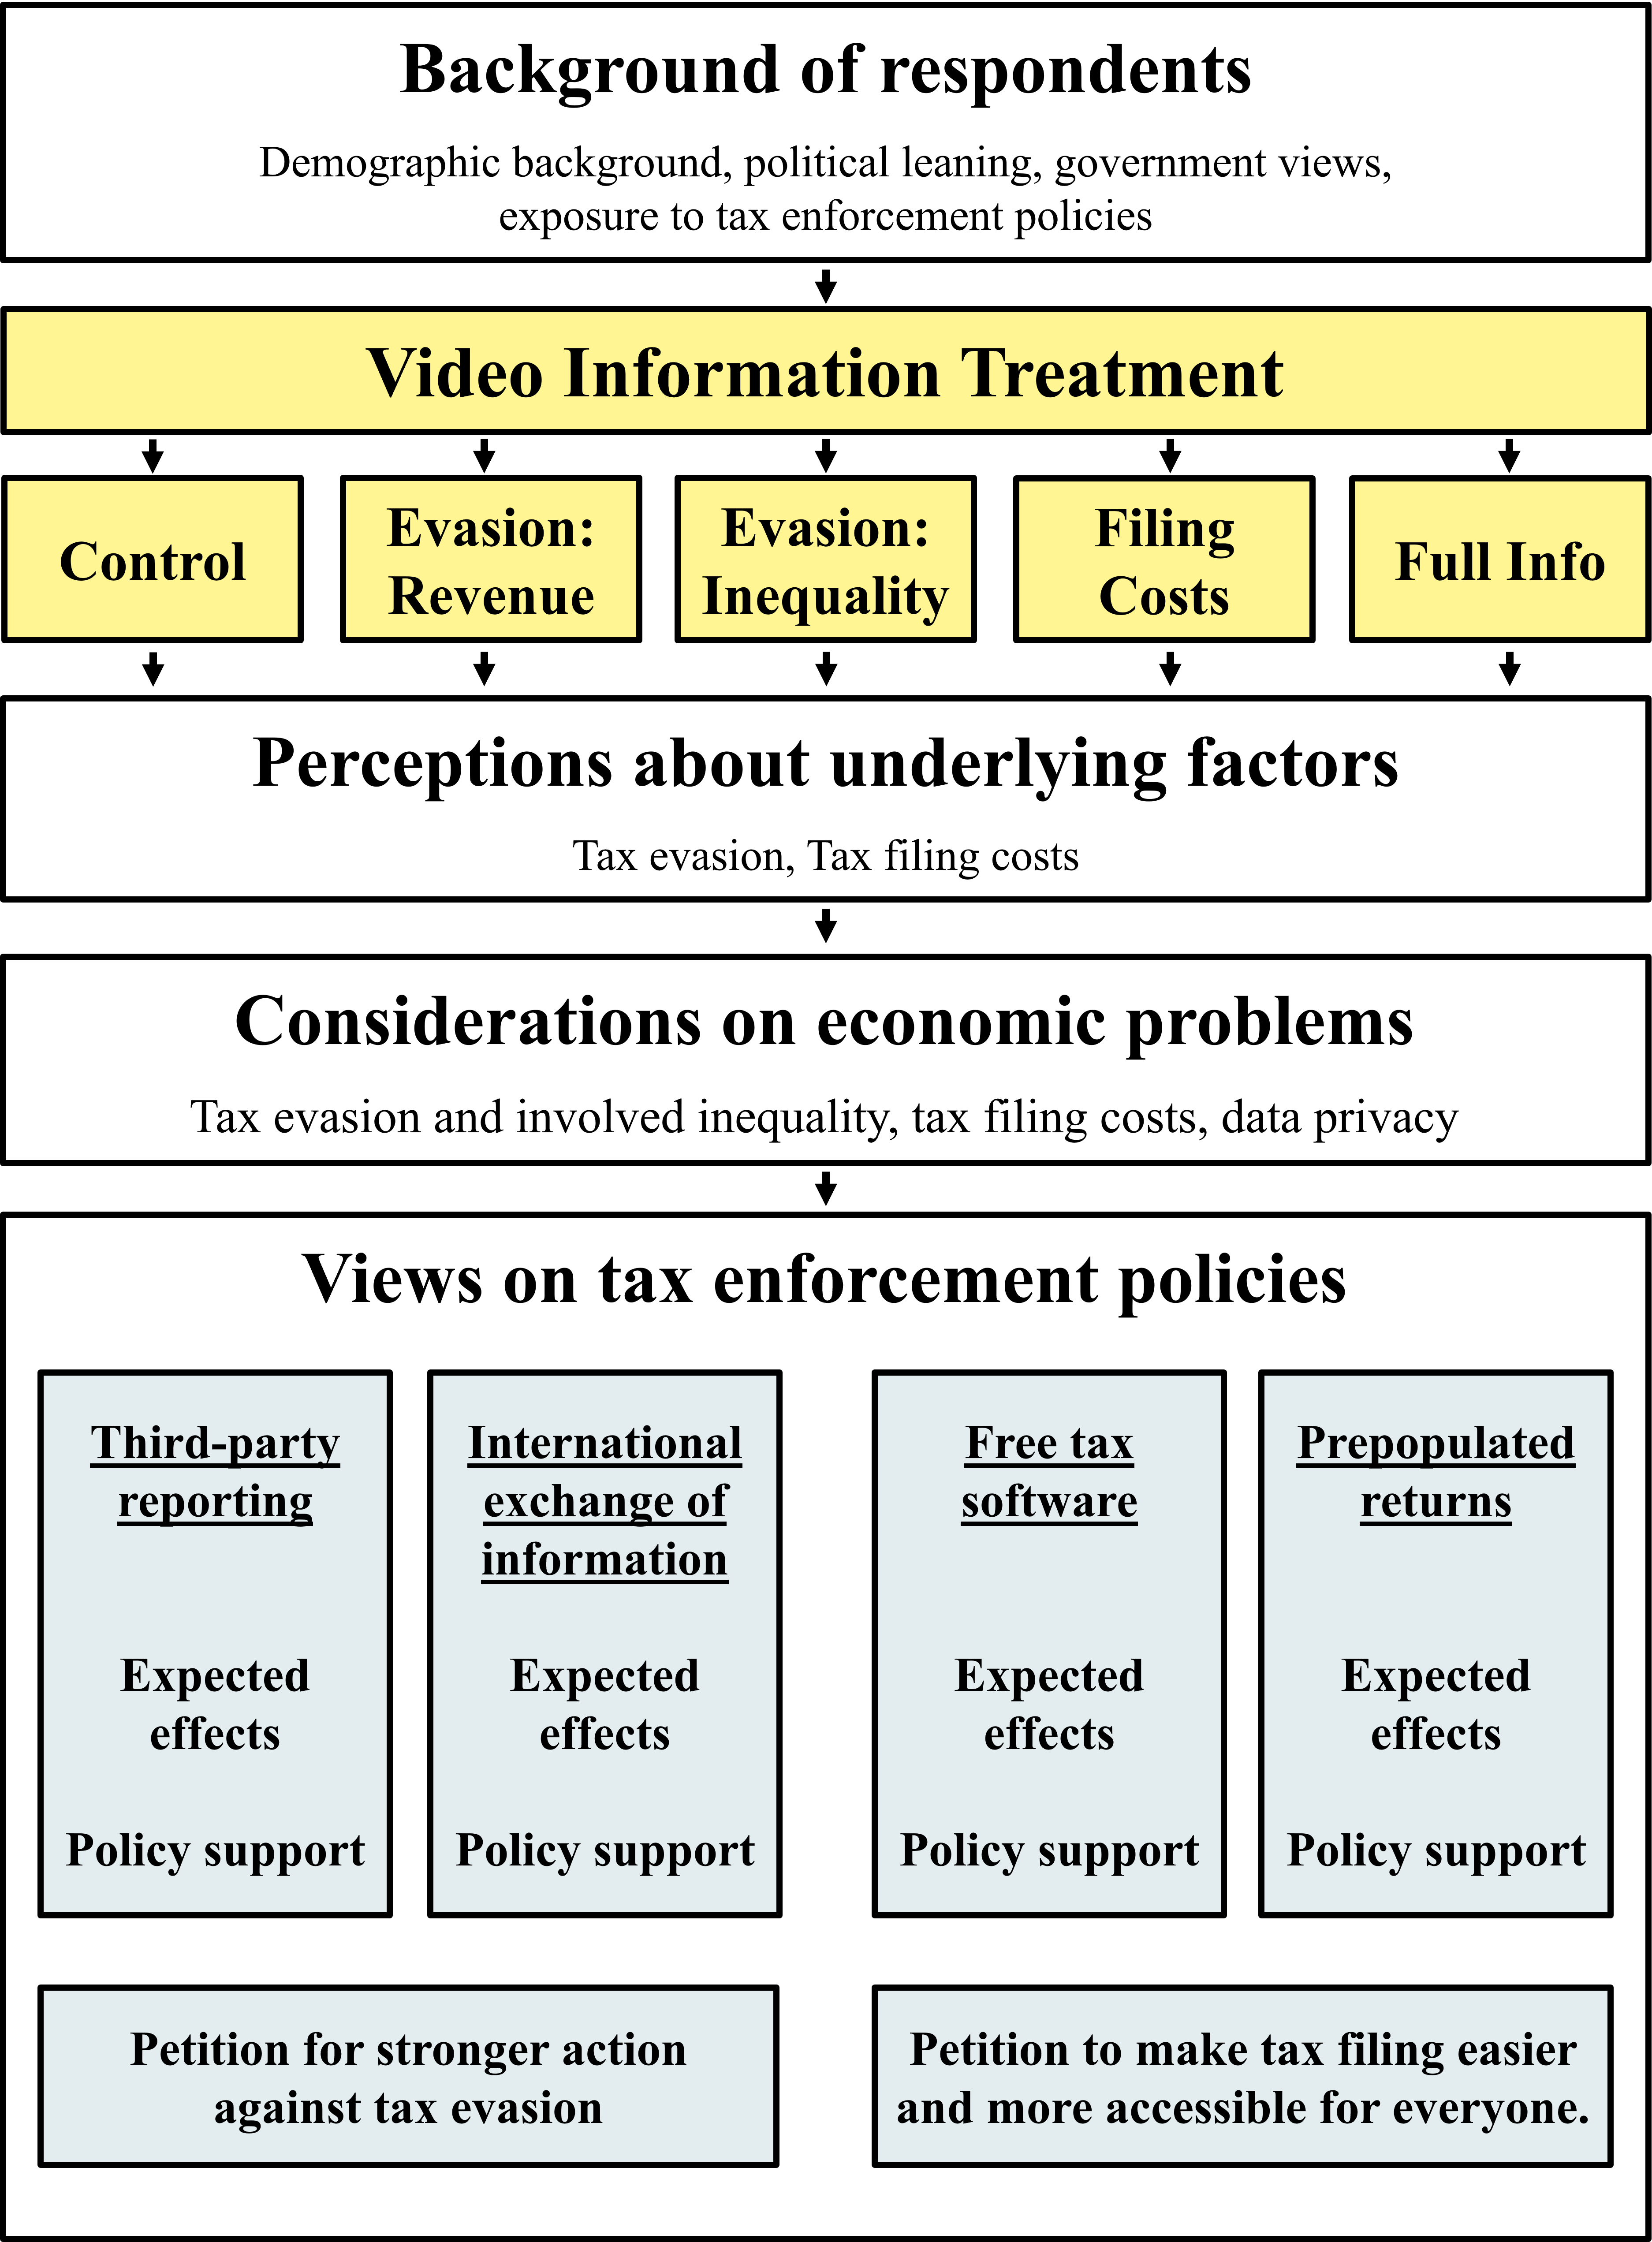
\includegraphics[width=1.05\linewidth]{Figures_Slides/Survey_Overview_Treatments.png}
%  \end{column}
%\end{columns}
%\end{frame}

%\begin{frame}[label=General_Considerations]{General Considerations \hyperlink{General_Considerations_Appendix}{\beamergotobutton{A: GC}}}
%\begin{columns}[T] % align columns at the top
%  \begin{column}{0.45\textwidth} % left side for text
%    \begin{itemize}
%    \item Tax system 
%    \begin{itemize}
%        \item Is it fair? 
%    \end{itemize}
%    \vspace{0.2em} 
%    \item Tax evasion
%    \begin{itemize}
%        \item Is it concerning? 
%        \item Is it important for the government to reduce it?
%    \end{itemize}
%    \vspace{0.2em} 
%    \item Tax filing costs
%    \begin{itemize}
%        \item Are they concerning? 
%        \item Is it important for the government to reduce them?
%    \end{itemize}
%    \vspace{0.2em} 
%    \item Data privacy
%    \begin{itemize}
%        \item Is it a problem if the government collects data on citizens?
%    \end{itemize}
%    \end{itemize}
%  \end{column}
%  
%  \begin{column}{0.45\textwidth} % right side for image
%    \centering
%     \vspace{-2em}     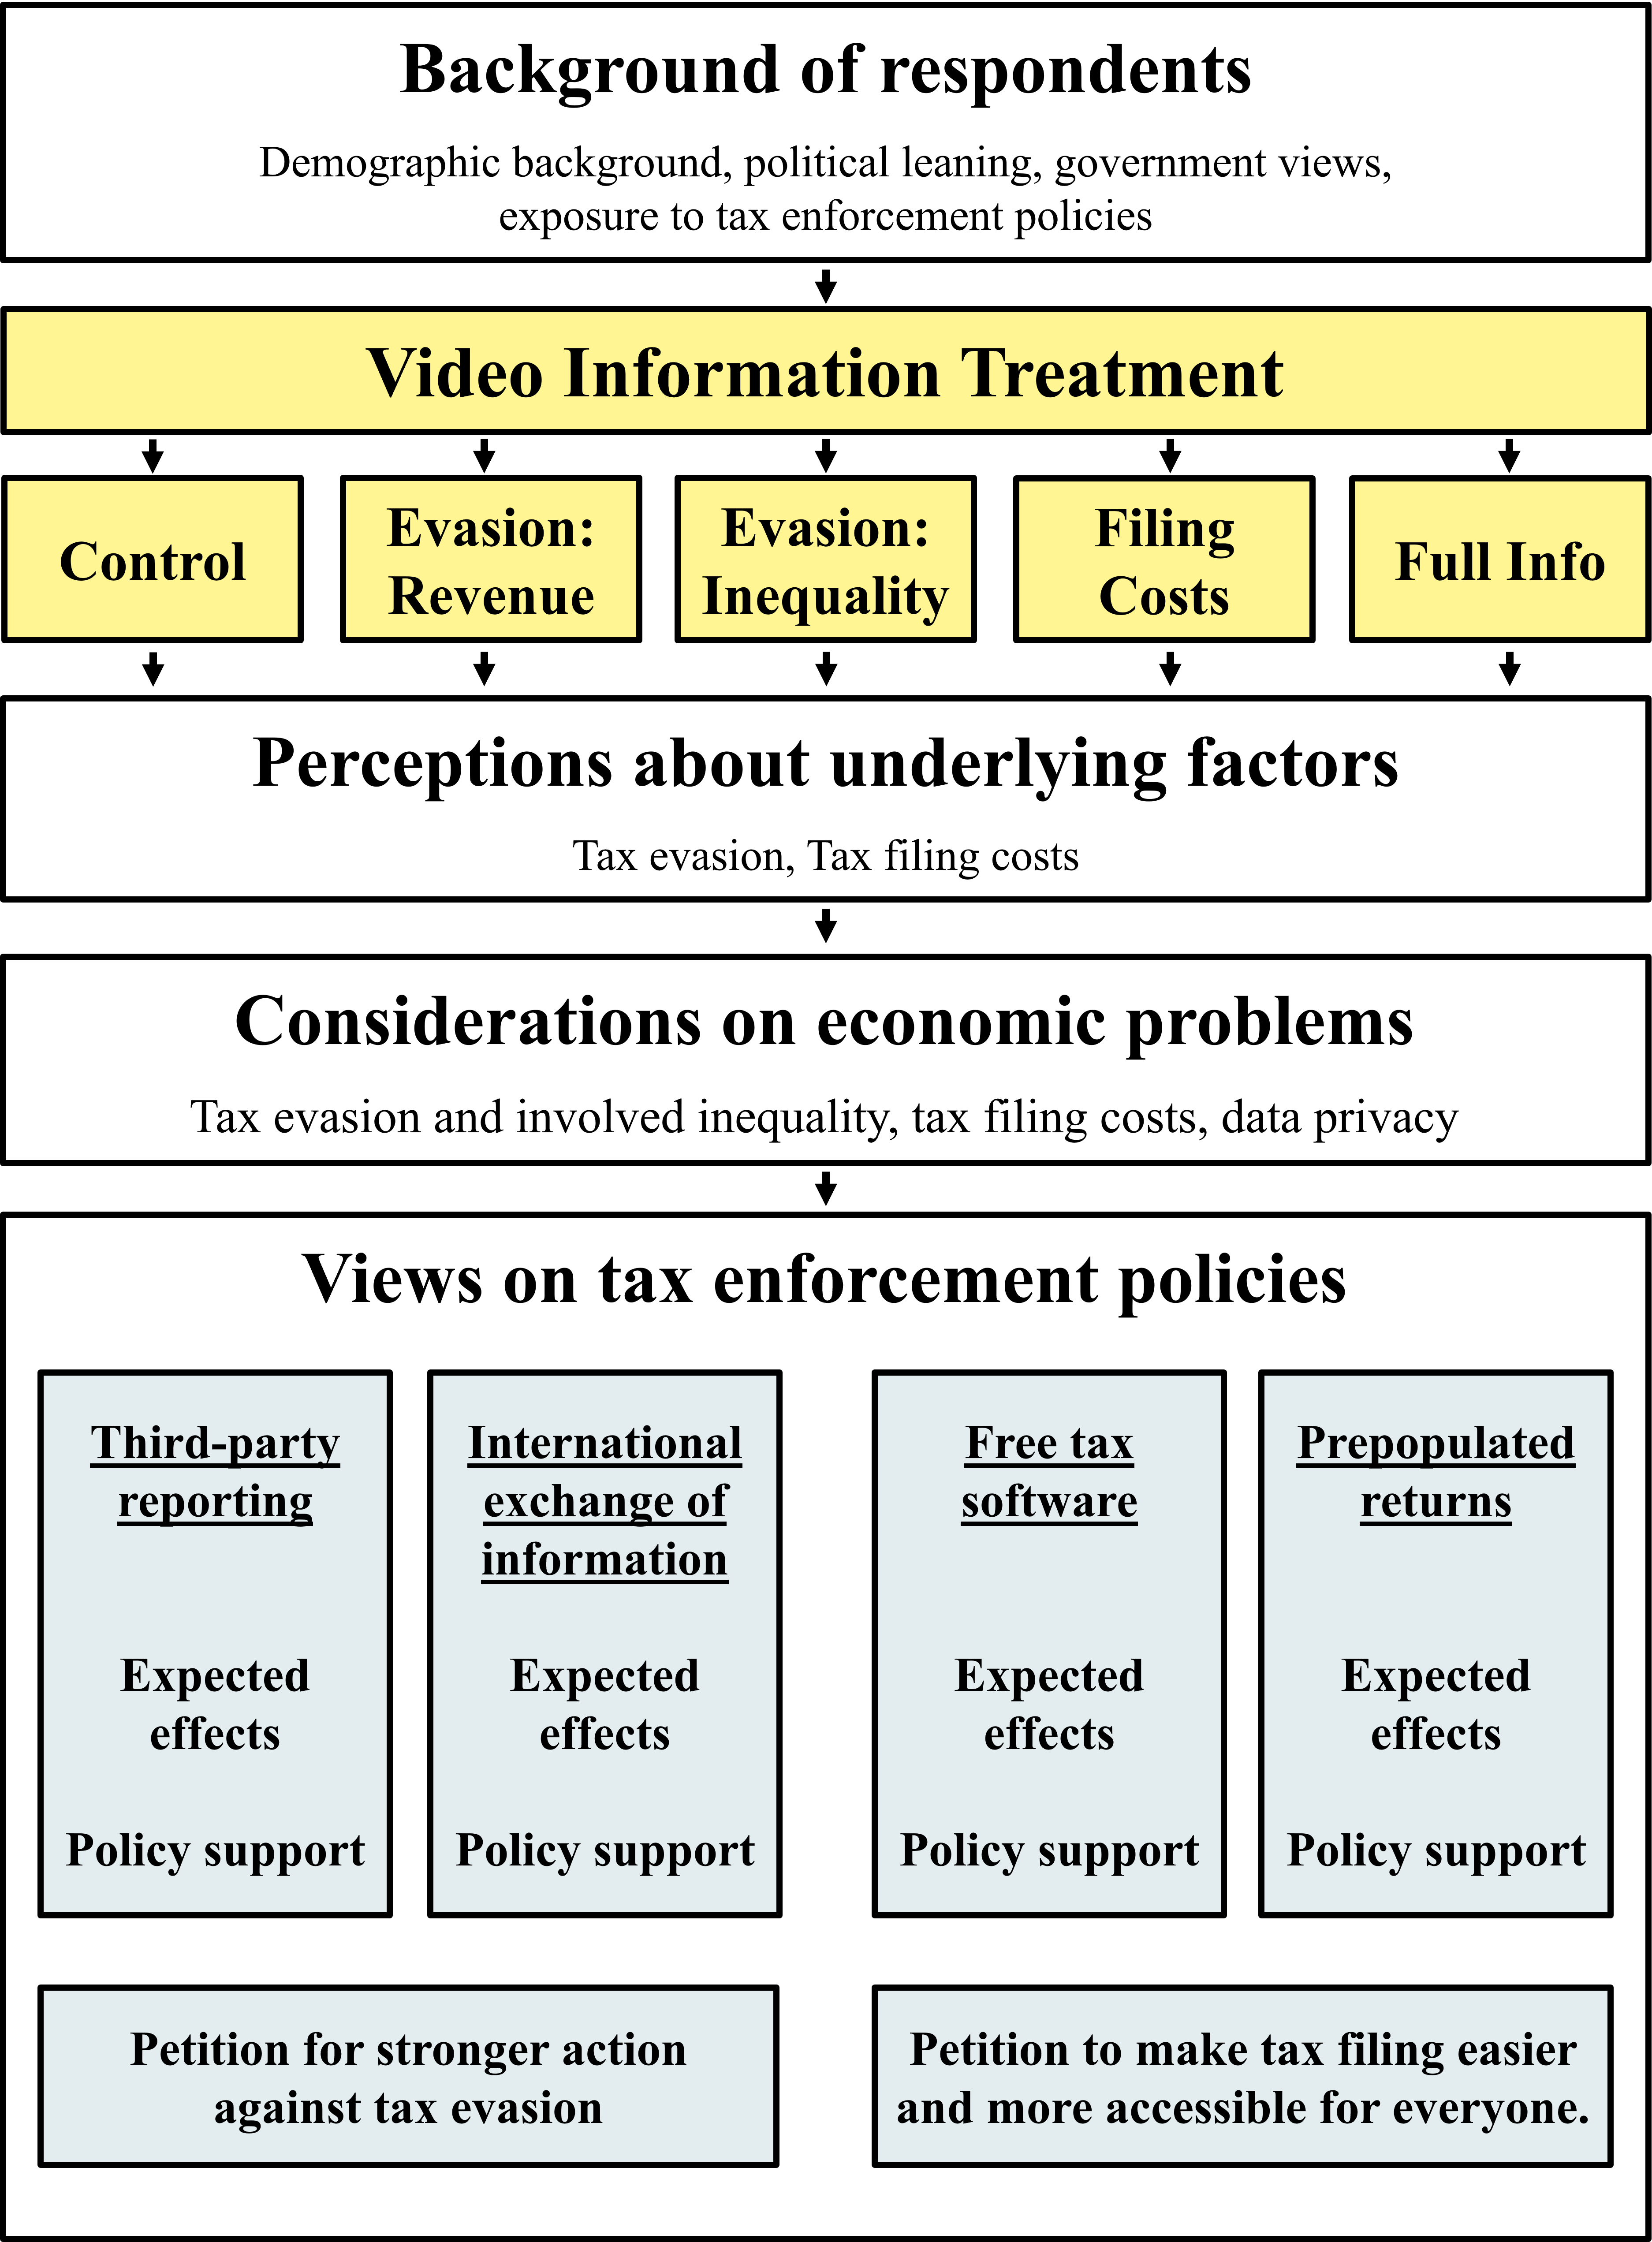
\includegraphics[width=1.05\linewidth]{Figures_Slides/Survey_Overview_Treatments.png}
%  \end{column}
%\end{columns}
%\hfill
%\vfill
%\end{frame}

\begin{frame}[label=Third_Party_Reporting]
  \begin{center}
 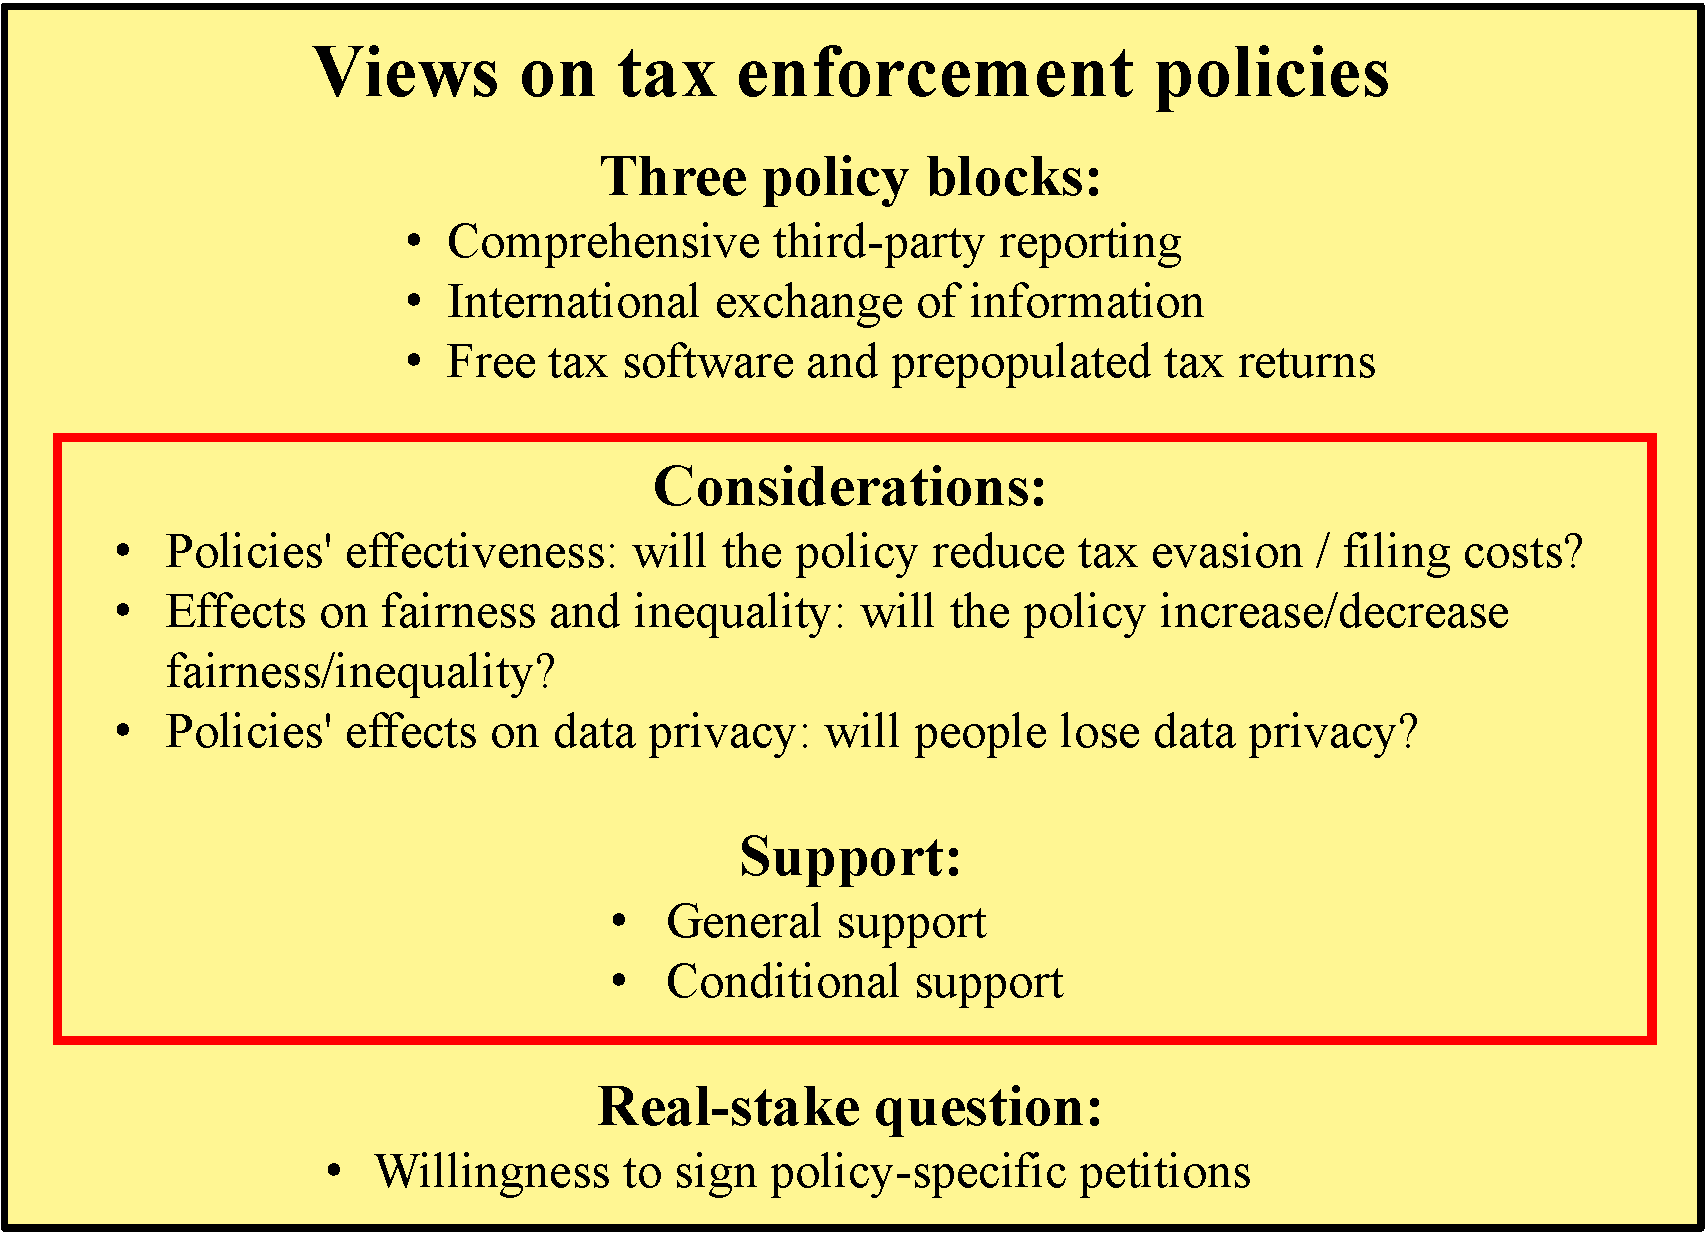
\includegraphics[width=0.65\textwidth]{Figures_Slides/Survey_Overview_Policy_Views_1.pdf} \\
  \end{center}
  %\vspace{0.1cm}
  \begin{center}
 % <-- Breite nach Wunsch anpassen
    The structure of the questionnaire is the same for each policy. \hyperlink{Third_Party_Reporting_Appendix}{\beamergotobutton{A: TPR}}
    \end{center}
    \begin{center}
\begin{minipage}{0.65\textwidth}

    \begin{enumerate}
        \item Short introduction to the policy.
        \item Policy-related considerations/expectations.
        \item Policy support. (general \& conditional)
    \end{enumerate}
  \end{minipage}
  \end{center}
\end{frame}

\begin{frame}[label=Petitions]
  \begin{center}
    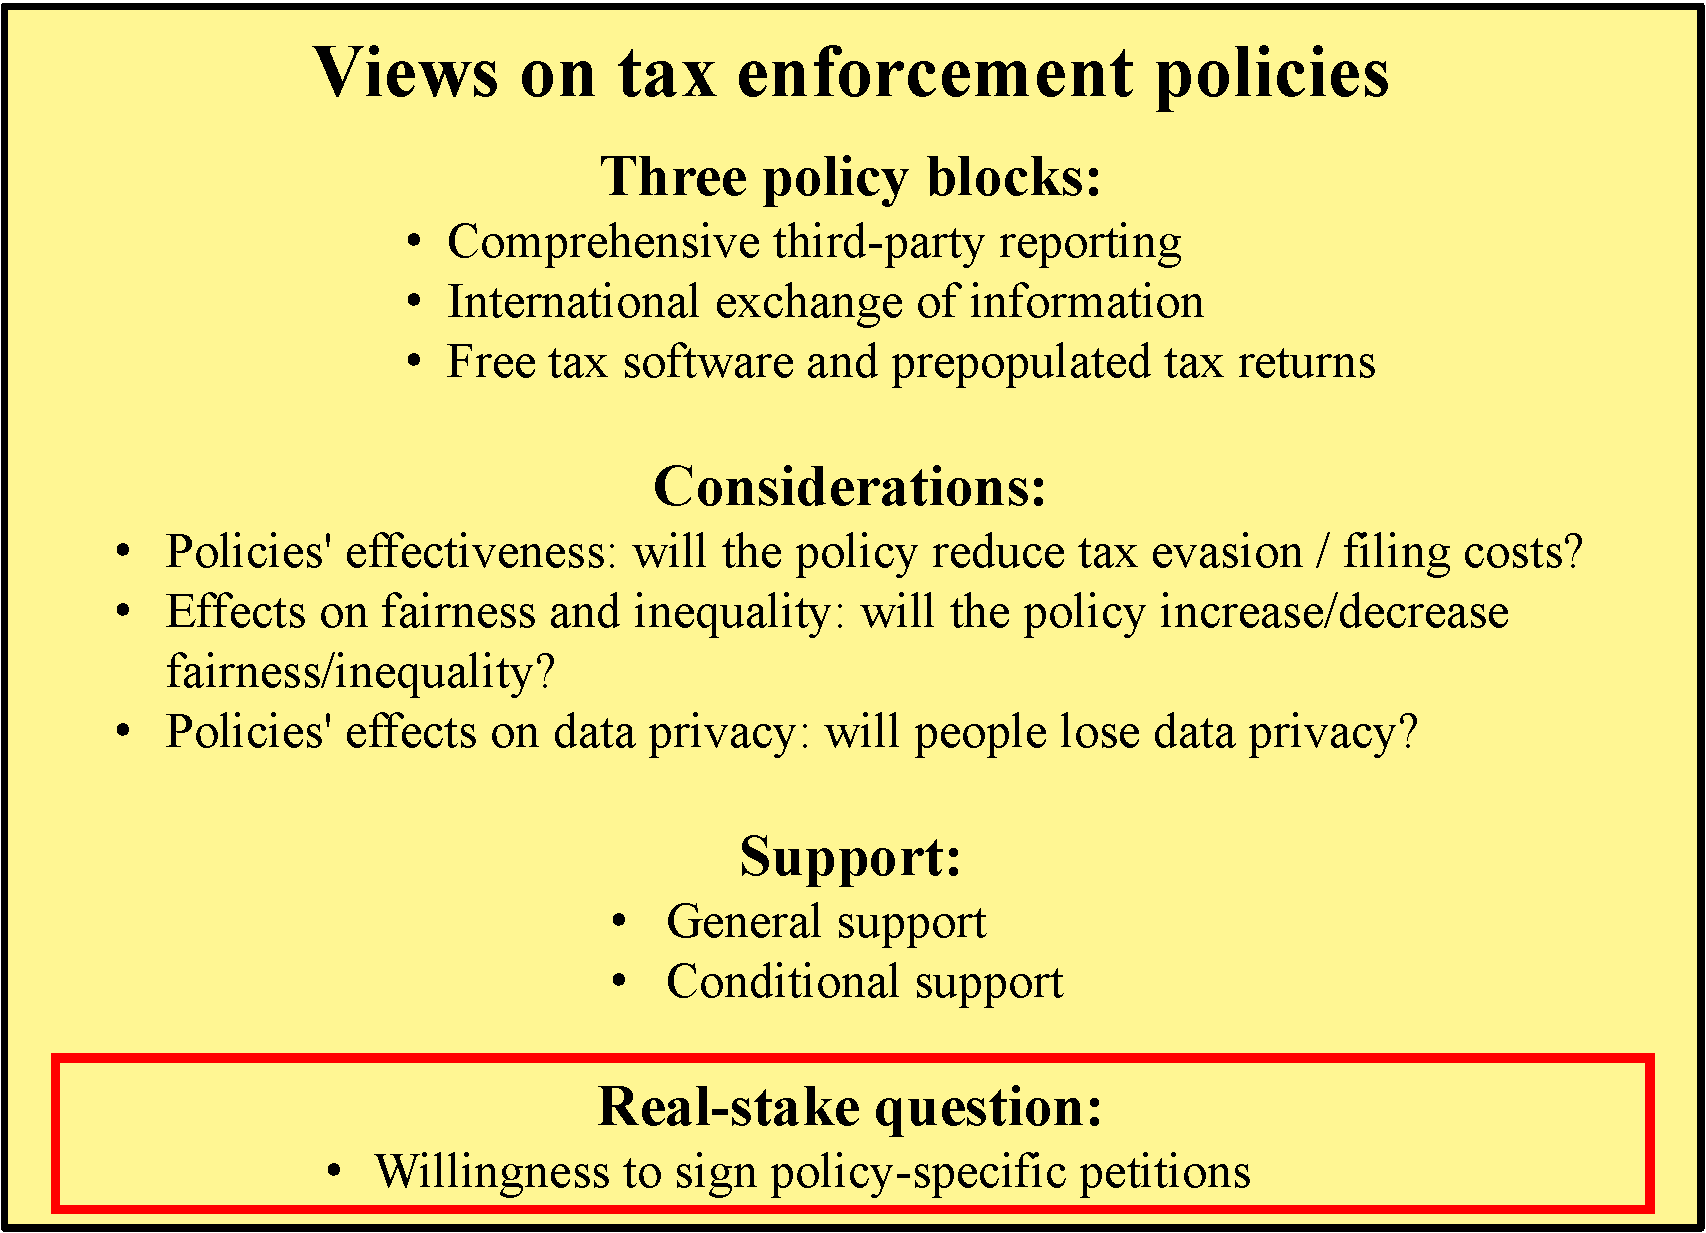
\includegraphics[width=0.65\textwidth]{Figures_Slides/Survey_Overview_Policy_Views_2.pdf} \\
  \end{center}

  

We ask respondents if they want to support \alert{petitions} that aim at policies very similar to our policies from the survey.  \hyperlink{Petitions_Appendix}{\beamergotobutton{A: Petitions}}

  \footnotesize % make the font smaller only for the table
  \begin{tabularx}{\textwidth}{*{2}{>{\centering\arraybackslash}X}}
    \begin{enumerate}
      %\item TPR$^{+}$ $\times$ \\Tax evasion$^{-}$
      \item \alert{in favor} of comprehensive \alert{third- party reporting} to act against tax evasion.
    \end{enumerate} &
    %\begin{enumerate}
    %\setcounter{enumi}{1} % start at 2
    %  %\item TPR$^{-}$ $\times$ \\Data privacy$^{+}$
    %  \item \alert{against} comprehen- sive \alert{third-party reporting} in order to protect privacy.
    %\end{enumerate} &
    \begin{enumerate}
    \setcounter{enumi}{1} % start at 2
      %\item Filing services$^{+}$ $\times$ \\Filing costs$^{-}$
      \item \alert{in favor of making tax filing easier} and more accessible for everyone.
    \end{enumerate} \\
  \end{tabularx}
  \normalsize % reset font size after the table
\end{frame}

\begin{frame}[allowframebreaks]{Detailed Policies}
\label{DetailedPolicies}
\footnotesize
\textbf{Comprehensive Third Party Reporting} \\
\begin{adjustwidth}{0.75em}{0em}Please carefully read the following explanation of third-party reporting and keep it in mind when answering the following questions.\end{adjustwidth} 
\vspace{0.5em}

\begin{adjustwidth}{1.25em}{1.25em}  \textbf{Explanation:}
To fulfill its functions, the tax authority relies on information from third parties such as employers, banks, and government institutions. Under third-party reporting, tax-relevant information is automatically transmitted from domestic firms and institutions to the tax authority. There are ongoing discussions about whether third-party reporting should be substantially expanded to become more comprehensive. Assume that comprehensive third-party reporting would consist of the following changes:
\begin{itemize}
    \item First, the IRS would receive additional information that is currently not reported. In addition to existing reporting requirements, banks would report the total sum of inflows and the total sum of outflows on each bank account over the course of a year. Note that individual transactions would not be reported; only the annual aggregate amounts.
    \item Second, local tax authorities—that is, tax authorities at the county and state level—would transmit previously unreported information on taxes paid at these level to the IRS (such as property taxes and state and local income taxes).
    \item Third, the IRS would ensure that reported data is received more quickly by introducing stricter submission deadlines for third parties that provide information reports.
\end{itemize}
\end{adjustwidth} 
\vspace{2em}
\textbf{International Exchange of Information}\\
\begin{adjustwidth}{0.75em}{0em} Please carefully read the following explanation of international exchange of information and keep it in mind when answering the following questions.\end{adjustwidth}
\vspace{0.5em}
\begin{adjustwidth}{1em}{1em} \textbf{Explanation:} Tax authorities do not only receive information from domestic sources — they can also obtain data about their residents’ foreign bank accounts through international agreements. In the case of the United States, many foreign banks are required to report information on accounts held by U.S.\ taxpayers directly or through their local tax authorities to the U.S.\ government. In some cases, the U.S.\ also agrees to share similar information with those partner countries, but this depends on the specific agreement in place. \\ 
\end{adjustwidth}
\vspace{5em}
\textbf{Tax Software}\\
\begin{adjustwidth}{0.75em}{0em}Please carefully read the following explanation of tax software and keep it in mind when answering the following questions. \end{adjustwidth}
\begin{adjustwidth}{1.25em}{1.25em} \textbf{Explanation:} Tax software is a computer program used for filing tax returns. It usually provides guidance through tax formulas and explains which deductions might apply..
\end{adjustwidth}
\vspace{2em}
\textbf{Prepopulated Tax Returns}
\begin{adjustwidth}{0.75em}{0em}Please carefully read the following explanation of prepopulated tax returns and keep it in mind when answering the following questions. \end{adjustwidth}
\vspace{0.5em}
\begin{adjustwidth}{1.25em}{1.25em} \textbf{Explanation:} Prepopulated tax returns are forms automatically filled in by the tax authority  based on data they already have (for example data on salaries or interest payments). Taxpayers can review the information, make corrections or additions, and then submit the return.
\end{adjustwidth}
\hfill \hyperlink{Update2}{\beamergotobutton{Back: 2) Updates}}
\end{frame}

\begin{frame}{Policy Support for Information Sharing}
\label{Example:PolicySupportGen}
\begin{table}[!htbp]\centering {\fontsize{6pt}{7pt}\selectfont 
\caption{Support for Third-Party Reporting and International Exchange of Information}
\label{tab:supportTPRIEI}
\begin{threeparttable}
\begin{tabular}{l|cc}
\toprule
& (1) & (2) \\
 & Support & Support  \\
 & TPR  & IEI \\
\midrule
Female                     & - & -  \\
Age                        & - & -  \\
College degree             & - & -  \\
Middle income              & - & -  \\
High income                & - & -  \\
Middle wealth              & - & -  \\
High wealth                & - & -  \\
Self-employed              & - & -  \\
Republican                 & - & -  \\[1em]

Evasion: Revenue        & - & - \\
Evasion: Inequality     & - & - \\
Filing costs            & - & - \\
Full info               & - & - \\[0.5em]

Intercept              & - & - \\
\midrule
Observations                        &- &-      \\
$R^2$                               &- &-   \\
Controls                 &   $\mathbf{X}_{i}^{R}$ &  $\mathbf{X}_{i}^{R}$   \\
\bottomrule
\end{tabular}
\begin{tablenotes}[flushleft]
\item \textit{Notes}:   
\end{tablenotes}
\end{threeparttable}
}
\end{table}
\hfill \hyperlink{posttreatment}{\beamergotobutton{Back: Post Treatment}} \hyperlink{equations1}{\beamergotobutton{Back: Equations}}
\end{frame}

\begin{frame}{Policy Support for Tax Filing Services}
\label{Example:PolicySupportGen}
\begin{table}[!htbp]\centering {\fontsize{6pt}{7pt}\selectfont 
\caption{Support for free tax software and prepopulated tax returns}
\label{tab:supporttaxsoftware}
\begin{threeparttable}
\begin{tabular}{l|cc}
\toprule
& (1) & (2) \\
 & Support & Support  \\
 & TS  & PPR \\
\midrule
Female                     & - & -  \\
Age                        & - & -  \\
College degree             & - & -  \\
Middle income              & - & -  \\
High income                & - & -  \\
Middle wealth              & - & -  \\
High wealth                & - & -  \\
Self-employed              & - & -  \\
Republican                 & - & -  \\[1em]

Evasion: Revenue        & - & - \\
Evasion: Inequality     & - & - \\
Filing costs            & - & - \\
Full info               & - & - \\[0.5em]

Intercept              & - & - \\
\midrule
Observations                        &- &-      \\
$R^2$                               &- &-   \\
Controls                 &  $\mathbf{X}_{i}^{R}$ &  $\mathbf{X}_{i}^{R}$    \\
\bottomrule
\end{tabular}
\begin{tablenotes}[flushleft]
\item \textit{Notes}:   
\end{tablenotes}
\end{threeparttable}
}
\end{table}
\hfill \hyperlink{posttreatment}{\beamergotobutton{Back: Post Treatment}} \hyperlink{equations1}{\beamergotobutton{Back: Equations}}
\end{frame}

\begin{frame}{Perception / Knowledge about Economic Problems}
\label{Example:Knowledge}
\begin{table}[!htbp]\centering {\fontsize{6pt}{7pt}\selectfont 
\caption{Knowledge of Economic Problems}
\label{tab:perception}
\begin{threeparttable}
\begin{tabular}{lcccc}
\toprule
 & (1) & (2) & (3)  \\
 & Perception & Perception & Perception\\
 & Tax Gap & Filing Cost (Time) & Filing Cost (Cost)\\
\midrule
Female                     &-& - & - \\
Age                        &-& - & - \\
College degree             &-& - & - \\
Middle income              &-& - & - \\
High income                &-& - & - \\
Middle wealth              &-& - & - \\
High wealth                &-& - & - \\
Self-employed              &-& - & - \\
Republican                 &-& - & - \\[0.5em]
Evasion: Revenue        & - & - & - \\
Evasion: Inequality     & - & - & - \\
Filing costs            & - & - & - \\
Full info               & - & - & - \\[0.5em]
Intercept              &   -& -   & -  \\
\midrule
True Value & - & - & -\\
\midrule
Observations               & - & - & -       \\
$R^2$                      & - & - & -       \\
Controls                   & $\mathbf{X}_{i}^{R}$& $\mathbf{X}_{i}^{R}$& $\mathbf{X}_{i}^{R}$\\
\bottomrule
\end{tabular}
\begin{tablenotes}[flushleft]
\item \textit{Notes}:
\end{tablenotes}
\end{threeparttable}
}
\end{table}
\hfill \hyperlink{posttreatment}{\beamergotobutton{Back: Post Treatment}} \hyperlink{equations1}{\beamergotobutton{Back: Equations}}
\end{frame}

\begin{frame}{Considerations on Economic Problems}
\label{Example:ConsiderationsEconomicProblems}
\begin{table}[!htbp]\centering {\fontsize{5pt}{6pt}\selectfont 
\caption{Considerations on Economic Problems}
\label{tab:considerationseconomicproblems}
\begin{threeparttable}
\begin{tabular}{l||ccc||cc||cc}
\toprule
 & \multicolumn{3}{c||}{Tax Evasion (Revenue \& Inequality)} & \multicolumn{2}{c||}{Filing Costs} & \multicolumn{2}{c}{Data Privacy}\\[0.5em]
  &(1)  &(2) & (3) & (4)  & (5) & (6) & (7) \\[0.25em]
  & Tax Evasion & Tax Evasion & Tax Evasion & Filing Costs & Filing Costs  & Concerned about & Data Privacy \\  
 & Is a Serious &Is Unequally & Is Important & Are & Are Important  & The Government & Is Important  \\
  &  Problem & Distributed & to Reduce & High& to Reduce & Collecting Data & to Protect  \\
\midrule
Female                     &-& - & - &-& - & - &- \\
Age                        &-& - & - &-& - & - &- \\
College degree                     &-& - & - &-& - & - &- \\
Middle income                      &-& - & - &-& - & - &- \\
High income                        &-& - & - &-& - & - &- \\
Middle wealth                      &-& - & - &-& - & - &- \\
High wealth                        &-& - & - &-& - & - &- \\
Self-employed                      &-& - & - &-& - & - &- \\
Republican                         &-& - & - &-& - & - &- \\[0.5em]
Evasion: Revenue        & - & - & - & - & - & - & -  \\
Evasion: Inequality     & - & - & - & - & - & - & -  \\
Filing costs            & - & - & - & - & - & - & -  \\
Full info               & - & - & - & - & - & - & -  \\[0.5em]
Intercept &- &- &- &- &- &- &-\\
\midrule
Observations                        &-    &-    &-    &-    &-    &-    &-  \\
$R^2$                               &-    &-    &-    &-    &-    &-    &-  \\
Controls                 &  $\mathbf{X}_{i}^{R}$  &  $\mathbf{X}_{i}^{R}$&  $\mathbf{X}_{i}^{R}$&  $\mathbf{X}_{i}^{R}$&  $\mathbf{X}_{i}^{R}$&  $\mathbf{X}_{i}^{R}$&  $\mathbf{X}_{i}^{R}$     \\
\bottomrule
\end{tabular}
\begin{tablenotes}[flushleft]
\item \textit{Notes}:   
\end{tablenotes}
\end{threeparttable}
}
\end{table}
\hfill \hyperlink{posttreatment}{\beamergotobutton{Back: Post Treatment}} \hyperlink{equations1}{\beamergotobutton{Back: Equations}}
\end{frame}

\begin{frame}{Considerations on Information Sharing}
\label{Example:ExpectedEffects}
\begin{table}[!htbp]\centering {\fontsize{4.5pt}{5.25pt}\selectfont 
\caption{Considerations on Third-Party Reporting and International Exchange of Information}
\label{tab:policyconsiderationstpr}
\begin{threeparttable}
\begin{tabular}{l||cc|cc|cc|cc|cc||cc||cc}
\toprule
 & \multicolumn{10}{c||}{Tax Evasion (Revenue \& Inequality)} & \multicolumn{2}{c||}{Filing Costs} & \multicolumn{2}{c}{Data Privacy}\\[0.5em]
 & (1) & (2)  & (3) & (4) & (5)& (6)& (7)& (8)& (9)& (10)& (11)& (12)& (13)& (14) \\[0.5em]
 & \multicolumn{2}{c|}{reduces} & \multicolumn{2}{c|}{reduces} & \multicolumn{2}{c|}{increases}& \multicolumn{2}{c|}{increases} & \multicolumn{2}{c||}{reduces}  & \multicolumn{2}{c||}{reduces} & \multicolumn{2}{c}{concerned about} \\
 & \multicolumn{2}{c|}{tax evasion} & \multicolumn{2}{c|}{admin. costs} & \multicolumn{2}{c|}{tax revenue} & \multicolumn{2}{c|}{fairness} & \multicolumn{2}{c||}{inequality}& \multicolumn{2}{c||}{filing costs} & \multicolumn{2}{c}{data privacy}  \\[0.5em]
  & TPR & IEI  & TPR & IEI & TPR & IEI & TPR & IEI & TPR & IEI & TPR & IEI & TPR & IEI \\
\midrule
Female                     &-& - & - &-& - & -& - &-& - & -& - &-& - & - \\
Age                        &-& - & - &-& - & -& - &-& - & -& - &-& - & - \\
College degree             &-& - & - &-& - & -& - &-& - & -& - &-& - & - \\
Middle income              &-& - & - &-& - & -& - &-& - & -& - &-& - & - \\
High income                &-& - & - &-& - & -& - &-& - & -& - &-& - & - \\
Middle wealth              &-& - & - &-& - & -& - &-& - & -& - &-& - & - \\
High wealth                &-& - & - &-& - & -& - &-& - & -& - &-& - & - \\
Self-employed              &-& - & - &-& - & -& - &-& - & -& - &-& - & - \\
Republican                 &-& - & - &-& - & -& - &-& - & -& - &-& - & - \\[1em]

Evasion: Revenue        & - & - & - & - & - & -& - & - & - & -& - & - & - & - \\
Evasion: Inequality     & - & - & - & - & - & -& - & - & - & -& - & - & - & - \\
Filing costs            & - & - & - & - & - & -& - & - & - & -& - & - & - & - \\
Full info               & - & - & - & - & - & -& - & - & - & -& - & - & - & - \\[0.5em]

Intercept &- &- &- &- &- &- &- &- &-&- &- &- &- & -\\
\midrule
Observations                        &-    &-    &-    &-    &-    &- &-    &-    &-    &-&-    &-    &-    &-    \\
$R^2$                               &-    &-    &-    &-    &-    &- &-    &-    &-    &-&-    &-    &-    &-    \\
Controls                 &  $\mathbf{X}_{i}^{R}$&  $\mathbf{X}_{i}^{R}$&  $\mathbf{X}_{i}^{R}$&  $\mathbf{X}_{i}^{R}$ &  $\mathbf{X}_{i}^{R}$&  $\mathbf{X}_{i}^{R}$ &  $\mathbf{X}_{i}^{R}$&  $\mathbf{X}_{i}^{R}$&  $\mathbf{X}_{i}^{R}$&  $\mathbf{X}_{i}^{R}$&  $\mathbf{X}_{i}^{R}$&  $\mathbf{X}_{i}^{R}$&  $\mathbf{X}_{i}^{R}$ &  $\mathbf{X}_{i}^{R}$   \\
\bottomrule
\end{tabular}
\begin{tablenotes}[flushleft]
\item \textit{Notes}:   
\end{tablenotes}
\end{threeparttable} }
\end{table}
\hfill \hyperlink{posttreatment}{\beamergotobutton{Back: Post Treatment}} \hyperlink{equations1}{\beamergotobutton{Back: Equations}}
\end{frame}

\begin{frame}{Considerations on Tax Filing Services}
\label{Example:ExpectedEffects}
\begin{table}[!htbp]\centering {\fontsize{5.5pt}{6.5pt}\selectfont 
\caption{Considerations on Tax Software and Prepopulated Tax Returns}
\label{tab:considerationsts}
\begin{threeparttable}
\begin{tabular}{l|cc|cc|cc}
\toprule
 & \multicolumn{2}{c|}{Revenue} & \multicolumn{2}{c|}{Filing Costs} & \multicolumn{2}{c}{Data Privacy}\\[0.5em]
 & (1) & (2) & (3) & (4) & (5) & (6) \\[0.5em]
 & \multicolumn{2}{c|}{costly for the} & \multicolumn{2}{c|}{reduces} & \multicolumn{2}{c}{data sharing is}\\
 & \multicolumn{2}{c|}{government} & \multicolumn{2}{c|}{filing costs} & \multicolumn{2}{c}{problematic} \\[0.5em]
  & TS & PPR  & TS & PPR & TS & PPR  \\
\midrule
Female                     &-& - & - &-& - & - \\
Age                        &-& - & - &-& - & - \\
College degree             &-& - & - &-& - & - \\
Middle income              &-& - & - &-& - & - \\
High income                &-& - & - &-& - & - \\
Middle wealth              &-& - & - &-& - & - \\
High wealth                &-& - & - &-& - & - \\
Self-employed              &-& - & - &-& - & - \\
Republican                 &-& - & - &-& - & - \\[1em]

Evasion: Revenue        & - & - & - & - & - & - \\
Evasion: Inequality     & - & - & - & - & - & - \\
Filing costs            & - & - & - & - & - & - \\
Full info               & - & - & - & - & - & - \\[0.5em]

Intercept &- &- &- &- &- &- \\
\midrule
Observations                        &-    &-    &-    &-    &-    &- \\
$R^2$                               &-    &-    &-    &-    &-    &- \\
Controls                            & $\mathbf{X}_{i}^{R}$    & $\mathbf{X}_{i}^{R}$    & $\mathbf{X}_{i}^{R}$    & $\mathbf{X}_{i}^{R}$     & $\mathbf{X}_{i}^{R}$    & $\mathbf{X}_{i}^{R}$  \\
\bottomrule
\end{tabular}
\begin{tablenotes}[flushleft]
\item \textit{Notes}:   
\end{tablenotes}
\end{threeparttable} }
\end{table}
\hfill \hyperlink{posttreatment}{\beamergotobutton{Back: Post Treatment}} \hyperlink{equations1}{\beamergotobutton{Back: Equations}}
\end{frame}


\begin{frame}{Conditional Suppport for Third-Party Reporting}
\label{Example:PolicySupportCond}
\begin{table}[!htbp]\centering {\fontsize{5pt}{6pt}\selectfont 
\caption{Conditional Support for Third-Party Reporting}
\label{tab:conditionalsupporttpr}
\begin{threeparttable}
\begin{tabular}{l|c}
\toprule
 & (1)\\
 & Support \\
 \midrule
Support for comprehensive third-party reporting if \\[0.25em]
--it applied equally to all taxpayers. &-\\[0.25em]
--it applied primarily to businesses.&-\\[0.25em]
--it focuses on high-income individuals. &- \\[0.25em]
--it focuses on large enterprises.&- \\[0.25em]
--the data collected could only be used for purposes  & - \\
related to tax enforcement and tax administration.\\[0.25em]
--the data collected would also be used to offer & - \\
prepopulated tax returns & - \\[0.25em]
--the data collected could only be used to offer & - \\
prepopulated tax returns & - \\[0.25em]
--taxpayers could voluntarily choose to have their own & -\\ 
data covered.\\[1em]
Evasion: Revenue        & - \\
Evasion: Inequality     & - \\
Filing costs            & - \\
Full info               & - \\[0.5em]
Intercept &-  \\
\midrule
Observations                        &-       \\
$R^2$                               &-    \\
Controls                 &    $\mathbf{X}_{i}^{R}$      \\
\bottomrule
\end{tabular}
\begin{tablenotes}[flushleft]
\item \textit{Notes}: Note that the later 3 conditions are asked later in the survey, namely after respondents are informed about the existence of prepopulated tax returns.   
\end{tablenotes}
\end{threeparttable}}
\end{table} 
\hfill \hyperlink{posttreatment}{\beamergotobutton{Back: Post Treatment}} \hyperlink{equations2}{\beamergotobutton{Back: Equations}}
\end{frame}

\begin{frame}{Detailed Data Privacy Concerns}
\label{Example:DetailedDataPrivacy}
\begin{table}[!htbp]\centering {\fontsize{5pt}{6pt}\selectfont 
\caption{Detailed Data Privacy Concerns}
\label{tab:detaileddataprivacy}
\begin{threeparttable}
\begin{tabular}{l|c}
\toprule
& (1) \\
 & concerned about \\
 & data privacy \\
 \midrule
\textit{Conditions} \\[0.25em]
if third-party reporting includes.. & \\[0.25em]
-employment data in general & - \\[0.25em]
-employment data limited to tax relevant information & - \\[0.25em]
-general health insurance data & - \\[0.25em]
-health insurance data limited to tax-relevant financial information & -\\[0.25em]
-general bank account data & - \\[0.25em]
-bank account data limited to tax-relevant information & - \\[0.25em]
-payment data & - \\[0.25em]
-payment data limited to tax-relevant information & - \\[1em]
\textit{Treatments} \\[0.25em]
Evasion: Revenue        & - \\[0.25em]
Evasion: Inequality     & - \\[0.25em]
Filing costs            & - \\[0.25em]
Full info               & - \\[1em]
Intercept &-  \\
\midrule
Observations                        &-       \\
$R^2$                               &-    \\
Controls                 & $\mathbf{X}_{i}^{R}$      \\
\bottomrule
\end{tabular}
\begin{tablenotes}[flushleft]
\item \textit{Notes}:   
\end{tablenotes}
\end{threeparttable}}
\end{table} 
\hfill \hyperlink{posttreatment}{\beamergotobutton{Back: Post Treatment}} \hyperlink{equations2}{\beamergotobutton{Back: Equations}}
\end{frame}

\begin{frame}{Private or Government Provider}
\label{Example:DetailedDataPrivacy}
\begin{table}[!htbp]\centering {\fontsize{6pt}{7pt}\selectfont 
\caption{Private or Government Tax Software Provider}
\label{tab:taxsoftwareprovider}
\begin{threeparttable}
\begin{tabular}{l|c}
\toprule
& (1) \\
 & Tax Authority Should \\
 & Provide Tax Software \\
 \midrule
\textit{Considerations} \\[0.25em]
-In general & \\[0.25em]
-In terms of reducing time and monetary costs for taxpayers & - \\[0.25em]
-In terms of overall costs to the society & - \\[0.25em]
-In terms of data privacy & - \\[1em]
\textit{Treatments} \\[0.25em]
Evasion: Revenue        & - \\[0.25em]
Evasion: Inequality     & - \\[0.25em]
Filing costs            & - \\[0.25em]
Full info               & - \\

\midrule
Observations                        &-       \\
$R^2$                               &-    \\
Controls                 & $\mathbf{X}_{i}^{R}$      \\
\bottomrule
\end{tabular}
\begin{tablenotes}[flushleft]
\item \textit{Notes}:   
\end{tablenotes}
\end{threeparttable}
}
\end{table} 
\hfill \hyperlink{posttreatment}{\beamergotobutton{Back: Post Treatment}} \hyperlink{equations2}{\beamergotobutton{Back: Equations}}
\end{frame}


\begin{frame}{Drivers of Policy Support}
\label{Example:PolicySupportDrivers}
\vspace{-0.5em}
\begin{table}[!htbp]\centering {\fontsize{6pt}{7pt}\selectfont 
\caption{Drivers of policy support}
\label{tab:PolicySupportDrivers}
\begin{threeparttable}
\begin{tabular}{l|cccc}
\toprule
& (1) & (2) & (3) & (4) \\
 & Support & Support & Support & Support  \\
 & TPR  & IEI & TS & PPR \\
\midrule
\textit{Controls} \\
Republican                 & - & - & - & - \\
... \\[1em]

\textit{Considerations on economic problems}\\
--Tax evasion is a serious problem        & - & -& - & - \\
--Tax evasion is unequally distributed     & - & -& - & - \\
--Tax evasion is important to reduce & - & -& - & - \\
--Filing costs are high               & - & -& - & - \\
--Filing costs are important to reduce    & - & -& - & - \\
--Concerned about the government collecting data    & - & -& - & - \\
--Data privacy is important to protect    & - & -& - & - \\[1em]

\textit{Considerations on policies regarding...}\\
--Tax evasion and revenue    & - & -& - & - \\
--Inequality          & - & -&   &   \\
--Filing costs        & - & -& - & - \\
--Data privacy        & - & -& - & - \\[1em]

Intercept              & - & - & - & -\\
\midrule
Observations                        &- &- & - & -     \\
$R^2$                               &- &- & - & -  \\
Controls                 & $\mathbf{X}_{i}^{R}$  & $\mathbf{X}_{i}^{R}$ & $\mathbf{X}_{i}^{R}$  & $\mathbf{X}_{i}^{R}$    \\
\bottomrule
\end{tabular}
%\begin{tablenotes}[flushleft]
%\item \textit{Notes}:   
%\end{tablenotes}
\end{threeparttable}
}
\end{table} 
\hfill \hyperlink{equations3}{\beamergotobutton{Back: Equations}}
\end{frame}

\begin{frame}{3) Survey \& Estimation: Equations (4)} 
\label{equations4}
To analyze how pre treatment outcome variables are distributed among demographic groups, we run regressions according to Equations \ref{eq:governmenttrust}-\ref{eq:inequalityseriousproblem}.\footnote[9]{Note that now, we do not include $\mathbf{T}_i$ and we do only use $\mathbf{X}_i^{D}.$} 
\begin{align}
    \label{eq:governmenttrust}
    \text{$Government\_Trust_i$} 
        &= \alpha + \boldsymbol{\beta}^{\top}\mathbf{X}_i^{D} + \varepsilon_i
         \\
   \text{$Government\_More\_Involved_i$} 
        &= \alpha + \boldsymbol{\beta}^{\top}\mathbf{X}_i^{D} + \varepsilon_i \\
   \text{$Government\_Quality_i$} 
        &= \alpha + \boldsymbol{\beta}^{\top}\mathbf{X}_i^{D} + \varepsilon_i \\
    \label{eq:inequalityseriousproblem}
    \text{$Inequality\_Serious\_Problem_i$} 
        &= \alpha + \boldsymbol{\beta}^{\top}\mathbf{X}_i^{D} + \varepsilon_i 
\end{align}
\hfill \hyperlink{GovernmentViews}{\beamergotobutton{Figures}} 
\end{frame}

\begin{frame}{Government Views and Views on Inequality}
\label{GovernmentViews}
\begin{table}[!htbp]\centering {\fontsize{7pt}{8pt}\selectfont 
\caption{Government Views and Views on Inequality}
\label{tab:government_inequality_views}
\begin{threeparttable}
\begin{tabular}{lcccc}
\toprule
 & (1) & (2) & (3) & (4)  \\
 & Trust in & Government Should & Quality of & Inequality is \\
 & Government & Be More Involved & Government Services & a serious problem\\
\midrule
Female                     &-& - & -& - \\
Age                        &-& - & -& - \\
College degree             &-& - & -& - \\
Middle income              &-& - & -& - \\
High income                &-& - & -& - \\
Middle wealth              &-& - & -& - \\
High wealth                &-& - & -& - \\
Self-employed              &-& - & -& - \\
Republican                 &-& - & -& - \\[0.5em]
Intercept              &   -& -   & -& -  \\
\midrule
Observations               &-        &-        &-& -       \\
$R^2$                      &-        &-        &-& -       \\
Controls                   &$\mathbf{X}_i^{D}$&$\mathbf{X}_i^{D}$&$\mathbf{X}_i^{D}$&$\mathbf{X}_i^{D}$\\
\bottomrule
\end{tabular}
\begin{tablenotes}[flushleft]
%\footnotesize
\item \textit{Notes}: 
\end{tablenotes}
\end{threeparttable}
}
\end{table} 

\hfill \hyperlink{equations4}{\beamergotobutton{Back: Equations}}
\end{frame}

\begin{frame}{Exposure to Tax Filing and Evasion}
\label{Example:PolicySupportDrivers}
\begin{table}[!htbp]\centering {\fontsize{7pt}{8pt}\selectfont 
\caption{Exposure to Tax Filing and Evasion}
\label{tab:exposure}
\begin{threeparttable}
\begin{tabular}{lcccc}
\toprule
 & (1) & (2) & (3) & (4) \\
 & Exposure: & Exposure: & Exposure: & Exposure: \\
 & Tax Filing & Tax Software & Filing Mistakes & Evasion \\
\midrule
Female                     &-& - & - &-  \\
Age                        &-& - & - &-  \\
College degree             &-& - & - &-  \\
Middle income              &-& - & - &-  \\
High income                &-& - & - &-  \\
Middle wealth              &-& - & - &-  \\
High wealth                &-& - & - &-  \\
Self-employed              &-& - & - &-  \\
Republican                 &-& - & - &-  \\[0.5em]
Intercept              &   -& -   & -  &   -\\
\midrule
Observations               &        &        &        &        \\
$R^2$                      &        &        &        &        \\
Controls                   &$\mathbf{X}_{i}^D$&$\mathbf{X}_{i}^D$&$\mathbf{X}_{i}^D$&$\mathbf{X}_{i}^D$\\
\bottomrule
\end{tabular}
\begin{tablenotes}[flushleft]
\item \textit{Notes:}
\end{tablenotes}
\end{threeparttable}
}
\end{table} 

\hfill \hyperlink{equations4}{\beamergotobutton{Back: Equations}}
\end{frame}

\begin{frame}{Variables: Control Variables}
\label{Controlvariables}
{\tiny
\[
\begin{array}{ccc}
X_i^{D} =
\left(
\begin{array}{c}
\textit{Gender} \\[0.2em]
\textit{Race} \\[0.2em]
\textit{Region} \\[0.2em]
\textit{Urban/Rural} \\[0.2em]
\textit{Age} \\[0.2em]
\textit{Marital status} \\[0.2em]
\textit{Education} \\[0.2em]
\textit{Household characteristics} \\[0.2em]
\textit{Homeowner/tenant} \\[0.2em]
\textit{Employment status}\\[0.2em]
\textit{Student} \\[0.2em]
\textit{Household income} \\[0.2em]
\textit{Household wealth} \\[0.2em]
\textit{Income source} \\[0.2em]
\textit{Political affiliation}
\end{array}
\right)

& \qquad\qquad &
X_i^{R} =
\left(
\begin{array}{c}
\textit{Gender} \\[0.2em]
\textit{Race} \\[0.2em]
\textit{Region} \\[0.2em]
\textit{Urban/Rural} \\[0.2em]
\textit{Age} \\[0.2em]
\textit{Marital status} \\[0.2em]
\textit{Education} \\[0.2em]
\textit{Household characteristics} \\[0.2em]
\textit{Homeowner/tenant} \\[0.2em]
\textit{Employment status}\\[0.2em]
\textit{Student} \\[0.2em]
\textit{Household income} \\[0.2em]
\textit{Household wealth} \\[0.2em]
\textit{Income source} \\[0.2em]
\textit{Political affiliation} \\[0.2em]
\textit{Government trust} \\[0.2em]
\textit{Government more involved} \\[0.2em]
\textit{Government quality of services} \\[0.2em]
\textit{Inequality is a serious problem}\\[0.2em]
\textit{Exposure to tax filing}\\[0.2em]
\textit{Exposure to tax software}\\[0.2em]
\textit{Exposure to filing mistakes}\\[0.2em]
\textit{Exposure to tax evasion}
\end{array}
\right)

\end{array}
\]
}
\hfill \hyperlink{pretreatment}{\beamergotobutton{Back to Pre Treatment}} \hyperlink{equations1}{\beamergotobutton{Back to Equations}}
\footnotetext[10]{\tiny Note that for the demographics we include more disggregated variables. E.g. for Race we include $Black_i$, $Hispanic_i$, $Asian_i$, $Other\_Race_i$}
\end{frame}
\begin{frame}[allowframebreaks]
  \frametitle{Literature}
  \printbibliography
\end{frame}



%----------------------------------------------------------------------------------------
\end{document} 